\section{Einleitung}
\subsection{Motivation}
Entsprechend der \textit{Programmstruktur der EU-Fonds EFRE, ESF, ELER und EMFF in Sachsen-An"-halt für die Förderperiode 2014 bis 2020}\footnote{\url{http://www.europa.sachsen-anhalt.de/fileadmin/Bibliothek/Politik_und_Verwaltung/StK/Europa/Dokumente/Programmstruktur_EU-Fonds.pdf}} besteht ein Schwerpunkt in der 
\textit{Förderung der Anpassung an den Klimawandel sowie der Risikoprävention und des Risikomanagements}. Danach soll \say{$\dots$ die Möglichkeit eröffnet werden, dringende Maßnahmen der Kommunen mit investivem Charakter zur Verbesserung des kommunalen Hochwasserschutzniveaus zu fördern. Darüber hinaus sollen Vorhaben unterstützt werden, die die Beseitigung oder Minderung von sowie Vorbeugung gegen Vernässung oder Erosion zum Ziel haben.}\

Für die Umsetzung der Förderziele sind großmaßstäbige und flächendeckende Grundlagendaten insbesondere zu grund- und hochwasserbeeinflussten Böden notwendig, die eine wichtige Regulierungsfunktion für den Flächenwasserhaushalt besitzen. So fungieren grund- und hochwasserbeeinflussten Böden beispielsweise als Retentionskörper von Niederschlagswasser oder als Orte des Rückhalts und der Freisetzung von Schadstoffen. Darüber hinaus haben Böden eine dämpfende oder verstärkende Wirkung bei Klimaänderungen (Vernässung oder Austrocknung, Überschwemmung).\

Für die Fläche des Landes Sachsen-Anhalt stehen mittel- bis kleinmaßstäbige, bodenkundliche Übersichtkarten im Maßstab 1:400\,000 und 1:200\,000 zur Vefügung. Den Maßstabsbereich 1:50\,000 deckt die (digitale) Vorläufige Bodenkarte 1:50\,000 von Sachsen-Anhalt (VBK\,50) ab \citep{Hartmann2005,Hartmann2006,Hartmann2014}.

Im großmaßstäbigen Maßstabsbereich existiert noch keine konsistente Bodenkarte. Neben der Bodenschätzung und Forstlichen Standortskartierung, die die landwirtschaftlichen Nutzfläche bzw. Wälder abdecken und in Sachsen-Anhalt in digitaler Form vorliegen \citep{Gutteck1999,Hartmann2006},  sind weitere Kartierungen aus DDR-Zeiten (Projekt- und Moorkartierungen u.a.) vorhanden. Die Kartenwerke sind durch unterschiedliche Nomenklaturen sowie geometrische Zielmaß"-stä"-be gekennzeichnet \citep{Moeller-etal2012catena,Hartmann2014}, basieren aber alle auf der Bodenform. Abbildung \ref{fig:soildata} veranschaulicht Unterschiede bodenkundlich relevanter Kartenwerke hinsichtlich Maßstab, geometrischer Auf"-lö"-sung und räumlicher Differenzierung (vgl. Tab. \ref{tab:daten}, S. \pageref{tab:daten}). 

\begin{figure}[t]
\centering\includegraphics[height=0.45\textheight]{figures/bode_data}
\caption[Überlagerung bodenkundlich relevanter Kartenwerke am Beispiel des Testgebietes \textit{Bode}.]{Überlagerung bodenkundlich relevanter Kartenwerke am Beispiel des Testgebietes \textit{Bode} (vgl. Abb. \ref{fig:ug}). MMK -- Mittelmaßstäbige Standortskartierung $|$ VBK\,50 -- Vorläufige Bodenkarte 1:50\,000 $|$ MMK -- Mittelmaßstäbige Landwirtschaftliche Standortkartierung $|$ BS -- Bodenschätzung $|$ GK\,25 -- Geologische Karte 1:25\,000 $|$ FSK -- Forstliche Standortskartierung.}\label{fig:soildata}
\end{figure}


\begin{table}[t]
  \centering
  \caption[Bodenkundliche Eingangsdaten im Testgebiet \textit{Bode}.]{Bodenkundliche Eingangsdaten im Testgebiet \textit{Bode}.}\label{tab:daten}
	\vspace*{6pt}
  \begin{threeparttable}
    \begin{tabularx}{\textwidth}{l|m{1.4cm}|m{1.55cm}|X|X|X|X|X|X}
    \toprule
    \multirow{2}[0]{*}{\textbf{Quellen}\tnote{1}} & \multirow{2}[0]{*}{\textbf{Maßstab}} & \multirow{2}[0]{*}{\textbf{Wichtung}} &\multirow{2}[0]{*}{\textbf{Tiefe}\tnote{2}} & \multicolumn{5}{c}{\textbf{Zielmerkmale}\tnote{3}}\\
				  &			      & 		  &		         & FB 	        & GEN	     & SKE	    & C	  & BST \\\midrule
    MMK			& 1:100\,000& 0,2   & 12         & $(\times)$   &		       &$(\times)$  & $((\times))$ &$(\times)$\\\midrule
    VBK\,50			& 1:50\,000	& 0,5   & 12         & $(\times)$   &$\times$  &$\times$  & $\times$ &  $(\times)$\\\midrule
    GK\,25			& 1:25\,000	& 0,8   & 20& $((\times))$ &$\times$  &$((\times))$  & $((\times))$   &  \\\midrule
    BS				& 1:10\,000	& 1     & 10         & $(\times)$   &$(\times)$&$\times$& $\times$   &  $(\times)$\\\midrule
    FSK\,10			& 1:10\,000	& 1     & 20         & $\times$     &$\times$  &$\times$  & $\times$   &  $\times$\\\bottomrule
    \end{tabularx}%
    \begin{tablenotes}
		\item[1] \begin{asparaitem}
		\item MMK -- Mittelmaßstäbige Standortkarte der landwirtschaftlichen Nutzfläche
		\item VBK\,50 -- Vorläufige digitale Bodenkarte von Sachsen-Anhalt
		\item GK\,25 -- Geologische Karte mit Übersetzung der lithologischen Angaben in Substrate entsprechend \citet{KA5}		\item BS -- Unterlagen der Bodenschätzung Karte der Klassenflächen (Folie42)/Grablochbeschriebe
		\item FSK\,10 -- Forstliche Standortskarte mit übersetzten Forstbodenformen entsprechend \citet{KA5}
		\end{asparaitem}
    		\item[2] Tiefe, bis zu der die Auswertung der entsprechenden Karten für ProBoSa erfolgt. Die GK\,25 enthält zum Teil keine Angaben im oberen Bereich.
		\item[3] \begin{inparaitem}
		\item FB -- Feinboden 
		\item GEN -- Genese/Geogenese 
		\item C -- Carbonat 
		\item BST -- Bodensubtyp
		\item SKE -- Grobboden
		\end{inparaitem}\newline
		Die Aussagemöglichkeiten bedeuten:
		\begin{asparaitem}
		\item	$\times$ -- verwendbare Angaben vorhanden
		\item $(\times)$ -- Angaben vorhanden, Einschränkungen durch den Maßstab, die Aggregierung oder unscharfe Daten
    \item $((\times))$ -- Angaben nicht oder nicht durchgängig vorhanden, Ableitung durch Sekundärwissen möglich.
		\end{asparaitem}
  \end{tablenotes}
 \end{threeparttable}   
\end{table}%


%\subsection{Bisherige Ansätze zur Auswertung der Bodenschätzung}
%\citet{Wallbaum1991} wertete Analyseergebnisse zu 4000 Bodenschichten von Grablochbeschrieben auf dem Gebiet der neuen Bundesländer statistisch aus und konnte darauf basierend für einige wichtige Bodenparameter Übersetzungsschlüssel für den Transfer in die TGL\,24300- und KA\,3-Nomenklatur erstellen. Zu den Thesen dieser Arbeit gehörte u.a., dass die Qualität der Bodenschätzungsunterlagen unterschiedlich ist und die Interpretation der Bodenschätzung gemarkungs- bzw. bodenschätzerspezifisch erfolgen sollte. Wallbaum stellt heraus, dass bei der pedologischen Charakterisierung der Klassenflächen der regionale Kontext einbezogen werden muss. Eine Charakterisierung einer Klassenfläche als (homogenes) Pedotop allein auf Grundlage des bestimmenden Grabloches, würde der Heterogenität der Bodendecke nicht gerecht. Aussagen zu Bodenarten bzw. Substrattypen waren besser ableitbar als Aussagen zu Horizontbezeichnungen, Bodentypen und Bodentypenspektren von Flächeneinheiten.\
%
%In Niedersachsen wird bereits seit Ende der 70er Jahre an der dv-gestützten Übersetzung der Bodenschätzung gearbeitet und der Übersetzungsschlüssel laufend dem neuen Erkenntnisstand angepasst. Der Schlüssel integriert neben den Bodenschätzungsdaten selber auch geomorphographische  und Klimadaten. Es wurden auch regionale und andere Differenzierungen des Standardregelwerkes implementiert \citep{NBIS2003}.


\subsection{Bisherige Arbeiten zur digitalen Bodenkartierung in Sachsen-Anhalt}\label{sec:dsm}
In Sachsen-Anhalt sind eine Reihe von Arbeiten, die sich mit der Erstellung neuer Bodenkarten auf Grundlage vorhandener Bodendaten und Nutzung bodenrelevanter Datenbestände beschäftigen, durchgeführt worden. Sie können hinsichtlich der verwendeten Methoden in (1.) expertenbasierte Regelwerke und (2.) Verfahren des maschinellen Lernens unterschieden werden.

\begin{enumerate}
\item \citet{BehrensScholten2003a} erstellten für das Schwarzerdegebiet in Sachsen-Anhalt eine bodentypologische Rasterkarte für den Maßstabsbereich 1:25\,000 bis 1:50\,000. Grundlage war eine Faktorenanalyse von Klimarasterdaten, Reliefattributen eines digitalen Höhenmodells sowie des Karbonatgehaltes der Mittelmaßstäbigen Landwirtschaftlichen Standortskartierung. Die Ausweisung von Auesedimenten erfolgt anhand einer Überflutungssimulation. Es wurde ein teilweise statistisch begründetes, teilweise expertenbasiertes Regelwerk aus den Faktoren Klima und Relief sowie Löss- und Auenverbreitung aufgestellt, die das Auftreten von Schwarzerden, Kalk-Schwarzerden, Rendzinen, Parabraunerden, Gleyen, Kolluvien und Pseudogleyen bestimmen.\

Die synthetische Konzeptbodenkarte Ostharz  besteht aus den zwei Komponenten \textit{Vorhersage periglaziärer Lagen} und \textit{Reliefanalyse} \citep{ScholtenBehrensHenningsen2001}. Die Reliefanalyse zielt auf die Ausweisung von Gebieten mit Akkumulations- und Abtragungsneigung sowie Arealen mit nur geringer Tendenz zu solifluidalen Verlagerung. Auen und Niederungen wurden auf Grundlage einer hybriden Überflutungssimulation generiert. Die Vorhersage periglaziärer Lagen und ihrer Mächtigkeit basierte auf einer Reihe von Reliefparametern und Informationen zum Ausgangsgestein (Digitale Geologische Karte 1:25\,000). Zur Ausgrenzung quasihomogener Bodenbereiche wurden die flächendeckend ermittelten Mächtigkeiten der periglaziären Lagen und die Ergebnisse der Reliefanalyse klassifiziert und verschnitten. Die Klas"-si"-fi"-zie"-rung erfolgte auf Grundlage von Expertenwissen und unter Einbeziehung der Bodenübersichtskarte 1:200\,000 sowie der bodentypologischen Angaben von Bodenprofilaufnahmen im Ostharzgebiet. Wie schon bei der bodentypologischen Konzeptkarte des Schwarzerdegebietes resultieren die Grenzen der abgeleiteten Bodenbildungsbereiche im Ostharz nicht aus vorhandenen Bodenkarten, sondern aus den nicht bodenkundlichen Eingangsdaten, insbesondere den verwendeten digitalen Geländemodellen.\

\citet{geoflux_MoellerKoschitzki2007lagb} erarbeiteten ein Regelwerk zur reliefbezogenen Plau"-si"-bi"-li"-täts"-über"-prüfung der Vorläufigen Bodenkundlichen Karte 1:50\,000 (VBK\,50). Die Regeln wurden in Form von Fuzzylogik-Zugehörigkeitsfunktionen erstellt, die auf Reliefattribute angewendet worden sind \citep{Hartmann2014}. Eine Weiterentwicklung des Ansatzes stellt der in \citet{Moeller-etal2012catena} vorgestellte Algorithmus dar, der die expertenbasierte Auswahl von Schwellenwerten durch Clusteranalyse und den Vergleich von Summenkurven spezifischer Reliefmerkmale unterstützt.

\item Für das Auengebiet der Schwarzen Elster entwickelten \citet{BehrensScholten2003b} ein \textit{Künstliches Neuronales Netz}-Modell zur Prognose von Bodentypen, in das als erklärende Variablen Reliefattribute eines hochauflösenden digitalen Lsaserscan-Höhenmodell eingingen. Die Infomationen wurden mit einer Karte der Klassenzeichen der Boden"-schätz"-ung verknüpft, die in die Nomenklatur nach KA\,4 übersetzt wurde (Ausgangsgestein) \citep{NBIS2003}. Als weitere Informationsquellen fungierten Daten zur Bodennutzung sowie eine Reihe von als Punktinformationen vorliegende Bohrstockaufnahmen mit Informationen zum kartierten Bodentyp. Einen ähnlichen Ansatz verfolgten \citet{geoflux_Moeller-etal2009lau}, die mit einem Entscheidungsbaumverfahren eine digitalen Bodenprognosekarte (Bodensubtypen und Bodenarten) im Maßstab 1:10\,000 für das gesamte Überschwemmungsgebiet der Elbe in Sachsen-Anhalt ableiteten.
\end{enumerate}

%Allen genannten Projekten ist gemeinsam, dass die Analysen jeweils auf einen bodenkundlichen Primärdatensatz (z.B. MMK, Bodenschätzung oder VBK\,50) basierten. Weiterhin wurden   


Der wichtigste Unterschied zwischen dem ProBoSA-Projekt und den obengenannten Projekten besteht darin, dass in ProBoSA die in Sachsen-Anhalt vorhandenen bodenkundlichen und geologischen Daten als Primärdatenquellen betrachtet sowie rechnergestützt ausgewertet und zusammengeführt werden. Neben der bodentypologischen Interpretation wird vor allem eine Substratabfolge bis maximal 2 Meter Tiefe generiert. Dieser Ansatz ist zur Erstellung einer Bodenformenkarte unumgänglich, da die Substratabfolge grundsätzlich nicht aus anderen Datenquellen heraus ermittelt werden kann. 

\subsection{Projektziele}
Das Ziel des Pilotprojektes besteht im Aufbau des datenbankgestützten Expertensystems und Web-Portals \textbf{ProBoSA} zur großmaßstäbigen Prognose grund- und hochwasserbeeinflusster Böden in Sach"-sen-An"-halt als Entscheidungsunterstützung bei der bodenbezogenen Maßnahmenplanung im Rahmen der Klimafolgenanpassung und des Klimaschutzes. Auf der Grundlage von räumlich expliziten Konturen zielt \textbf{ProBoSA}  auf die  maßstabsspezifische Zusammenführung und inhaltliche Qualifizierung von vorhandenen Bodenflächendaten  und sonstigen für die Bodenkartierung relevanten Zusatzdaten. Dazu gehören beispielsweise Flächendatensätze zur Geologie und Landnutzung oder zum Relief und Grundwasser.

\begin{figure}[t]
\centering\includegraphics[width=1\textwidth]{figures/basic-approach.pdf}
\caption{ProBoSA-Prozesskette zur Ableitung bodenkundlicher Zielklassen.}\label{fig:prozesskette}
\end{figure}

Das Datenintegrationsergebnis entspricht einer Bodenkonzeptkarte  \citep[vgl.][]{KA5,Moeller-etal2012catena}. Folgende Zielklassen werden dabei entsprechend den Klas"-si"-fi"-zie"-rungsrichtlinien der bodenkundlichen Kartieranleitung  abgebildet \citep{KA5}:

\begin{compactitem}
\item Bodensusbtrat
\begin{compactitem}
\item Bodenart, Bodenartengruppe, Bodenartenhauptgruppe
\item Bodengenese
\item Kalkgehaltsstufe
\item Skelettgehaltsstufe
\end{compactitem}
\item Bodensubtyp.
\end{compactitem}

Die Datenintegrationsergebnisse enthalten weiterhin Angaben zur Qualität der Zwischen- und Endprodukte. Weitere Anforderungen an das ProBoSA-System bestehen in der 

\begin{compactitem}
\item Reproduzierbarkeit der Ergebnisse und Algorithmen,
\item Erweiterbarkeit der Algorithmen und Eingangsdaten sowie
\item nachvollziehbaren Formalisierung von Expertenwissen.
\end{compactitem}


\subsection{Projektorganisation}
Das Projekt ist durch den Antragsteller \textbf{MLU} und die Unterauftragnehmer \textbf{MISB} und \textbf{UMGEODAT} in Abstimmung und unter Beteiligung des \textbf{LAGB}  bearbeitet worden:

\begin{compactdesc}
\item[MLU] Martin-Luther-Uni"-ver"-si"-tät Halle-Wittenberg $\cdot$ Institut für Agrar- und Ernährungswissenschaften  $\cdot$ Karl-Freiherr-von-Fritsch-Str. 4 $\cdot$ 06120 Halle (Saale) $\cdot$ Dr. Markus Möller, Prof. Dr. Peter Wagner
\item[MISB] Mitteldeutsches Institut für angewandte Standortkunde und Bodenschutz $\cdot$ Ellen-Weber-Str. 98 $\cdot$ 06120 Halle (Saale) $\cdot$ Dr. Michael Steininger
\item[UMGEODAT] Umwelt- und GeodatenManagement GbR $\cdot$ Mansfelder Str. 56 $\cdot$ 06108 Halle (Saale) $\cdot$ Florian Thürkow
\item[LAGB] Landesamt für Geologie und Bergwesen Sachsen-Anhalt $\cdot$ Köthener Str. 38 $\cdot$ 06118 Halle (Saale) $\cdot$ Dr. Henrik Helbig, Wolfgang Kainz
\end{compactdesc}


Die Projektpartner \textbf{MLU} und \textbf{LAGB} leiteten und koordinierten das Projekt. In Anlehnung an die Prozesskettenstruktur in Abbildung \ref{fig:prozesskette}  ist das Projekt in die Arbeitspakete \textit{Merkmalstransformation} (AP\,1), \textit{Objektbildung} (AP\,2) und \textit{Klassifikation} (AP\,3) gegliedert. Der Antragsteller \textbf{MLU} war für die fachliche Bearbeitung der Arbeitspakete AP\,2 und  AP\,3 verantwortlich. Der Unterauftragnehmer \textbf{MISB} koordinierte und bearbeitete das Arbeitspaket AP\,1. Im Verantwortungsbereich des Unterauftragnehmers \textbf{UMGEODAT} lag die technische Implementierung der unter AP\,1 bis AP\,3 entwickelten Algorithmen und Regeln innerhalb des ProBoSA-Portals (AP\,4). 

\section{Prozesskette}\label{sec:prozesskette}
Abbildung \ref{fig:prozesskette} fasst die  einzelnen Schritte der Prozesskette zur Ableitung bodenkundlicher Zielklassen und -merkmale zusammen, die im ProBoSA-Expertensystem implementiert sind:

\begin{enumerate}
	\item Grundlage der Prozesskette sind Transformationstabellen, in denen die Regeln zur inhaltlichen Übersetzung  der Ausgangsdatensätze in die Nomenklatur der aktuellen bodenkundlichen Kartieranleitung dokumentiert sind \citep{KA5}. Die \textit{Transformation} zielt auf die Generierung von Zielmerkmalen in einer vertikalen Auf"-lö"-sung von 10\,cm bis zu einer Profiltiefe von 2\,m. Zielmerkmale repräsentieren beispielsweise Substratmerkmale (z.B. Sand- und Schluffgehalt des Feinbodens) eines spezifischen KA\,5-Aggreationsniveaus (z.B. Bodenart oder Bodenartengruppe). Die Zielmerkmale sind mit den Polygonen der Ausgangsdatensätze verknüpft.
	\item Die Zielmerkmale werden danach mit \textit{Bezugseinheiten} in Beziehung gesetzt. Bezugseinheiten repräsentierten Polygone, die als maßstabsspezifische Kartiereinheiten angesehen werden können.
	\item Die \textit{Klassifikation} der Zielmerkmale zu Zielklassen (z.B. Bodenart, Bodenartengruppe) erfolgt entsprechend den Klassenbeschreibungen der bodenkundlichen Kartieranleitung KA\,5 \citep{KA5}. Die  Klassifikationsergebnisse werden durch Qualitätsmaße charakterisiert, die sich aus der expertenbasierten Wichtung der Eingangsdaten  ableiten. Bei der abschließenden \textit{Typsierung} werden die schichtbezogenen Klassifikationsergebnisse vertikal zusammengefasst.
\end{enumerate}
	
In den Kapiteln \ref{sec:transformation} bis \ref{sec:typ} werden die einzelnen Schritte der Prozesskette näher beschrieben. Dabei werden jeweils die angewendeten Methoden erläutert sowie anhand des Untersuchungsgebietes \textit{Bode} bzw. von ausgewählten Kontrollpunkten (Kap. \ref{sec:ug}) am Beispiel der Boden"-ar"-ten"-gruppen- und Geneseklassifikation angewendet. Das Kapitel \ref{sec:ext} veranschaulicht die Erweiterbarkeit des ProBoSA-Systems am Beispiel einer reliefbezogenenen Plausibilitätsanalyse der Klassifikationsergebnisse. 
%In Kapitel \ref{sec:tech} wird schließlich auf die technischen Voraussetzungen des ProBoSA-Systems eingegangen.

\subsection{Untersuchungsgebiet}\label{sec:ug}
Die Lage des Untersuchungsgebietes in Sachsen-Anhalt geht aus Abbildung \ref{fig:ug}a hervor. Die Verteilung der vorherrschenden Bodentypen ist in den Abbildungen \ref{fig:ug}b und c dargestellt. Danach dominieren \textit{Schwarzerden} und \textit{Pararendzinen aus Löss} sowie \textit{Gley-Tschernitzen aus Auensedimenten}. 


\begin{figure}[p]
\centering\subfigure[]{\includegraphics[height=0.38\textheight]{figures/lsa_bode}}
\centering\subfigure[]{\includegraphics[height=0.41\textheight]{figures/VBK50}}
\centering\subfigure[]{\includegraphics[width=1\textwidth]{figures/VBK50_Flaechenanteile.pdf}}
\caption[Lage des Untersuchungsgebietes \textit{Bode} in Sachsen-Anhalt, Verbreitung der Boden(sub)typen entsprechend der VBK\,50 und deren Flächenanteile im Untersuchungsgebiet sowie die Lage der Kontrollpunkte.]{Lage des Untersuchungsgebietes \textit{Bode} in Sachsen-Anhalt (a), Verbreitung der Boden(sub)typen entsprechend der VBK\,50 \citep[b; ][]{Hartmann2014} und deren Flächenanteile (c) im Untersuchungsgebiet sowie die Lage der Kontrollpunkte (b).}\label{fig:ug}
\end{figure}


\subsection{Transformation und Ableitung der Zielmerkmale und -klassen}\label{sec:transformation}
In Tabelle \ref{tab:daten} (S. \pageref{tab:daten}) sind die vorliegenden bodenkundlichen Grundlagendaten des Testgebietes \textit{Bode} aufgelistet (vgl. Abb. \ref{fig:soildata}) und hinsichtlich der Eigenschaften \textit{Maßstab} und \textit{Vertikale Mächtigkeit} sowie der ableitbaren \textit{Zielmerkmale} und \textit{Zielklassen} charakterisiert. Weiterhin ist ein Beispiel für eine expertenbasierte Wichtung der Daten angegeben, die für die
 Klassifikation oder Merkmalsfindung bzw. ihre Aussagesicherheit von Bedeutung ist (Kap. \ref{sec:class}) und auf den Faktoren \textit{Maßstab}/\textit{Aggregationsgrad}, \textit{Interpretationsanteil}, \textit{Kenntnistand} und \textit{Aussagesicherheit der Eingangsdaten} basiert.\

Während sich der Boden(sub)typ direkt aus der expertenbasierten Interpretation von Merkmalen der Bodenschätzung, der Geologie, des Reliefs und der Nutzung ergibt (Kap. \ref{sec:trans-bt}), werden die in den bodenkundlichen Ausgangsdaten der Bodenschätzung, VBK\,50, FSK\,10 und MMK ausgewiesenen Substratinformationen in Einzelkennwerte zerlegt und entsprechend den Vorgaben der Bodenkundlichen Kartieranleiung KA\,5 \citep{KA5} durch den Schwerpunkt bzw. Mittelwert der Klassen beschrieben (Tab. \ref{tab:transformation}). Bei der Bo"-den"-schät"-zung erfolgt eine direkte Transformation der bodenkundlich relevanten Kennwerte aus der Nomenklatur der Bodenschätzung in die Nomenklatur der KA\,5.

\begin{table}[t]
  \centering
  \caption{Zusammenstellung der Substratzielmerkmale sowie der korrespondierenden Quellen zur Transformation und Interpretation der bodenkundlichen Ausgangsinformationen.}\label{tab:transformation}
	\vspace*{6pt}
  \begin{threeparttable}
    \begin{tabularx}{\textwidth}{XXX}
    \toprule
    \textbf{Ausgangsquelle/Ein"-gangs"-daten/Quelle} & \textbf{Zielmerkmale}\tnote{1} & \textbf{Interpretationsquellen} \\
    \midrule
    VBK\,50  & GEN, FB, SKE, C & \citet{KA5} \\\midrule
    FSK\,10\tnote{2}  & GEN, FB, SKE, C& \citet{KA5}  \\\midrule
    BS & FB, SKE, C  & eigene Interpretation,\newline  Schätzausschuss, \newline \citet{NBIS2003}\\ \midrule
    MMK  & FB &  \citet{Lieberoth-etal1993,ThiereAltermann1997b,ThiereAltermann1997a,Thiere-etal1991,Thiere-etal1997,Thiere-etal2000}, \\ \midrule
    Bodenkundliche Interpretation der GK\,25\tnote{3} & GEN, FB, SKE, C & \citet{KA5} \\\bottomrule
    \end{tabularx}
\begin{tablenotes}
\footnotesize
    \item[1] Abkürzungen der Zielmerkmale entsprechen den Angaben in Tabelle \ref{tab:daten} (S.  \pageref{tab:daten}).
    \item[2] Zunächst erfolgte eine manuelle Übersetzung der Forstbodenformen nach \citet{KA5} im LAGB. Dieser Arbeitsschritt kann nur bedingt formalisiert werden, da bei der Übersetzung zugleich eine inhaltliche Prüfung der originalen Forstbodeninformation erfolgen muss. Die auf diesem Weg übersetzte Information bildet das Eingangsdatum für die Transformation  (Kap \ref{sec:transformation}).
    \item[3] Analog zur FSK\,10 erfolgte durch das LAGB eine manuelle Interpretation der GK\,25 in Bodenformen gemäß KA\,5 \citep{KA5}. Die übersetzten Bodenformen bilden das Eingangsdatum für die Transformation  (Kap. \ref{sec:transformation}). In Zukunft wird eine Code-gestützte Übersetzung angestrebt, sobald die GK\,25 auch inhaltlich durchgeprüft worden ist.
  \end{tablenotes}
\end{threeparttable}
\end{table}%



Die Transformation der bodenkundlichen Ausgangsinformationen zielt auf die Erstellung von diskreten Merkmalsebenen (Tab. \ref{tab:daten}, S. \pageref{tab:daten}) mit einer anvisierten Gesamtmächtigkeit von 20\,dm und einer vertikalen Auflösung von 1\,dm für vier bodenkundliche Informationsquellen (FSK, MMK, BS, VBK\,50) sowie die bodenkundliche Interpretation der GK\,25. Dabei muss jede Teilschicht mit Werten belegt sein. Da jede dieser bodenkundlichen Ausgangsinformationen unterschiedlich aufgebaut ist, voneinander abweichende bodenkundliche Systematiken aufweist sowie auf einem unterschiedlichen Niveau der Substratkennzeichnung vorliegt, sind individuelle Lösungen zur Merkmalstransformation erarbeitet worden. Darüber hinaus lassen die bodenkundlichen Informationsquellen mit Ausnahme der FSK\,10 und GK\,25 nur Aussagen bis maximal 15\,dm zu. Deshalb werden die darunterliegenden Informationen vertikal mit der bodenkundlichen Interpretation der GK\,25 kombiniert.\

Die Transformationstabellen sind auf dem ProBoSA-Server in Form von Excel-Tabellen abgelegt\footnote{\url{http://probosa.de/?q=node/15}}. Tabelle \ref{tab:trans} zeigt den Ausschnitt einer Tabelle zur Transformation von Bodenarten der Bodenschätzung. Abbildung  \ref{fig:parser} veranschaulicht die technische Umsetzung der  schichtspezifischen Zerlegung der Bodendaten innerhalb des ProBoSA-Programmumgebung. Danach werden Bodendaten in eine PostgreSQL-Datenbank überführt. Anschließend wird jeder Bodeneingangsdatensatz  mithilfe der Transformationstabellen vertikal und thematisch im sogenannten Schichtparser-Modul in die Zielmerkmale überführt. In den Unterkapiteln  \ref{sec:trans-mmk} bis \ref{sec:trans-bs} werden die Transformationsschlüssel für alle Ausgangsdatensätze näher beschrieben.

\begin{figure}[t]
\centering\includegraphics[width=0.8\textwidth]{figures/parser}
\caption{Fließschema zur schichtspezifischen Zerlegung von thematischen Bodendaten unterschiedlicher Nomenklatur.}\label{fig:parser}
\end{figure}

\begin{table}[t]
  \centering
  \caption[Ausschnitt einer Matrix zur Transformation von Bodenschätzungsbodenarten für AL-, Lö-, V- und D-Standorte zu Bodenartengruppen nach \citep{KA5}.]{Ausschnitt einer Matrix zur Transformation von Bodenschätzungsbodenarten für AL-, Lö-, V- und D-Standorte zu Bodenartengruppen nach \citep[BAG; ][]{KA5}.}\label{tab:trans}
	\vspace*{6pt}
            \begin{tabular7}{cccccc}
    \toprule
         \multirow{2}[0]{*}{\textbf{BA (BS)}} & \multicolumn{5}{c}{\textbf{Bodenartengruppe (BAG)}}\\
         & Al& Lö & D & V & sonstige\\\midrule
    fS    & ss    &       & ss    &       & ss \\\midrule
    fS,fs3 & ss    &       & ss    &       & ss \\\midrule
    fS,fs4 & ss    &       & ss    &       & ss \\\midrule
    fS,gs1 & ss    &       & ss    &       & ss \\\midrule
    fS,gs2 & ss    &       & ss    &       & ss \\\midrule
    fS,gs3 & ss    &       & ss    &       & ss \\\midrule
    fS,kr & ss    &       & ss    &       & ss \\\midrule
    fS,l1 & ls    & us    & ls    &       & ls \\\midrule
    fS,l2 & ls    & ls    & ls    &       & ls \\\midrule
    fS,l3 & ls    & ls    & ls    &       & ls \\\midrule
    fS,sch4 & ls    & us    & ls    & ls    & ls \\\midrule
    fS,schl1 &       &       &       &       & ss \\\midrule
    fS,schl2 &       & us    & sl    &       & ls \\\midrule
    fS,schl3 & sl    & us    &       &       & us \\\midrule
		$\dots$ & $\dots$ &$\dots$ &$\dots$ &$\dots$ &$\dots$\\
    \bottomrule
    \end{tabular7}%
\end{table}%

\begin{figure}[t]
\centering\includegraphics[width=0.7\textwidth]{figures/MMK_Struktur}
\caption{Schmematische Darstellung des MMK-Inhaltes.}\label{fig:mmk-struktur}
\end{figure}

% Table generated by Excel2LaTeX from sheet 'Tabelle1'
\begin{table}[t]
  \centering
  \caption{Beispiel für die Transformation des MMK-Substrattyps \textit{SFT NR 46: ol/d-ol}.}\label{tab:tans-mmk}
	\vspace*{6pt}
    \begin{tabularx}{\textwidth}{X|X|X|X|X}
    \toprule
    \textbf{Tiefenstufe [dm]} & \textbf{Bodenart (TGL)} & \textbf{Sand [M\,\%]} & \textbf{Schluff [M\,\%]} & \textbf{Ton [M\,\%]} \\
    \midrule
  0 bis 3 & L & 51 & 25 & 24 \\\midrule
    3 bis 6 & L & 51 & 25 & 24 \\\midrule
    6 bis 10 & l1S & 81 & 16 & 3 \\\midrule
    10 bis 15 & S & 93 & 5 & 2 \\
    \bottomrule
    \end{tabularx}%
  \label{tab:addlabel}%
\end{table}%

% Table generated by Excel2LaTeX from sheet 'Tabelle1'
\begin{table}[t]

  \caption[Datengrundlagen der VBK\,50.]{Datengrundlagen der VBK\,50 \citep{Hartmann2014}.}\label{tab:datengrundlagen}
	\vspace*{6pt}
     \centering \begin{tabularx}{\textwidth}{X|X|X|X|X}
    \toprule
    \textbf{Quelle} & \textbf{Maßstab} & \textbf{Fläche} [ha] & \textbf{Polygone} & \textbf{Abschluss} \\\midrule
    Bodenkarten & 1:50\,000 & 209\,300 & 6416 & 1996 - 1998 \\\midrule
    Objektkar"-tier"-un"-gen  & 1:25\,000 & 557\,308 & 8.324 & 1972 - 1996 \\\midrule
    MMK-Arbeitskarten & 1:25\,000 & 883\,388 & 10\,221 & 1980 \\\midrule
    Kippenkarten (KBK) & 1:25\,000 & 23\,821 & 405   & 2001 \\\midrule
    Objektkar"-tier"-un"-gen  & 1:10\,000 & 179\,899 & 9172 & 1970 - 1975 \\\midrule
    Forstliche Standortskartierung & 1:10\,000 & 238\,419 & 26\,437 & fortlaufend \\
    \bottomrule
    \end{tabularx}%
  \label{tab:addlabel}%
\end{table}%

\subsubsection{Merkmalstransformation und Ableitung von Zielmerkmalen und –klassen aus den Unterlagen der Mittelmaßstäbigen landwirtschaftlichen Standortskartierung (MMK)}\label{sec:trans-mmk}
Die MMK liegt in zwei Maßstabsebenen vor. Die gedruckte und in der 1980er Jahren digitalisierte Version im Maßstab 1:100\,000 weist die Kartierungseinheiten (Standortregionaltypen) auf verzerrter Topographie aus. Die Standortregionaltypen haben dabei folgenden Inhalt, der den Erläuterungen zur MMK \citep{SchmidtDiemann1981} oder den Dokumentationsblättern A der MMK zu entnehmen sind: 

\begin{compactitem}
	\item Bodenformengesellschaft (Leitbodenformen und deren Flächenanteile in Fünfteln),
	\item Substrattypen,
	\item Substratflächentypen,
	\item Hydromorphieflächentypen und 
	\item Neigungsflächentypen. 
\end{compactitem}

Der Karteninhalt ist schematisch in Abbildung \ref{fig:mmk-struktur} dargestellt. Im Maßstab 1:25\,000 liegen die sogenannten Arbeitskarten vor. Diese Karten weisen ebenfalls die Standortregionaltypen der MMK aus, jedoch entsprechen die Symbole nicht der Fassung in den gedruckten MMK-Karten. Die digitalisierten Arbeitskarten sowie die dazu gehörigen Bodenformen bzw. die Leitbodenformen nach \citet{TGL24300} flossen für die landwirtschaftlich genutzten Flächen in die VBK\,50 ein. Diese Karten basieren auf der TK\,25 und sind unverzerrt.\



Im Rahmen von ProBoSA wurde die MMK 1:100\,000 als bodenkundliche Informationsgrundlage genutzt. Für die Fragestellung der Substratableitung innerhalb ProBoSA kann nur der Kennwert Substratflächentyp (SFT) verwendet werden. Die MMK umfasst 99 Substratflächentypen. Für diese wurde innerhalb der Vergleichsmethode Standort (VERMOST) \citep{Thiere-etal1991}  die vertikale Substratschichtung der Tiefenstufen 0 bis 3 dm, 3 bis 6 dm 6 bis 10 dm und 10 bis 15 dm anhand der Bodenarten nach TGL\,24300 ausgewiesen \citep{TGL24300}. Tabelle \ref{tab:tans-mmk} veranschaulicht die Vorgehensweise am Beispiel des Substrattyps \textit{ol/d-ol}.\


Da nur das Substrat einfließt und die Struktur eindeutig definiert ist, stellt die Transformation der MMK-Daten die einfachste Umsetzung dar. Den Substratflächentypen wurden ausgehend von der vertikalen Schichtung der Bodenarten schichtweise (0 bis 3\,dm, 3 bis 6\,dm, 6 bis 10\,dm und 10 bis 15\,dm) die numerischen Werte der Körnungsschwerpunkte gemäß VERMOST und TGL\,24300 zugeordnet\footnote{\url{http://probosa.de/?q=node/15} (Anlage BA -- MMK zu KA\,5)}. Das Qualitätsniveau der Ableitung ist im Vergleich zu den anderen bodenkundlichen Informationsgrundlagen sehr niedrig  (vgl. Tab. \ref{tab:daten}, S. \pageref{tab:daten}), was insbesondere im hohen Grad der Vergesellschaftung (bzw. der Aggregierung und vereinfachten Auswertung) begründet liegt.

\subsubsection{Merkmalstransformation und Ableitung von Zielmerkmalen und –klassen aus den Unterlagen der Vorläufigen Bodenkarte Sachsen-Anhalt 1:50\,000 (VBK\,50)}\label{sec:trans-vbk}
Die VBK\,50 stellt ein einheitliches flächendeckendes Kartenwerk im mittelmaßstäbigen Bereich dar und wurde in digitaler Aufarbeitung und inhaltlicher Vereinheitlichung von Altunterlagen erarbeitet. Das Ausgangsmaterial umfasst die in Tabelle \ref{tab:datengrundlagen} aufgeführten Quellen \citep{Hartmann2014}. Die Altunterlagen liegen flächendeckend in Maßstäben  $>$\,1:50\,000 vor. Die Legende der VBK\,50 beschreibt die Kartierungseinheiten anhand von Leitbodenformen. Die Legendenbildung folgt den Vorgaben der Bodenkundlichen Kartieranleitung der Staatlichen geologischen Dienste der BRD \citep{KA5}. In Anlehnung an die hierarchische bzw. systematische Gliederung der Kartieranleitung entspricht die bodensystematische Einordnung dem Boden(sub)"-typ und die substratsystematische Einordnung der Substratklasse, wobei kein einheitliches Substratartenniveau vorliegt. Dieses wechselt zwischen dem Niveau der Gruppe und Hauptgruppe. Der Substrattyp enthält die Ausweisung der Genese, des Kalkgehaltes, des Skelettgehaltes sowie des Substrates. Eine Ausweisung des Ausgangsgesteins erfolgt nicht. Angaben zur Vergesellschaftung von Böden liegen nicht vor.


\begin{table}[t]
  \centering
  \caption[Beispiel für die Transformation des VBK\,50-Substrattyps\textit{ p-(v)eu/pfl-(v)et}.]{Beispiel für die Transformation des VBK\,50-Substrattyps\textit{ p-(v)eu/pfl-(v)et}. Schichtwechsel: / (zwischen 3 und 7 dm) $|$ Substrattyp obere Schicht (Schicht 1): p-(v)eu $|$ Substrattyp untere Schicht (Schicht 2): pfl-(v)et.}\label{tab:trans-vbk}
	\vspace*{6pt}
    \begin{tabular}{r|r|r|r|r}
    \toprule
    \multirow{2}[4]{*}{\textbf{Merkmal}} & \multicolumn{2}{c|}{\textbf{Schicht 1}} & \multicolumn{2}{c}{\textbf{Schicht 2}} \\
 & \textbf{Wert} & \textbf{Wert numerisch} & \textbf{Wert} & \textbf{Wert numerisch} \\\midrule
    Genese & p     & 18    & pfl   & 19 \\\midrule
    Kalk  & e     & 37 M\% & e     & 37 M\% \\\midrule
    Skelett & (v)   & 12 Vol\% & (v)   & 12 Vol\% \\\midrule
    \multirow{2}[2]{*}{Substrat} & \multirow{2}[2]{*}{u} & Schluff [M\,\%]: 75 & \multirow{2}[2]{*}{t} & Schluff [M\,\%]: 37 \\
          &       & Ton [M\,\%]: 15 &       & Ton [M\,\%]: 37 \\
    \bottomrule
    \end{tabular}%
  \label{tab:addlabel}%
\end{table}%

Der Substrattyp ist einheitlich mit bis zu maximal zwei Schichten für einen Ansprachebereich bis 15 dm aus den o.g. Substratmerkmalen aufgebaut, die Angaben sind KA\,5-konform. Die Zerlegung des Substrattypes in die substratbestimmenden Merkmale erfolgt getrennt für die ausgewiesenen Schichten. Grundlage ist die Identifikation des Symbols für den Substratwechsel. Der prinzipielle Ablauf der Substratzerlegung erfolgt in den Arbeitsschritten:

\begin{compactenum}
	\item Ableitung der Tiefe des Substratwechsels, 
	\item Aufgliederung in Einzelschichten,
	\item Zerlegung der Substratart in die Merkmale Genese, Skelettgehalt, Kalkgehalt und Boden"-arten"-gruppe/-haupt"-grup"-pe sowie
	\item Zuordnung der numerischen Werte.
\end{compactenum}

Für die Zerlegung in die Substratmerkmale sowie die Zuordnung der numerischen Werte zu den Substratmerkmalen wurden Schlüssel erstellt. Tabelle \ref{tab:trans-vbk} verdeutlicht den prinzipiellen Aufbau des Übersetzungsschlüssels\footnote{\url{http://probosa.de/?q=node/15}}.



\subsubsection{Merkmalstransformation und Ableitung von Zielmerkmalen und –klassen aus den Unterlagen der Forstlichen Standortskartierung 1:10\,000}\label{sec:trans-fks}
Die Forstliche Standortskartierung 1:10\,000 ist ein Kartenwerk, welches durch die Forstverwaltung bearbeitet wird. Grundlage der Kartierung ist ein forstspezifisches Regelwerk, in dem die Forstbodenformen aus einer Kombination von Bodentyp, Substrattyp und Nährstoff"-ausstattung definiert sind \citep{Schwanecke1993}. Die Konturen der Kartierungseinheiten wurden digitalisiert und die Forstbodenformen in die Nomenklatur der Bodenkundlichen Kartieranleitung KA\,5 transformiert \citep{KA5}. Somit liegen für die forstlich genutzten Flächen bodenkundliche Informationen als KA\,5-Bodenform vor, die im Vergleich zur VBK\,50 sich durch eine höhere Tiefenreichweite, feinere Gliederung sowie zusätzlichen Angaben zum Ausgangsgestein auszeichnen. Der Substrattyp der FSK\,10 ist bis zu drei Schichten für einen Ansprachebereich bis 20 dm aufgebaut.\

Die Zerlegung folgt der oben beschriebenen Vorgehensweise der VBK\,50 (Kap. \ref{sec:trans-vbk}) und ist in Tabelle \ref{tab:trans-fsk} beispielhaft dargestellt. Da jedoch häufig Merkmalskombinationen vorkommen, die mit der \say{Standardzerlegung} nicht eindeutig zuordenbar sind, ist für die Zerlegung der Substrattypen der FSK eine manuelle Kontrolle und gegebenenfalls Zuordnung dringend notwendig. Aufgrund der hohen räumlichen Auflösung sowie des hohen Detailgrades liegt ein sehr hohes Qualitätsniveau der bodenkundlichen Informationen vor (vgl. Tab. \ref{tab:daten}, S. \pageref{tab:daten}).


% Table generated by Excel2LaTeX from sheet 'Tabelle1'
\begin{table}[t]
  \centering
  \caption[Beispiel für die Transformation des FSK-Substrattyps \textit{p-(k)ls(Sp)/pfl-(k)l(Lg)//g-(k)el(Mg)}.]{Beispiel für die Transformation des FSK-Substrattyps \textit{p-(k)ls(Sp)/pfl-(k)l(Lg)//g-(k)el(Mg)}. Schichtwechsel: / (zwischen 3 und 7 dm) $|$ // (zwischen 7 und 12 dm)
$|$ Substrattyp obere Schicht (Schicht 1): p-(k)ls(Sp) $|$ Substrattyp mittlere Schicht (Schicht 2): pfl-(k)l(Lg) $|$ Substrattyp untere Schicht (Schicht 3): g-(k)el(Mg).}\label{tab:trans-fsk}
\vspace*{6pt}
    \begin{tabular}{r|r|r|r|r|r|r}
    \toprule
    \multirow{2}[4]{*}{\textbf{Merkmal}} & \multicolumn{2}{c|}{\textbf{Schicht 1}} & \multicolumn{2}{c|}{\textbf{Schicht 2}} & \multicolumn{2}{c}{\textbf{Schicht 3}} \\
    
          & \textbf{Wert} & \textbf{Wert numerisch} & \textbf{Wert} & \textbf{Wert numerisch} & \textbf{Wert} & \textbf{Wert numerisch} \\\midrule
    Genese & p     & 18    & pfl   & 19    & g     & 10 \\\midrule
    Kalk  &       &       &       &       & e     & 37 M\% \\\midrule
    Skelett & (k)   & 12 Vol\% & (k)   & 12 Vol\% & (k)   & 12 Vol\% \\\midrule
    \multirow{2}[2]{*}{Substrat} & \multirow{2}[2]{*}{ls} & Schluff [M\%]: 20 & \multirow{2}[2]{*}{l} & Schluff [M\%]: 32 & \multirow{2}[2]{*}{l} & Schluff [M\%]: 32 \\
          &       & Ton [M\%]: 8 &       & Ton [M\%]: 26 &       & Ton [M\%]: 26 \\\midrule
    Gestein & Sp    &       & Lg    &       & Mg    &  \\
    \bottomrule
    \end{tabular}%
  \label{tab:addlabel}%
\end{table}%


\subsubsection{Merkmalstransformation und Ableitung von Zielmerkmalen und –klassen aus den Unterlagen der Bodenschätzung (BS)}\label{sec:trans-bs}
Zur Ableitung großmaßstäbiger Bodeninformationen ist der Rückgriff auf Unterlagen der Bodenschätzung, die als einzige Datenbasis für Deutschland flächendeckend in einer einheitlichen Methodik und Nomenklatur vorliegt, zwingend notwendig. Die Bodenschätzung beruht auf einer naturwissenschaftlichen Klassifizierung nach bodenkundlichen Merkmalen und einer Bewertung anhand der Ertragsfähigkeit der Böden bei damaligen Bewirtschaftungsverhältnissen. Es handelt sich um ein vergleichendes Verfahren, bei dem die Ertragsunterschiede, die auf natürliche, bodenkundliche Bedingungen zurückzuführen sind, anhand der Reinertragsverhältnisse zu dem ertragsfähigsten Boden (Reichsmusterstück 100er Boden) ausgewiesen werden. Die gesetzliche Grundlage bildet das Bodenschätzungsgesetz (Bod-SchätzG) vom 16. Oktober 1934. Die Unterlagen der Bodenschätzung bestehen aus folgenden Elementen (Abb. \ref{fig:bs-struktur}):

\begin{figure}[t]
\centering\includegraphics[width=0.8\textwidth]{figures/bodenschaetzung}
\caption{Schematische Darstellung der wesentlichen Datengrundlagen der Boden"-schät"-zung.}\label{fig:bs-struktur}
\end{figure}

\begin{compactdesc}
\item[Karten der (Reichs)Bodenschätzung] (Flurkarten im Maßstab 1:2000 bis 1:5000) Die Boden"-schätz"-ungs"-kar"-ten sind Bestandteil der digitalen Liegenschaftskarte, die  vom Landesamt für Landesvermessung und Geoinformation Sachsen-Anhalt vorgehalten wird.
\item[Grablochbeschriebe der Reichsbodenschätzung]  Die Grablochbeschriebe liegen in digitaler Form vor. Die Daten wurden am Landesamt für Umweltschutz digitalisiert, anschließend in das digitale Feldschätzungsbuch FESCH übernommen und durch die amtlichen Bodenschätzer überprüft und korrigiert.
\end{compactdesc}


\paragraph{Transformationsansätze}
Die Bodenschätzungsunterlagen sind überwiegend über 70 Jahre alt, und sie bilden, wie eine Reihe von Untersuchungen zeigen, die gegenwärtigen  Bodenverhältnisse auf Grund überwiegend anthropogen bedingter Bodenveränderungen nur zum Teil zutreffend ab \citep[vgl.][]{geoflux_Schmidt-etal2009mlu,MoellerVolk2015geoderma}. Außerdem stimmen die der Bodenschätzung zugrundeliegenden Nomenklaturen und Kriterien (z.B. Bodenartenansprache) mit den gegenwärtig gültigen nicht überein. Besonders die Transformation der Bodenarten gestaltet sich schwierig, da aus dem System nach Atterberg in das Schönhals‘sche Körnungsartendreieck transformiert werden muss. Hierbei treten eine Reihe von Überlagerungen und Zugehörigkeiten in mehrere Bodenarten laut \citet{KA5} auf, die für eine Reihe von Bodenarten keine eineindeutige Zuordnung zulassen. Dieses Problem ist für die Ebene der Bodenartengruppe nicht so gravierend, kann aber im Einzelfall  auftreten.\

Eine individuelle Auswertung und Transformation der Grablochbeschriebe (GLB) zur Ableitung von Bodendaten wäre sehr aufwendig. Aufgrund der digitalen Verfügbarkeit der Daten in vielen Bundesländern besteht jedoch die Möglichkeit einer rechnergestützten Transformation der Informationen in die aktuelle bodenkundliche Nomenklatur und die Zuweisung der Daten an die auskartierten Einheiten (Klassenflächen). Durch die Arbeiten von \citet{Wallbaum1991} sowie aus Niedersachsen \citep[NIBIS;][]{NBIS2003}, Schleswig-Holstein (BOSSA\footnote{\url{http://www.dilamo.de/bossa/bossaman.html}}), Brandenburg \citep{KuehnMueller2009} und Sachsen-Anhalt \citep{Altermann-etal2003} stehen Transformationsschlüssel zur Übertragung zur Verfügung. Die Transformationsschlüssel basieren jeweils auf der statistischen und/oder expertengestützten Auswertung von Bodenschichten der Grablochbeschriebe und deren Transformation in die Nomenklaturen der ehemaligen DDR sowie Bundesrepublik \citep{TGL24300,KA3,KA4}. Die prinzipielle Aussage der die ostdeutschen Bundesländer betreffenden Arbeiten ist, dass die Qualität der Bodenschätzung für bodenkundliche Auswertungen in Abhängigkeit vom bearbeitenden Bodenschätzer schwankt sowie die Übersetzung der Bodenschätzungsdaten auf der Basis der Grablochbeschriebe erfolgen muss. Darüber hinaus ist zu beachten, dass die Charakterisierung einer Klassenfläche als (homogenes) Pedotop allein auf Grundlage des bestimmenden Grabloches der Heterogenität der Bodendecke nicht gerecht würde. Eine regional-spezifische Anpassung von Übersetzungsschlüsseln zur Nutzung der Bodenschätzungsdaten ist deshalb unumgänglich, um letztlich die Wiedergabe der heutigen Bodenverhältnisse durch Auswertung und (Gelände-)Überprüfung der umgedeuteten Bodenschätzungsdaten mit einer anzustrebenden Treffsicherheit von mehr als 80\,\% zu erreichen.  Im Rahmen dieser Pilotstudie wurde deshalb testweise ein regionalisierter Übersetzungsschlüssel erarbeitet und implementiert. Er basiert  auf neuen Grablochaufnahmen und statistischen Auswertungen, die durch das LAGB vorgenommen wurden.



\paragraph{Bisherige Ansätze zur Auswertung der Bodenschätzung in Sachsen-Anhalt}
\citet{Altermann-etal2003} untersuchten in vier Testgebieten in Sachsen-Anhalt die Qualität der Bodenschätzungsdaten und ihre Verwendbarkeit für großmaßstäbige Bodenkarten. In dieser Studie wurden zwei Vergleichsansätze genutzt:
\begin{compactenum}
\item Vergleich von nach NIBIS übersetzten Grablochbeschrieben mit individuellen (expertengestützten) Übersetzungen sowie
\item Vergleich individuell übersetzter Grablochbeschriebe mit Neukartierungen.

\end{compactenum}

Bei dem ersten Vergleich konnte eine sehr gute Übereinstimmung auf Lössstandorten festgestellt werden. Gut war die Übereinstimmung auf den Sand- und Moränenstandorten im Tiefland. Probleme mit der Übersetzung nach NIBIS gab es insbesondere beim Skelettgehalt im Testgebiet Harz und mit verschiedenen Bodenmerkmalen im Lösshügelland, die sich derart aufsummierten, dass die Übereinstimmung zwischen NIBIS-Übersetzung und individueller Übersetzung insgesamt als nicht zufriedenstellend angesehen werden musste.  Die fehlende Übereinstimmung hat folgende Ursachen:

\begin{compactitem}
\item fehlerhafte Ableitung/Umdeutung der Skelettgehalte sowie falsche Differenzierung zwischen Bodenskelett und anstehendem Gestein bei der rechnergestützten Umdeutung,
\item verwittertes anstehendes Gestein und Festgestein sind bei der Bodenschätzung nicht differenziert,
\item Ausweisung der Substrattypen Löss, Sandlöss, Lösssand erfolgt bei der NIBIS-Umdeu"-tung nicht sowie
\item zum Teil abweichende Zuordnung von Bodenartengruppen.
\end{compactitem}

Der zweite Vergleich basiert auf der Analyse der individuell übersetzten Grablöcher mit den Eintragungen in den Umrissen neukartierter Bodenkarten ohne Basis Bodenschätzung hinsichtlich der Bodenform. Die Übereinstimmungen zwischen Grablöchern und Neukartierungen hinsichtlich der Bodenform (d.h. sowohl Substrattyp als auch Bodentyp mussten mit gewissen Toleranzen übereinstimmen) lagen im Zentralbereich der Kartiereinheiten bei 45\,\% (Sand- und Moränenstandorte), 48\,\% (Lösshügelland), 63\,\% (Harz) und 89\,\% (Lössstandorte). Deutlich besser waren die Übereinstimmungen, wenn allein die Substratzusammensetzung verglichen wurde. Die Übereinstimmungsrate beim Substrat lag bei über 80\,\%, meist sogar bei über 90\,\%.\
 
\citet{Wallbaum1991} wertete Analyseergebnisse zu 4000 Bodenschichten von Grablochbeschrieben auf dem Gebiet der neuen Bundesländer statistisch aus und konnte darauf basierend für einige wichtige Bodenparameter Übersetzungsschlüssel für den Transfer in TGL\,24300- und KA\,3-Nomenklatur erstellen \citep{TGL24300,KA3}. Zu den Thesen dieser Arbeit gehörte, dass die Qualität der Bodenschätzungsunterlagen unterschiedlich ist und die Interpretation der Bodenschätzung gemarkungs- bzw. bodenschätzerspezifisch erfolgen sollte. Wallbaum stellt heraus, dass bei der pedologischen Charakterisierung der Klassenflächen der regionale Kontext einbezogen werden muss. Eine Charakterisierung einer Klassenfläche als (homogenes) Pedotop allein auf Grundlage des bestimmenden Grabloches würde der Heterogenität der Bodendecke nicht gerecht. Aussagen zu Bodenarten bzw. Substrattypen waren besser ableitbar als Aussagen zu Horizontbezeichnungen, Bodentypen und Bodentypenspektren von Flächeneinheiten.\

\citet{Dehner2005} wertete 380\,000 Grablochbeschriebe aus Sachsen-Anhalt aus, deren Bodenmerkmale im Vorfeld mittels des NIBIS-Übersetzungsschlüssels \citep{NBIS2003} in den Sprachgebrauch der KA\,4 übersetzt wurden \citep{KA4}. Auf Grund des großen Datenumfangs wurden die häufigsten Merkmalskombinationen ausgewählter bodenkundlicher Parameter für jedes Klassenzeichen ermittelt. Die auf diese Weise generierten Standardprofile wurden manuell geprüft und ggf. korrigiert. Ergebnis waren Standardprofile in der Nomenklatur der KA\,4. Die Stärke des Datensatzes liegt nach Einschätzung Dehners nicht in einer bodensystematisch exakten Ableitung der Horizontfolgen, sondern in den hoch auflösenden Texturdaten. 
 
\citet{Abiy2008} prüfte verschiedene Möglichkeiten der reliefbezogenen Validierung von Grablochbeschrieben in Sachsen-Anhalt. Eine Erkenntnis des Projektes war, dass eine Über"-prü"-fung des aktuellen Zustandes der Grablöcher nur nach einer vorhergehenden sorgfältigen Auswahl geeigneter Grablochbeschriebe und einer nachfolgenden Neuaufnahme am Grabloch durchgeführt werden kann. Bei Vergleichen von Grablöchern mit später aufgenommenen Vergleichsprofilen aus der Bodenprofildatenbank des LAGB war aus unterschiedlichen Gründen die Vergleichbarkeit oftmals nicht gegeben. Selbst bei maximal 20\,m entfernten Bodenprofilen (n = 134) waren oft entweder die Bodenart und/oder die Reliefparameter für einen Vergleich zu unterschiedlich.\          
 
\citet{geoflux_Schmidt-etal2009mlu} hatten in Testgebieten im Süden Sachsen-Anhalts mit Hilfe linear angeordneter Bohrstockkartierungen die aktuelle Bodensituation mit Grablöchern der Bodenschätzung verglichen und stellten deutliche Veränderungen der Profile durch Bodenerosion fest. Sie vermuten, dass dabei nicht nur Wasser, sondern auch Pflugerosion eine Rolle spielt \citep[s.a.][]{MoellerVolk2015geoderma}. Die Autoren stellen fest, \say{dass zwischen gemessenen und modellierten Bodenabträgen nur geringe Beziehungen bestehen} \citep[S. 31]{geoflux_Schmidt-etal2009mlu}. \say{Aus den Ergebnissen der Geländeaufnahmen lässt sich ableiten, dass größere Abweichungen zwischen den Angaben der Bodenschätzung (Grablochbeschriebe) und den gegenwärtigen Bodenverhältnissen insbesondere in Geländeabschnitten auftreten, die ein mittleres bis hohes Abtragpotential besitzen. Für die Einschätzung von Erosions- und Akkumulationsvorgängen sind entsprechende Korrekturen dieser Angaben notwendig, während für Geländeabschnitte mit geringem Abtragpotential die Angaben in den Grablochbeschrieben übernommen werden können} \citep[S. 20]{geoflux_Schmidt-etal2009mlu}.




\paragraph{Datengrundlagen}
Für die Testgebiete wurden durch die Oberfinanzdirektion folgende Daten übergeben:
\begin{compactenum}
	\item die korrigierten Datensätze der Original-Grablochbeschriebe,
	\item die korrigierten Datensätze der Original-Grablochbeschriebe einschließlich Nach"-schätz"-ungen sowie 
 \item Karten der Klassenflächenzeichen einschließlich Nachschätzungen\footnote{Hier waren jedoch noch nicht alle Ergebnisse übernommen, so dass es zu Differenzen zwischen den Grablochbeschrieben und der Karte kam.}.
\end{compactenum}



Zusätzlich lag am LAGB die Karte der Klassenflächen aus dem ALK-Bestand vor (Folie 42), die -- wie oben erwähnt --  den Originalbestand repräsentiert. Nach Prüfung der Datenbestände hinsichtlich Daten- und Lagekonsistenz (Übereinstimmung der Lage des Grablochs mit der entsprechenden Klassenfläche) wurden für die Auswertungen die korrigierten Datensätze der Original-Grablochbeschriebe sowie die Karte der Klassenflächen -- vorliegend am LAGB --  aus dem ALK-Bestand (Folie 42) verwendet.\

Die Datenbank der Grablochbeschriebe beinhaltet die Titeldaten mit der Angabe der Lagekoordinaten sowie die Schichtbeschriebe. Der Inhalt der Tabelle \textit{Schichtbeschrieb} ist in Tabelle \ref{tab:schichtbeschrieb} dokumentiert.\

Für die Merkmale \textit{Kalk} und \textit{Skelett} stimmen die Gehaltsangaben aus den Grablochbeschrieben mit den Gehaltsstufen der KA\,5 überein. Die Bodenarten müssen, wie vorab beschrieben, transformiert und standortspezifisch angepasst werden.  Hierzu wurde während der ProBoSA-Projektlaufzeit durch Auswertung von Muster- und Vergleichsstücken aus dem Testgebiet auf der Grundlage von Expertenwissen und aktueller Vergleichsdaten ein regional angepasster Transformationsschlüssel erarbeitet, der für jede geologische Entstehung differenziert eine Transformation ermöglicht\footnote{\url{http://probosa.de/?q=node/15}}. Die Transformation folgte dem Prinzip

\begin{quote}
 1 Hauptbodenart (BS) +   1 Nebenbodenart (BS)  + (1 Ergänzung) $\Rightarrow$  Bodenart (ProBoSA) 
\end{quote}

Da in den Grablochbeschrieben der Bodenschätzung häufig mehrere Nebenbodenarten und Ergänzungen angegeben wurden, sind diese manuell auf die dominierende Nebenbodenart eingekürzt worden.\

Während für die Ausweisung der Zielmerkmale aus VBK\,50, MMK und FSK der Substrattyp zerlegt werden musste, d.h. eine rückwärts gerichtete Auflösung stattfand, erfolgte für die Bodenschätzung eine schichtbezogene Einzeltransformation der jeweiligen Merkmale nach folgenden Arbeitsschritten:

\begin{compactenum}
\item Auslesen der Schichtnummer aus dem Feld \textit{Schichtnr},
\item Auflösung des Feldes \textit{SchichtBA\_Neu} in die Angaben Bodenart und Grobbodenart\footnote{Hierzu wurde  durch den Projektpartner UMGEODAT  ein Algorithmus zur schichtbezogenen Zerlegung thematischer Bodendaten  programmiert (Kap. \ref{sec:be})},
\item Kürzung der Beschriebe für die Bodenart auf die wesentlichen Angaben.
\item Ausweisung des Humusgehaltes aus dem Feld \textit{HU} (Gehaltsangaben entsprechen denen der KA\,5),
\item Ausweisung des Kalkgehaltes aus dem Feld \textit{KA} (Gehaltsangaben entsprechen denen der KA\,5),
\item Ausweisung des Skelettgehalts aus Auflösung I (Gehaltsangaben entsprechen denen der KA\,5),
\item Berechnung der Schichtmächtigkeit aus den Feldern \textit{DMV} und \textit{DMB},
\item Transformation der Bodenart aus der Bodenschätzung in Bodenarten/Bodenartengruppen der KA\,5 unter Nutzung der Transformationschlüssel (Tab. \ref{tab:trans-bs}).
\end{compactenum}

% Table generated by Excel2LaTeX from sheet 'Tabelle1'
\begin{table}[H]
  \centering
  \caption{Aufbau und Inhalt der Schichtbeschriebtabelle.}\label{tab:schichtbeschrieb}
	\vspace*{3pt}
    \begin{tabular7}{lr}
    \toprule
    \textbf{Feldbezeichnung} & \multicolumn{1}{l}{\textbf{Erläuterung}} \\
    \midrule
    LKZ   & \multicolumn{1}{l}{Länderkennzahl} \\\midrule
    GMKNR & \multicolumn{1}{l}{Gemarkungsnummer} \\\midrule
    FLURNR &  \\\midrule
    FLUR  &  \\\midrule
    GLNR  &  \\\midrule
    SCHICHTNR & \multicolumn{1}{l}{Schichtnr} \\\midrule
    HU    & \multicolumn{1}{l}{Humusstufe} \\\midrule
    KA    & \multicolumn{1}{l}{Kalkstufe} \\\midrule
    FAR   & \multicolumn{1}{l}{Farbe} \\\midrule
    EIS   & \multicolumn{1}{l}{Eisen} \\\midrule
    FEU   & \multicolumn{1}{l}{Feuchte} \\\midrule
    SON   & \multicolumn{1}{l}{Sonstiges} \\\midrule
    SCHICHTBA & \multicolumn{1}{l}{Bodenart (alt) nicht verwenden} \\\midrule
    DMV   & \multicolumn{1}{l}{Mächtigkeit Schicht [dm] von} \\\midrule
    DMB   & \multicolumn{1}{l}{Mächtigkeit Schicht [dm] bis} \\\midrule
    HO    & \multicolumn{1}{l}{Horizont} \\\midrule
    nbz   & \multicolumn{1}{l}{Nummerierungsbezirk} \\\midrule
    neuglnr & \multicolumn{1}{l}{Grablochnummer neu (verwenden)} \\\midrule
    GEMARKUNG &  \\\midrule
    SCHICHTBA\_Neu & \multicolumn{1}{l}{Bodenart (neu) verwenden} \\\midrule
    GMKNR\_Fesch & \multicolumn{1}{l}{Gemarkungsnummer im Fesch} \\\midrule
    IDENT\_NR & \multicolumn{1}{l}{ID-Nummer zur Verknüpfung} \\\midrule
    Gueltig & \multicolumn{1}{l}{wenn 0 nicht mehr vorhanden $\Rightarrow$ gelöscht} \\
    \bottomrule
    \end{tabular7}%
  \label{tab:addlabel}%
\end{table}%

% Table generated by Excel2LaTeX from sheet 'Tabelle1'
\begin{table}[H]
  \centering
  \caption{Beispiel für die Transformation der BS-Merkmale  \textit{Entstehung = Lö}, \textit{Schichtnr = 1}, \textit{SchichtBA\_Ne = L}, \textit{s3}, \textit{st2}, \textit{HU = h2}, \textit{KA = ka3}, \textit{DMV = 0} und \textit{DMB = 3}.}\label{tab:trans-bs}
	\vspace*{6pt}
    \begin{tabular}{r|r|r}
    \toprule
    \textbf{Merkmal} & \textbf{Wert} & \textbf{Wert numerisch} \\
    \midrule
    Schicht & 1     & 1 \\\midrule
    Kalk  & ka3e  & 6 M\% \\\midrule
    Skelett & st2   & 6 Vol\% \\\midrule
    \multirow{2}[2]{*}{Substrat} & \multirow{2}[2]{*}{tu} & Schluff [M\%]: 67 \\
          &       & Ton [M\%]: 23 \\
    \bottomrule
    \end{tabular}%
  \label{tab:addlabel}%
\end{table}%


\subsubsection{Die Geologische Karte 1:25\,000 und ihre Aufbereitung für die digitale Anwendung}\label{sec:trans-gk}
Die Geologische Karte 1:25\,000 ist eine wesentliche Grundlage für die Erarbeitung jeder Bodenkarte. Aus ihr sind die Gesteine , die Lithologie, und die Bildungsbereiche der Böden  direkt ableitbar \citep{Kainz2006}. Die Bodenbildungsbereiche (Tab. \ref{tab:gk1}), die sich in den Bodenkarten wiederfinden, sind mit Schichtmodellen (Tab. \ref{tab:gk2}) und gesetzmäßigen Variationen derselben innerhalb der Bildungsbereiche verknüpft \citep{Kainz2006}. Hiervon abhängig sind sowohl Bodentypen- und Substratzuweisungen als auch die Interpretation und Ableitung der Bodenwasserverhältnisse.

\begin{table}[p]
\caption[Die wichtigsten holozänen Fazies- bzw. Bodenbildungsbereiche.]{Die wichtigsten holozänen Fazies- bzw. Bodenbildungsbereiche. Die Ordnungsnummer bildet die erste Ziffer der entsprechenden geologischen Schlüsselnummer in Tabelle \ref{tab:gk2}.}\label{tab:gk1}
\vspace*{3pt}
\begin{tabularx}{\textwidth}{lX}\toprule
\textbf{Ordnungsnr.}	& \textbf{Holozäne Fazies/Bodenbildungsbereich}\\\midrule
1 & 	diskordante holozäne Überlagerungen aller Bildungsbereiche, 
anthropogene Ablagerungen\\\midrule
2	& Auen\\\midrule
3	& Niederungen und vergesellschaftete Moore\\\midrule
4	& Hochflächen, einschließlich morphologischer Niederterrassen\\\bottomrule
\end{tabularx}
\end{table}

% Table generated by Excel2LaTeX from sheet 'Tabelle1'
\begin{table}[p]
  \centering
  \caption{Geologische Schlüsselnummer mit den dazugehörigen thematischen Ebenen und ihre Lage im Schichtmodell der Bodenbildungsbereiche.}\label{tab:gk2}
    \begin{tabular}{ll}
    \toprule
    \textbf{Geologischer Wert} & \textbf{Thematische Ebenen/Lagen im Schichtmodell}\\
    \midrule
    110   & Anthropogene Substrate \\
    \midrule
    120   & Holozäne Dünen und Flugsande, Äolien \\
    \midrule
    130   & Holozäne Kolluvien und Abschlämmmassen \\
    \midrule
    140   & Holozäne Hangsedimente der Steilhanglagen \\
    \midrule
    150   & Holozäne Talfüllungen \\
    \midrule
    210   & Auen: Altwasser- und Rinnenbereiche \\
    \midrule
    220   & Auen: Decken \\
    \midrule
    230   & Auen: Untergrund \\
    \midrule
    310   & Niederungen: organische Decken \\
    \midrule
    320   & Niederungen: mineralische Decken \\
    \midrule
    330   & Niederungen: Untergrund \\
    \midrule
    410   & Hochflächen: Oberlage \\
    \midrule
    420   & Hochflächen: Haupt- und Mittellagen \\
    \midrule
    430   & Hochflächen: Basislage \\
    \midrule
    450   & Hochflächen: anstehendes quartäres Lockergestein \\
    \midrule
    460   & Hochflächen: anstehendes präquartäres Lockergestein \\
    \midrule
    470   & Hochflächen: anstehendes Festgestein \\
    \midrule
    480   & Hochflächen: Hoch- und Hangmoore \\
    \midrule
    999   & ohne \\
    \bottomrule
    \end{tabular}%
  \label{tab:addlabel}%
\end{table}%


Während der Arbeiten stellte es sich heraus, dass es unumgänglich war, die digitalisierten Daten zu überprüfen und zu korrigieren. Das betraf sowohl die Grenzen, als auch die Einschreibungen. Hierzu mussten Sammelpolygone aufgelöst, Löcher im Shape beseitigt, Grenzen ergänzt und Einschreibungen korrigiert werden. Für das Testgebiet Bode, das 12 GK\,25-Blätter mittleren Schwierigkeitsgrades entspricht, betrug der Aufwand hierfür einen Mann-Monat. Nach der Zuweisung der geologischen Schlüsselnummern wurden die gröbsten Randverwerfungen nach den Erläuterungen und unter Berücksichtigung des Bearbeitungsjahres und Bearbeiters beseitigt.\

Die \textbf{Lithologie} wurde aus der Beschreibung der Kartiereinheiten  unter Verwendung der Blattlegenden und der Erläuterungen abgeleitet. Räumliche Zusammenfassungen unterschiedlicher lithofazieller Bereiche in den geologischen Einheiten konnten dadurch aufgelöst werden. Die Lithologie wurde in Substrate der KA\,5-Nomenklatur umgesetzt, entweder direkt aus der Karte und den Erläuterungen oder nach Geländeerfahrungen (Schurfergebnissen) aus der Bodenregion und mittleren Ausbildungen (z.B. \textit{dm = g-(k)el(Mg)}).  In einigen Fällen größerer Variabilität bzw. Komplexität der Kartiereinheiten wurde die mögliche Schwankungsbreite durch mehrere Substratangaben beschrieben, wobei die dominierende Angabe zu erst steht. Ebenso wurden geologische Schichtprofile in Substratschreibweise überführt.\

Die \textbf{Bildungsbereiche} wurden aus den Blattlegenden und den Beschreibungen der GK\,25-Blätter abgeleitet. Dabei wurden die Substrate den Schichtmodellen der Hauptbildungsbereiche entsprechend Tabelle \ref{tab:gk2} zugeordnet und ihr geologischer Schlüssel in einer eigenen Spalte des digitalen Datenmodells der GK\,25 abgelegt. In der geologischen Karte gegebene und aus der Übersetzung abgeleitete Substrate mehrerer übereinander liegender Schichten wurden mit Schichtnummern sowohl in einer Spalte als auch in den thematischen Ebenen entsprechenden Spalten abgelegt. Soweit ableitbar wurde die Lage der Untergrenze entsprechend \citet{KA5} dem Substrat angefügt.

% Table generated by Excel2LaTeX from sheet 'Tabelle1'
\begin{sidewaystable}[p]
  \centering
  \caption{Beispielhafter Auszug aus der Auswertungstabelle der GK\,25.}\label{tab:gk3}
    \begin{tabular8}{m{1.2cm}m{1.2cm}m{1.2cm}m{1.2cm}m{2.5cm}m{2cm}m{1.2cm}m{2.5cm}m{2cm}m{2cm}}
    \toprule
    \textbf{Legen- dennr}. & \textbf{Schicht- nr}. & \textbf{Letzte Schicht} & \textbf{Stra- tigra- phie} & \textbf{Gestein nach GK\,25} & \textbf{Anstehendes Gestein} & \textbf{Geo"-l. Schlüs- sel- nummer} & \textbf{Lage}  & \textbf{Basislage} & \textbf{Decklage}\\\midrule
546 & 1 & 99 & teo & unter"-ge"-ord"-net Quarz, un"-ter"-ge"-ord"-net Sand,	Schluff [Silt], Ton & s-s(Sq-t); s-(t,u)(T-t) & 460 & Hoch"-flä"-chen: an"-steh"-en"-des prä"-quar"-tä"-res Locker"-ge"-stein & p-s(Sq-t); pfl-t(T-t)&\\\midrule
1787&1&&LD&Grobschluff&p-eu(Lo)//&420&Hoch"-flä"-chen: Haupt- und\newline Mittel"-la"-gen&&p-eu(Lo)//\\\midrule
1787&2&99&tolu&Konkretion Kalkstein, Schluff [Silt], Ton&s-et(Mt-t)&460&Hochflächen: anstehendes präquartäres Lockergestein&pfl-et(Mt-t)&\\\midrule
2950&1&&LD&Grobschluff&p-eu(Lo)//&420&Hochflächen: Haupt- und\newline Mittellagen&&p-eu(Lo)//\\\midrule
2950&2&99&teom&Sand&s-es(S,glau-t)&460&Hochflächen: anstehendes präquartäres Lockergestein&pfl-els(S,glau-t)&\\\midrule
3237&1&99&kro 3g&Tuff&n-\^\,s-kro&470&Hochflächen: anstehendes Festgestein&p-(v)s(\^\,s-kro); p-sv(\^\,s-kro)&\\\midrule
3482&1&99&kro 3g1&untergeordnet Kies  [gerundet], Sand&s-es(S,glau-kro)&460&Hochflächen: anstehendes präquartäres Lockergestein&p-els(S,glau-kro)&\\\bottomrule
    \end{tabular8}%
  \label{tab:addlabel}%
\end{sidewaystable}%


Für die Erstellung der Auswertungstabelle wurden folgende Arbeitsschritte vollzogen (als Beispiel siehe Tab. \ref{tab:gk3}):

\begin{compactenum}
	\item Grundaufbau  der Auswertungstabelle (Splittung auf einzelne Polygone, Trennung der Legendeneinheiten mit mehreren Schichten, Markierung der untersten Schicht, Anlegen von Datenfeldern für Inhalt und Art der untersten Schicht und den Inhalt der Lagen bei mehrschichtigem Aufbau),
	\item Analyse der Legende und der Erläuterungen (Analyse  der Legende, Erläuterung und Polygonlage, bedarfsweise Korrektur der Daten),
\item Transformation der Inhalte in Substratsymbole sowie
\item Gegenprüfung mit  vorhandenen Profildaten.
\end{compactenum}


Aufgrund des Alters und des Maßstabs der Geologischen Karten werden nicht alle Bodenbildungsbereiche aufgelöst. Dieser Mangel kann aber durch Überlagerung mit großmaßstäbigeren Karten reduziert werden.

\subsubsection{Bodentyp}\label{sec:trans-bt}
Entgegen der Vorgehensweise bei der Ableitung der Zielmerkmale für die Substrateigenschaften wird der Bodentyp als Merkmal direkt aus bodenkundlichen Informationsgrundlagen abgeleitet. Während für  Forstflächen FSK-Unterlagen herangezogen wurden, sind landwirtschaftliche genutzte Flächen auf der Grundlage der  BS-Grablochbeschriebe und der bodenkundlichen Auswertung der GK\,25 transformiert worden. Der Bodentyp wurde für die jeweilige Kartierungseinheit bestimmt und als ein Flächenlayer zur Weiterverarbeitung als Eingangsdatum für die Ausweisung der Bodenform basierend auf folgender Vorgehensweise bereitgestellt:

\begin{itemize}
\item Für die Forstflächen wurde der Bodentyp aus der Angabe der Bodenform in der Kartierungseinheit der Forstlichen Standortskartierung ausgelesen und ein zu eins weitergeführt.
\item Für die landwirtschaftlichen Nutzflächen wurde vom Projektbeteiligten Wolfgang Kainz ein Bestimmungsschlüssel zur Ableitung des Bodentyps aus Merkmalen der Bo"-den"-schät"-zung und der bodenkundlichen Auswertung der GK\,25 erarbeitet. Den Angaben zu  Bodenartwechsel, Farbe, Humusmächtigkeit,  Kalkgehalt,  Reliefposition1,  Titeldaten der Schätzung und Geologie wurden entsprechend der jeweiligen Ausprägung des Merkmals spezifische Schlüsselnummern zugeordnet\footnote{\url{http://probosa.de/?q=node/15} (Anlage BT)}. Aus der Kombination der Schlüs"-sel ergibt sich der Bodentyp. Die Notwendigkeit einer manuellen Zuweisung besteht im Testgebiet Bode nur bei $< 10$\,\% der Grablöcher. Für diese Fälle wurde der Schlüssel nochmals spezifiziert bzw. manuell angepasst. 
\end{itemize}

Abschließend wurde aus den Bodentypen für die forstlichen Flächen und den abgeleiteten Bodentypen für die landwirtschaftlichen Nutzflächen ein zusammenhängender Flächenlayer erstellt und übergeben. Das LAGB plant, 2018 einen gesonderten Bericht über die Methodik der Ableitung der Zielmerkmale \textit{Substrateigenschaften} und \textit{Bodentyp} aus den Bodenschätzungsdaten vorzulegen.

\subsection{Bezugseinheiten und Attributzuweisung}\label{sec:be}
Innerhalb des ProBoSA-Systems werden den Bezugseinheiten numerische Zielmerkmale zugeordnet. Bezugseinheiten repräsentieren Polygone, die sich beispielsweise aus der Verschneidung von verschiedenen Bodeneingangsdaten (Abb. \ref{fig:be}a) oder aus der Segmentierung von Reliefattributen ergeben (Abb. \ref{fig:be}b). Bei der (regionenbasierten) Segmentierung werden Rasterzellen zusammengefasst, wenn sie sowohl räumliche Nachbarn im Rasterdatensatz als auch Nachbarn innerhalb des n-dimensionalen Merkmalsraum der Reliefattribute sind. Die räumliche Ausprägung der resultierenden Reliefobjekte ist abhängig vom Aggregationsgrad, der nutzerspezifisch angepasst werden kann \citep{Moeller-etal2008jpnss,Moeller-etal2012catena,MoellerVolk2015geoderma}. 
Die Größe der Reliefobjekte innerhalb eines Aggregationsniveaus wird durch die Heterogenität der Reliefs bzw. der korrespondierenden Reliefparameter bestimmt. Das heißt beispielsweise, dass Reliefobjekte in Auenbereichen in der Regel größer sind als in stark reliefierten Landschaften.



\begin{figure}[t]
%\centering\subfigure[]{\includegraphics[width=0.48\textwidth]{figures/ReliefobjekteA1}}
%\centering\subfigure[]{\includegraphics[width=0.48\textwidth]{figures/ReliefobjekteA2}}

\centering\subfigure[]{\includegraphics[width=0.48\textwidth]{figures/ReliefobjekteB1}}
\centering\subfigure[]{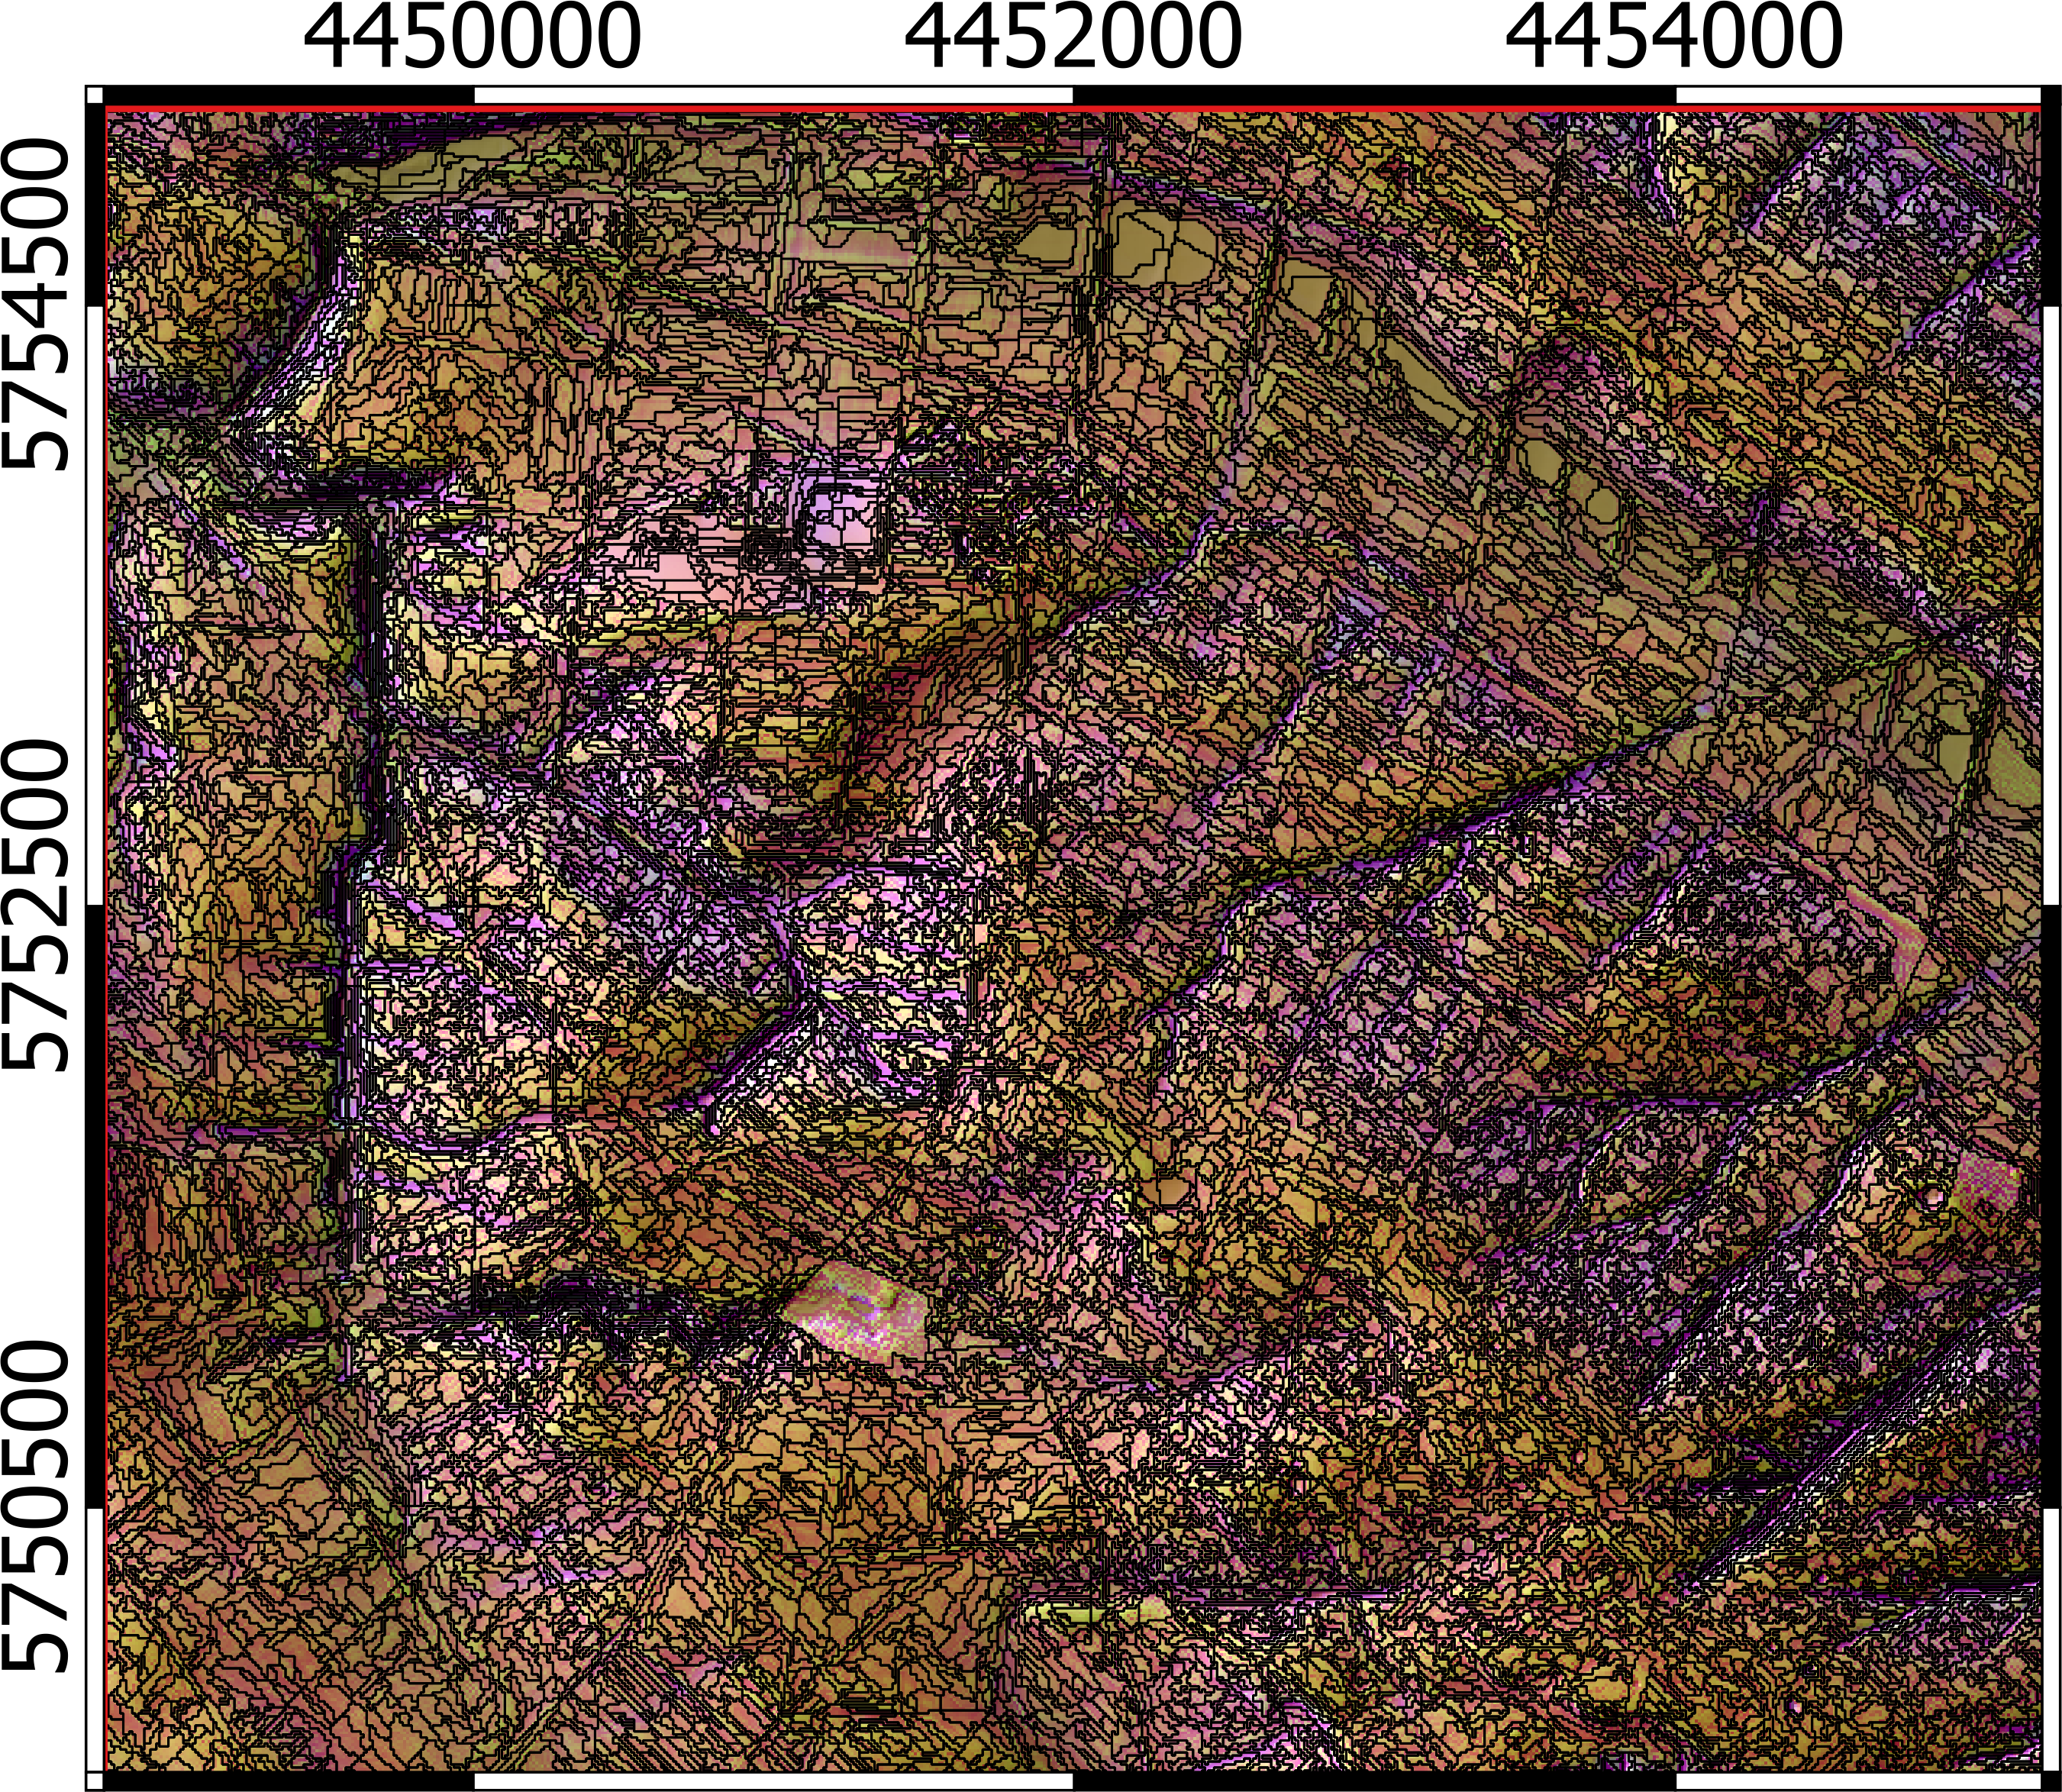
\includegraphics[width=0.48\textwidth]{figures/ReliefobjekteB3}}

\caption[Beispiele für Bezugseinheiten visualisiert anhand eines Bildausschnittes im Testgebiet \textit{Bode}.]{Beispiele für Bezugseinheiten visualisiert anhand eines Bildausschnittes im Testgebiet (vgl. Abb. \ref{fig:ug}b): Ergebnis der Verschneidung von Geologischer Karte 1:25\,000 (GK\,25), Bodenschätzung (BS) und Forstlicher Standortkartierung (FSK; a) sowie Ergebnis der Segmentierung der Reliefattribute \textit{Höhe über Tiefenlienie}, \textit{Massenbilanzindex} und \textit{Neigung} unter Berücksichtigung des Verschneidungsergebnisses von GK\,25, FSK und BS (b)}\label{fig:be}
\end{figure}


Die Zuordnung der Zielmerkmale auf die Bezugseinheiten geschieht unter Zuhilfenahme räumlicher Abfragen auf Datenbankebene (PostgreSQL mit PostGIS). Bei der eigentlichen Attributzuweisung werden zwei Fälle unterschieden: 


\begin{enumerate}
\item Das Verschneidungsergebnis aus Bezugseinsheit und Polygon des Eingangsdatensatzes ergibt eine Ein-zu-eins-Relation. Dann kann das Zielmerkmal eindeutig zugewiesen werden.
\item Wenn das Verschneidungsergebnis keine eindeutige Zuweisung erlaubt, wird eine Wichtungsfunktion angewendet, die den Flächenanteil der zerlegten Schichtinformationen innerhalb der Segmente berücksichtigt und die Zielmerkmale des dominierenden Polygons zuordnet.
\end{enumerate}
%
Als Ergebnis sind zwei Merkmalsausprägungen möglich:

\begin{enumerate}
\item Die Zielmerkmale können qualitative Information darüber enthalten, ob ein spezifischen Zielmerkmal in einer Bezugseinheit auftritt oder nicht. Die beiden Optionen werden durch 1 und 0 kodiert. Tabelle \ref{tab:trans-gen} zeigt für den Kontrollpunkt 207042 (vgl. Abb. \ref{fig:ug}b) die bereits gewichteten Transformationsergebnisse (vgl. Tab. \ref{tab:daten}, S. \pageref{tab:daten}) der Genesemerkmale \textit{g}, \textit{p} und \textit{pfl} (*\_gen\_*-Spalten). In den Beispieldatensätzen enthalten die Datensätze der VBK\,50 (v), FSK (f) und der GK\,25 (g) Informationen der Zielmerkmale. Da das Polygon keinen landwirtschaftlich genutzten Standort repräsentiert, fehlen Angaben der Bodenschätzung (bs). Weiterhin geht aus der Tabelle hervor, dass die FSK und VBK\,50 für die Beispielobjekte nur Geneseangaben bis in eine Tiefe von 12\,dm vorhalten. Ab 13\,dm basiert die Geneseklassifikation ausschließlich auf Merkmalen der GK\,25. 

\begin{sidewaystable}[p]
  \centering
  \caption[Gewichtete Geneseklassen, Klassifikationen mit den höchsten Wichtungen, Anzahl von widersprüchlichen Klassifikationen, korrespondierenden Qualitätsmaße, Klassifikationsquelle sowie die finale Klassifikation für alle Schichten des Kontrollpunktes 207042.]{Gewichtete Geneseklassen (*\_gen\_*), Klassifikationen mit den höchsten Wichtungen (CL\_*), Anzahl von widersprüchlichen Klassifikationen (N\_*),  die korrespondierenden Qualitätsmaße (MS1, MS2, N, STB), die Klassifikationsquelle (SRC) sowie die finale Klassifikation (CLASS) für alle Schichten des Kontrollpunktes 207042 (Abb. \ref{fig:class_final}c u. \ref{fig:GENESE-schicht1-qm}; v -- Vorläufige Bodenkarte 1:50\,000 $|$ g -- Geologische Karte 1:25\,000 $|$ f -- Forstliche Standortskartierung $|$  b -- Bodenschätzung, $|$ m -- Mittelmaßstäbige Landwirtschaftliche Standortskartierung).}\label{tab:trans-gen}
	\vspace*{6pt}
    \begin{tabular8}{r|r|r|r|r|r|r|r|r|r|r|r|r|r|r|r|r|r|r|r|r|r|r}
    \toprule
    \begin{sideways}\textbf{Schicht}\end{sideways} & \begin{sideways}\textbf{v\_gen\_g}\end{sideways} & \begin{sideways}\textbf{v\_gen\_p}\end{sideways} & \begin{sideways}\textbf{v\_gen\_pfl}\end{sideways} & \begin{sideways}\textbf{f\_gen\_g}\end{sideways} & \begin{sideways}\textbf{f\_gen\_p}\end{sideways} & \begin{sideways}\textbf{f\_gen\_pfl}\end{sideways} & \begin{sideways}\textbf{gk\_gen\_g}\end{sideways} & \begin{sideways}\textbf{gk\_gen\_os}\end{sideways} & \begin{sideways}\textbf{gk\_gen\_p}\end{sideways} & \begin{sideways}\textbf{gk\_gen\_pfl}\end{sideways} & \begin{sideways}\textbf{CL\_g}\end{sideways} & \begin{sideways}\textbf{N\_g}\end{sideways} & \begin{sideways}\textbf{CL\_p}\end{sideways} & \begin{sideways}\textbf{N\_p}\end{sideways} & \begin{sideways}\textbf{CL\_pfl}\end{sideways} & \begin{sideways}\textbf{N\_pfl}\end{sideways} & \begin{sideways}\textbf{CLASS}\end{sideways} & \begin{sideways}\textbf{CLASS\_MS1}\end{sideways} & \begin{sideways}\textbf{CLASS\_SUM}\end{sideways} & \begin{sideways}\textbf{CLASS\_N}\end{sideways} & \begin{sideways}\textbf{CLASS\_STB}\end{sideways} & \begin{sideways}\textbf{SOURCE}\end{sideways} \\
    \midrule
    1     & 0     & 0,5   & 0     & 0     & 1     & 0     & 0     & 0     & 0,8   & 0     & 0     & 0     & 1     & 3     & 0     & 0     & p     & 1     & 1     & 1     & 1     & bs,f \\
    \midrule
    2     & 0     & 0,5   & 0     & 0     & 1     & 0     & 0     & 0     & 0,8   & 0     & 0     & 0     & 1     & 3     & 0     & 0     & p     & 1     & 1     & 1     & 1     & bs,f \\
    \midrule
    3     & 0     & 0,5   & 0     & 0     & 1     & 0     & 0     & 0     & 0,8   & 0     & 0     & 0     & 1     & 3     & 0     & 0     & p     & 1     & 1     & 1     & 1     & bs,f \\
    \midrule
    4     & 0     & 0,5   & 0     & 0     & 1     & 0     & 0     & 0     & 0,8   & 0     & 0     & 0     & 1     & 3     & 0     & 0     & p     & 1     & 1     & 1     & 1     & bs,f \\
    \midrule
    5     & 0     & 0,5   & 0     & 0     & 1     & 0     & 0     & 0     & 0,8   & 0     & 0     & 0     & 1     & 3     & 0     & 0     & p     & 1     & 1     & 1     & 1     & bs,f \\
    \midrule
    6     & 0     & 0,5   & 0     & 0     & 1     & 0     & 0     & 0     & 0,8   & 0     & 0     & 0     & 1     & 3     & 0     & 0     & p     & 1     & 1     & 1     & 1     & bs,f \\
    \midrule
    7     & 0     & 0,5   & 0     & 0     & 1     & 0     & 0     & 0     & 0,8   & 0     & 0     & 0     & 1     & 3     & 0     & 0     & p     & 1     & 1     & 1     & 1     & bs,f \\
    \midrule
    8     & 0     & 0,5   & 0     & 0     & 1     & 0     & 0     & 0     & 0,8   & 0     & 0     & 0     & 1     & 3     & 0     & 0     & p     & 1     & 1     & 1     & 1     & bs,f \\
    \midrule
    9     & 0     & 0,5   & 0     & 0     & 1     & 0     & 0     & 0     & 0,8   & 0     & 0     & 0     & 1     & 3     & 0     & 0     & p     & 1     & 1     & 1     & 1     & bs,f \\
    \midrule
    10    & 0     & 0,5   & 0     & 0     & 1     & 0     & 0     & 0     & 0,8   & 0     & 0     & 0     & 1     & 3     & 0     & 0     & p     & 1     & 1     & 1     & 1     & bs,f \\
    \midrule
    11    & 0     & 0,5   & 0     & 0     & 1     & 0     & 0     & 0     & 0     & 0,8   & 0     & 0     & 1     & 2     & 0,8   & 1     & p     & 1     & 1,8   & 2     & 0,2   & bs,f \\
    \midrule
    12    & 0     & 0,5   & 0     & 0     & 1     & 0     & 0     & 0     & 0     & 0,8   & 0     & 0     & 1     & 2     & 0,8   & 1     & p     & 1     & 1,8   & 2     & 0,2   & bs,f \\
    \midrule
    13    & NA    & NA    & NA    & NA    & NA    & NA    & 0     & 0     & 0     & 0,8   & 0     & 0     & 0     & 0     & 0,8   & 1     & pfl   & 0,8   & 0,8   & 1     & 0,8   & gk \\
    \midrule
    14    & NA    & NA    & NA    & NA    & NA    & NA    & 0     & 0     & 0     & 0,8   & 0     & 0     & 0     & 0     & 0,8   & 1     & pfl   & 0,8   & 0,8   & 1     & 0,8   & gk \\
    \midrule
    15    & NA    & NA    & NA    & NA    & NA    & NA    & 0     & 0     & 0     & 0,8   & 0     & 0     & 0     & 0     & 0,8   & 1     & pfl   & 0,8   & 0,8   & 1     & 0,8   & gk \\
    \midrule
    16    & NA    & NA    & NA    & NA    & NA    & NA    & 0     & 0     & 0     & 0,8   & 0     & 0     & 0     & 0     & 0,8   & 1     & pfl   & 0,8   & 0,8   & 1     & 0,8   & gk \\
    \midrule
    17    & NA    & NA    & NA    & NA    & NA    & NA    & 0     & 0     & 0     & 0,8   & 0     & 0     & 0     & 0     & 0,8   & 1     & pfl   & 0,8   & 0,8   & 1     & 0,8   & gk \\
    \midrule
    18    & NA    & NA    & NA    & NA    & NA    & NA    & 0     & 0     & 0     & 0,8   & 0     & 0     & 0     & 0     & 0,8   & 1     & pfl   & 0,8   & 0,8   & 1     & 0,8   & gk \\
    \midrule
    19    & NA    & NA    & NA    & NA    & NA    & NA    & 0     & 0     & 0     & 0,8   & 0     & 0     & 0     & 0     & 0,8   & 1     & pfl   & 0,8   & 0,8   & 1     & 0,8   & gk \\
    \midrule
    20    & NA    & NA    & NA    & NA    & NA    & NA    & 0,8   & 0     & 0     & 0     & 0,8   & 1     & 0     & 0     & 0     & 0     & g     & 0,8   & 0,8   & 1     & 0,8   & gk \\
    \bottomrule
    \end{tabular8}%
\end{sidewaystable}%


\begin{sidewaystable}[p]
  \centering
  \caption[Zielmerkmale \textit{Ton}  und \textit{Schluff}, Klassifikationen der Bodenartengruppe mit den höchsten Wichtungen, Anzahl von widersprüchlichen Klassifikationen, korrespondierenden Qualitätsmaße, Klassifikationsquelle sowie die finale Klassifikation für alle Schichten des Kontrollpunktes 207042.]{Zielmerkmale \textit{Ton} und \textit{Schluff}, Klassifikationen der Bodenartengruppe mit den höchsten Wichtungen (CL\_*), Anzahl von widersprüchlichen Klassifikationen (N\_*), die korrespondierenden Qualitätsmaße (MS1, MS2, N, STB), die Klassifikationsquelle sowie die finale Klassifikation (CLASS) für alle Schichten des Kontrollpunktes 207042 (Abb. \ref{fig:class_final} u. \ref{fig:BAG-schicht1-qm}; koe -- Körnung $|$ t -- Ton $|$ u -- Schluff $|$ v -- VBK\,50 $|$ g -- GK\,25 $|$ f -- FSK $|$  b -- BS $|$ m -- MMK).}\label{tab:trans-ba}
		\vspace*{6pt}
    \begin{tabular8}{r|r|r|r|r|r|r|r|r|r|r|r|r|r|r|r|r|r|r|r|r|r|r|r|r|r}
    \toprule
    \begin{sideways}\textbf{Schicht}\end{sideways} & \begin{sideways}\textbf{bs\_koe\_u}\end{sideways} & \begin{sideways}\textbf{bs\_koe\_t}\end{sideways} & \begin{sideways}\textbf{m\_koe\_u}\end{sideways} & \begin{sideways}\textbf{m\_koe\_t}\end{sideways} & \begin{sideways}\textbf{v\_koe\_u}\end{sideways} & \begin{sideways}\textbf{v\_koe\_t}\end{sideways} & \begin{sideways}\textbf{f\_koe\_u}\end{sideways} & \begin{sideways}\textbf{f\_koe\_t}\end{sideways} & \begin{sideways}\textbf{gk\_koe\_u}\end{sideways} & \begin{sideways}\textbf{gk\_koe\_t}\end{sideways} & \begin{sideways}\textbf{CL\_sl}\end{sideways} & \begin{sideways}\textbf{N\_sl}\end{sideways} & \begin{sideways}\textbf{CL\_ll}\end{sideways} & \begin{sideways}\textbf{N\_ll}\end{sideways} & \begin{sideways}\textbf{CL\_lu}\end{sideways} & \begin{sideways}\textbf{N\_lu}\end{sideways} & \begin{sideways}\textbf{CL\_tl}\end{sideways} & \begin{sideways}\textbf{N\_tl}\end{sideways} & \begin{sideways}\textbf{CLASS}\end{sideways} & \begin{sideways}\textbf{CLASS\_MS1}\end{sideways} & \begin{sideways}\textbf{CLASS\_MS2}\end{sideways} & \begin{sideways}\textbf{CLASS\_SUM}\end{sideways} & \begin{sideways}\textbf{CLASS\_N}\end{sideways} & \begin{sideways}\textbf{CLASS\_STB}\end{sideways} & \begin{sideways}\textbf{SOURCE}\end{sideways} \\
    \midrule
    1     & NA    & NA    & 25    & 14    & 75    & 15    & 75    & 15    & 75    & 15    & 0,2   & 1     & 0     & 0     & 1     & 2     & 0     & 0     & lu    & 1     & 0,2   & 1,2   & 2     & 0,8   & bs,f \\
    \midrule
    2     & NA    & NA    & 25    & 14    & 75    & 15    & 75    & 15    & 75    & 15    & 0,2   & 1     & 0     & 0     & 1     & 2     & 0     & 0     & lu    & 1     & 0,2   & 1,2   & 2     & 0,8   & bs,f \\
    \midrule
    3     & NA    & NA    & 25    & 14    & 75    & 15    & 75    & 15    & 75    & 15    & 0,2   & 1     & 0     & 0     & 1     & 2     & 0     & 0     & lu    & 1     & 0,2   & 1,2   & 2     & 0,8   & bs,f \\
    \midrule
    4     & NA    & NA    & 25    & 14    & 75    & 15    & 75    & 15    & 75    & 15    & 0,2   & 1     & 0     & 0     & 1     & 2     & 0     & 0     & lu    & 1     & 0,2   & 1,2   & 2     & 0,8   & bs,f \\
    \midrule
    5     & NA    & NA    & 25    & 14    & 75    & 15    & 75    & 15    & 75    & 15    & 0,2   & 1     & 0     & 0     & 1     & 2     & 0     & 0     & lu    & 1     & 0,2   & 1,2   & 2     & 0,8   & bs,f \\
    \midrule
    6     & NA    & NA    & 25    & 24    & 75    & 15    & NA    & NA    & 75    & 15    & 0     & 0     & 0,2   & 1     & 0,5   & 1     & 0     & 0     & lu    & 0,5   & 0,2   & 0,7   & 2     & 0,3   & v \\
    \midrule
    7     & NA    & NA    & 25    & 24    & 75    & 15    & NA    & NA    & 75    & 15    & 0     & 0     & 0,2   & 1     & 0,5   & 1     & 0     & 0     & lu    & 0,5   & 0,2   & 0,7   & 2     & 0,3   & v \\
    \midrule
    8     & NA    & NA    & 25    & 24    & 75    & 15    & NA    & NA    & 75    & 15    & 0     & 0     & 0,2   & 1     & 0,5   & 1     & 0     & 0     & lu    & 0,5   & 0,2   & 0,7   & 2     & 0,3   & v \\
    \midrule
    9     & NA    & NA    & 25    & 24    & 75    & 15    & NA    & NA    & 75    & 15    & 0     & 0     & 0,2   & 1     & 0,5   & 1     & 0     & 0     & lu    & 0,5   & 0,2   & 0,7   & 2     & 0,3   & v \\
    \midrule
    10    & NA    & NA    & 25    & 24    & 75    & 15    & NA    & NA    & 75    & 15    & 0     & 0     & 0,2   & 1     & 0,5   & 1     & 0     & 0     & lu    & 0,5   & 0,2   & 0,7   & 2     & 0,3   & v \\
    \midrule
    11    & NA    & NA    & 25    & 14    & 75    & 15    & NA    & NA    & 25    & 27    & 0,2   & 1     & 0     & 0     & 0,5   & 1     & 0,8   & 1     & tl    & 0,8   & 0,5   & 1,5   & 3     & 0,3   & gk \\
    \midrule
    12    & NA    & NA    & 25    & 14    & 75    & 15    & NA    & NA    & 25    & 27    & 0,2   & 1     & 0     & 0     & 0,5   & 1     & 0,8   & 1     & tl    & 0,8   & 0,5   & 1,5   & 3     & 0,3   & gk \\
    \midrule
    13    & NA    & NA    & NA    & NA    & NA    & NA    & NA    & NA    & 25    & 27    & 0     & 0     & 0     & 0     & 0     & 0     & 0,8   & 1     & tl    & 0,8   & 0     & 0,8   & 1     & 0,8   & gk \\
    \midrule
    14    & NA    & NA    & NA    & NA    & NA    & NA    & NA    & NA    & 25    & 27    & 0     & 0     & 0     & 0     & 0     & 0     & 0,8   & 1     & tl    & 0,8   & 0     & 0,8   & 1     & 0,8   & gk \\
    \midrule
    15    & NA    & NA    & NA    & NA    & NA    & NA    & NA    & NA    & 25    & 27    & 0     & 0     & 0     & 0     & 0     & 0     & 0,8   & 1     & tl    & 0,8   & 0     & 0,8   & 1     & 0,8   & gk \\
    \midrule
    16    & NA    & NA    & NA    & NA    & NA    & NA    & NA    & NA    & 25    & 27    & 0     & 0     & 0     & 0     & 0     & 0     & 0,8   & 1     & tl    & 0,8   & 0     & 0,8   & 1     & 0,8   & gk \\
    \midrule
    17    & NA    & NA    & NA    & NA    & NA    & NA    & NA    & NA    & 25    & 27    & 0     & 0     & 0     & 0     & 0     & 0     & 0,8   & 1     & tl    & 0,8   & 0     & 0,8   & 1     & 0,8   & gk \\
    \midrule
    18    & NA    & NA    & NA    & NA    & NA    & NA    & NA    & NA    & 25    & 27    & 0     & 0     & 0     & 0     & 0     & 0     & 0,8   & 1     & tl    & 0,8   & 0     & 0,8   & 1     & 0,8   & gk \\
    \midrule
    19    & NA    & NA    & NA    & NA    & NA    & NA    & NA    & NA    & 25    & 27    & 0     & 0     & 0     & 0     & 0     & 0     & 0,8   & 1     & tl    & 0,8   & 0     & 0,8   & 1     & 0,8   & gk \\
    \midrule
    20    & NA    & NA    & NA    & NA    & NA    & NA    & NA    & NA    & 25    & 27    & 0     & 0     & 0     & 0     & 0     & 0     & 0,8   & 1     & tl    & 0,8   & 0     & 0,8   & 1     & 0,8   & gk \\
    \bottomrule
    \end{tabular8}%


\end{sidewaystable}%

\item Quantitative Zielmerkmale repräsentieren konkrete Werte, die erst durch eine Klassifikation kategorisiert werden (Kap. \ref{sec:class}). Das betrifft im Rahmen des Projektes die Körnungszielmerkmale \textit{Ton} (t) und \textit{Schluff} (u). Die Struktur der Datei des quantitativen Transformationsergebnisses  wird in Tabelle \ref{tab:trans-ba} veranschaulicht. Dort sind für den Kontrollpunkt 207042 (Abb. \ref{fig:ug}b)  die schichtspezifische Körnungswerte (*\_koe\_*-Spalten) in Abhängigkeit von den Datenquellen aufgelistet. Danach kön"-nen aus der FSK (f), VBK\,50 (v), MMK (m) und GK\,25 (gk) Informationen zur Körnung abgeleitet werden. Die Tabelle macht auch deutlich, dass sich Werte widersprechen können oder sich der vertikale Informationsgehalt in Abhängigkeit von den Datenquellen unterscheidet. Das betrifft beispielsweise die abgeleiteten Schluff- und Tongehalte der Informationsquelle \textit{m}, die deutlich von denen der Informationsquellen \textit{v}, \textit{f} und \textit{gk} abweichen. Weiterhin ist festzustellen, dass Informationen der FSK, MMK bzw. VBK\,50 bis 12\,dm und der GK\,25 bis 20\,dm reichen. 
\end{enumerate}


\subsection{Klassifikation der Bodenartengruppen und Bodengenese}\label{sec:class}
Die schichtspezifische \textit{Klassifikation der quantitativen Zielmerkmale} (\textit{hier:} Bodenartengruppe) gliedert sich in drei Schritte. Bei der \textit{Klassifikation der qualitativen Zielmerkmale} (\textit{hier:} Bodengenese) kommen nur die Schritte zwei und drei zur Anwendung. Die aus der Klassifikation der Bodengenese und Bodenartengruppen resultierenden schichtspezifischen Datensätze sind für den Kontrollpunkt 207042 (Abb. \ref{fig:ug}b) in den Tabellen \ref{tab:trans-gen} und \ref{tab:trans-ba} dokumentiert:


\begin{enumerate}
\item Bei der Gruppierung werden die Körnungsarten \textit{Ton} und \textit{Schluff} entsprechend der Klassifikationsvorschrift in der Bodenkundlichen Kartierunganleitung \citep[S. 144 ff]{KA5} zusammengefasst, wobei zwischen den semantischen Aggregationsniveaus \textit{Bodenart}, \textit{Bodenartengruppe} und \textit{Bodenartenhauptgruppe} gewählt werden kann. Der innerhalb des ProBoSA-Portals editierbare Programmcode ist mit der statistischen Skriptsprache \textbf{R} umgesetzt worden \citep{R2015}. Der Programmcode \ref{prog:bag-su} veranschaulicht die Klassifikationsvorschrift für die Bodenartengruppe \textit{lu}, die für die Klassifikation der Boden"-schätz"-ungs"-in"-for"-mationen (\texttt{b}) anwendbar ist. Danach wird der Spalte \texttt{BAG\_lu\_b} in der Attributtabelle des Schichtdatensatzes \texttt{s@data} der Wichtungsfaktor \texttt{w.b} zugeordnet, wenn die Klassifikationsbedingungen erfüllt sind. Treffen die Bedingungen nicht zu, wird der Wert 0 zugewiesen. Der Wichtungsfaktor ist eine Variable mit dem Wertebereich $w \in [0,1]$, die vom Nutzer definiert wird und die expertenbasierte Datenqualität repräsentiert. Die höchste Datenqualität wird durch den Wert 1, die niedrigste durch den Wert 0 ausgedrückt. Entsprechend Tabelle \ref{tab:daten} werden der Bodenschätzung ($\text{\texttt{w.b}}=1$) und der Forstlichen Standortskartierung  ($\text{\texttt{w.f}}=1$) die höchsten Datenqualitäten zugewiesen. Es folgen die Informationen der Geologischen Karte 1:25\,000 ($\text{\texttt{w.g}}=0,8$), der Vorläufigen Bodenkarte 1:50\,000 ($\text{\texttt{w.v}}=0,5$) und der Mittelmaßstäbigen Standortskartierung ($\text{\texttt{w.m}}=0,2$).


\begin{program}[t] 
\begin{verbatim} 
s@data$BAG_lu_b <- ifelse((s@data$b_koe_t>=8  & s@data$b_koe_t<12  & 
							             s@data$b_koe_u>=65 & s@data$b_koe_u<92) | 
                           (s@data$b_koe_t>=12 & s@data$b_koe_t<17  & 
                           s@data$b_koe_u>=65 & s@data$b_koe_u<88) | 
                           (s@data$b_koe_t>=8  & s@data$b_koe_t<17  & 
                           s@data$b_koe_u>=50 & s@data$b_koe_u<65),
                       w.b,
                       0)
\end{verbatim}
\caption{\textbf{R}-Programmcode zur Klassifikation der Bodenartengruppe \textit{lu} basierend auf Informationen der Bodenschätzung (b).} 
\label{prog:bag-su} 
\end{program} 



Bei der Klassifikation kann definiert werden, welche Informationsquellen pro Schicht verwendet werden. So wird der Bodenartengruppen- bzw. Bodenartenhauptgruppen-Klassifikation der Schichten 1 bis 10 nur die Informationen der Bodenschätzung, MMK, FSK und VBK\,50 berücksichtigt. Ab Schicht 11 fanden auch die Informationen der GK\,25 Eingang in die Klassifikation (vgl. Tab. \ref{tab:trans-ba}).

\item Als Zwischenergebnis der  Klassifikation werden Datensätze generiert, die pro Zielklasse, Bezugseinheit und Schicht alle Zuweisungen der Wichtungsfaktoren zusammenfassen. Danach werden in den \textit{CL\_*}-Spalten die Klassifikationen mit den höchsten Wichtungen aggregiert. Wenn also die Klassifikation mehrerer Datengrundlagen zu einem gleichen Ergebnis führt, wird der höchste Wichtungsfaktor übernommen. Das ist beispielsweise in Tabelle \ref{tab:trans-gen} der Fall, wo das Klassifikationsergebnis der ersten Schicht \textit{p} den Datengrundlagen \textit{v}, \textit{gk} und \textit{f} zugeordnet werden kann. In den \textit{N\_*}-Spalten wird die Anzahl der übereinstimmenden Klassifilationen dokumentiert (hier: 3). Ergibt die Klassifikation verschiedene Ergebnisse, werden in den \textit{CL\_*}-Spalten die korresondierenden Wichtungsfaktoren abgelegt. So führt beispielsweise die Bodenartengruppen-Klassifikation der ersten Schicht zu den beiden Ergebnissen  $\text{\textit{CL\_sl}}=0,2$  und $\text{\textit{CL\_lu}}=1$ (Tab. \ref{tab:trans-ba}).

\item Die finale Klassifikation (Spalte \textit{CLASS}) für jede Bezugseinheit ergibt sich aus dem höchsten Wichtungsfaktor der Spalten \textit{CL\_}*. In Tabelle \ref{tab:trans-ba} wird zum Beispiel die erste Schicht des Kontrollpunkte 207042 als \textit{lu} klassifiziert. Die alternative Klassifikation \textit{sl} ist durch einen geringere Wichtungsfaktor gekennzeichnet.\newline
Neben der finalen Klassifikation wird jede Bezugseinheit und Schicht durch einfache Qualitätsmaße charakterisiert.  Das Maß \textit{MS1} beschreibt den höchsten Wichtungsfaktor des finalen Klassifikationsergebnisses. Der Wichtungsfaktor der zweitbesten Klassifikation wird durch das Maß \textit{MS2} und die Anzahl alternativer Klassifikationen wird durch das Maß \textit{N} ausgedrückt, die Differenz von \textit{MS1} und \textit{MS2} wird als Klassifikationsstbilität \textit{STB} bezeichnet. Für die Klassifikation der ersten Zeile in Tabelle \ref{tab:trans-ba} ergibt sich  ein \textit{MS1}-Wert von 1, da die FSK die Grundlage der Klassifikation bildet. Der $MS2$-Wert von 0,2 weist darauf hin, dass die Klassififkation der MMK zu einem alternativen Ergebnis führte. Aus beiden Werten leitet sich ein \textit{STB}-Wert von 0,8 ab. Der \textit{N}-Wert von 2 besagt, dass zwei alternative Klassifikationen existieren.
\end{enumerate}

\begin{figure}[p]
\subfigure[]{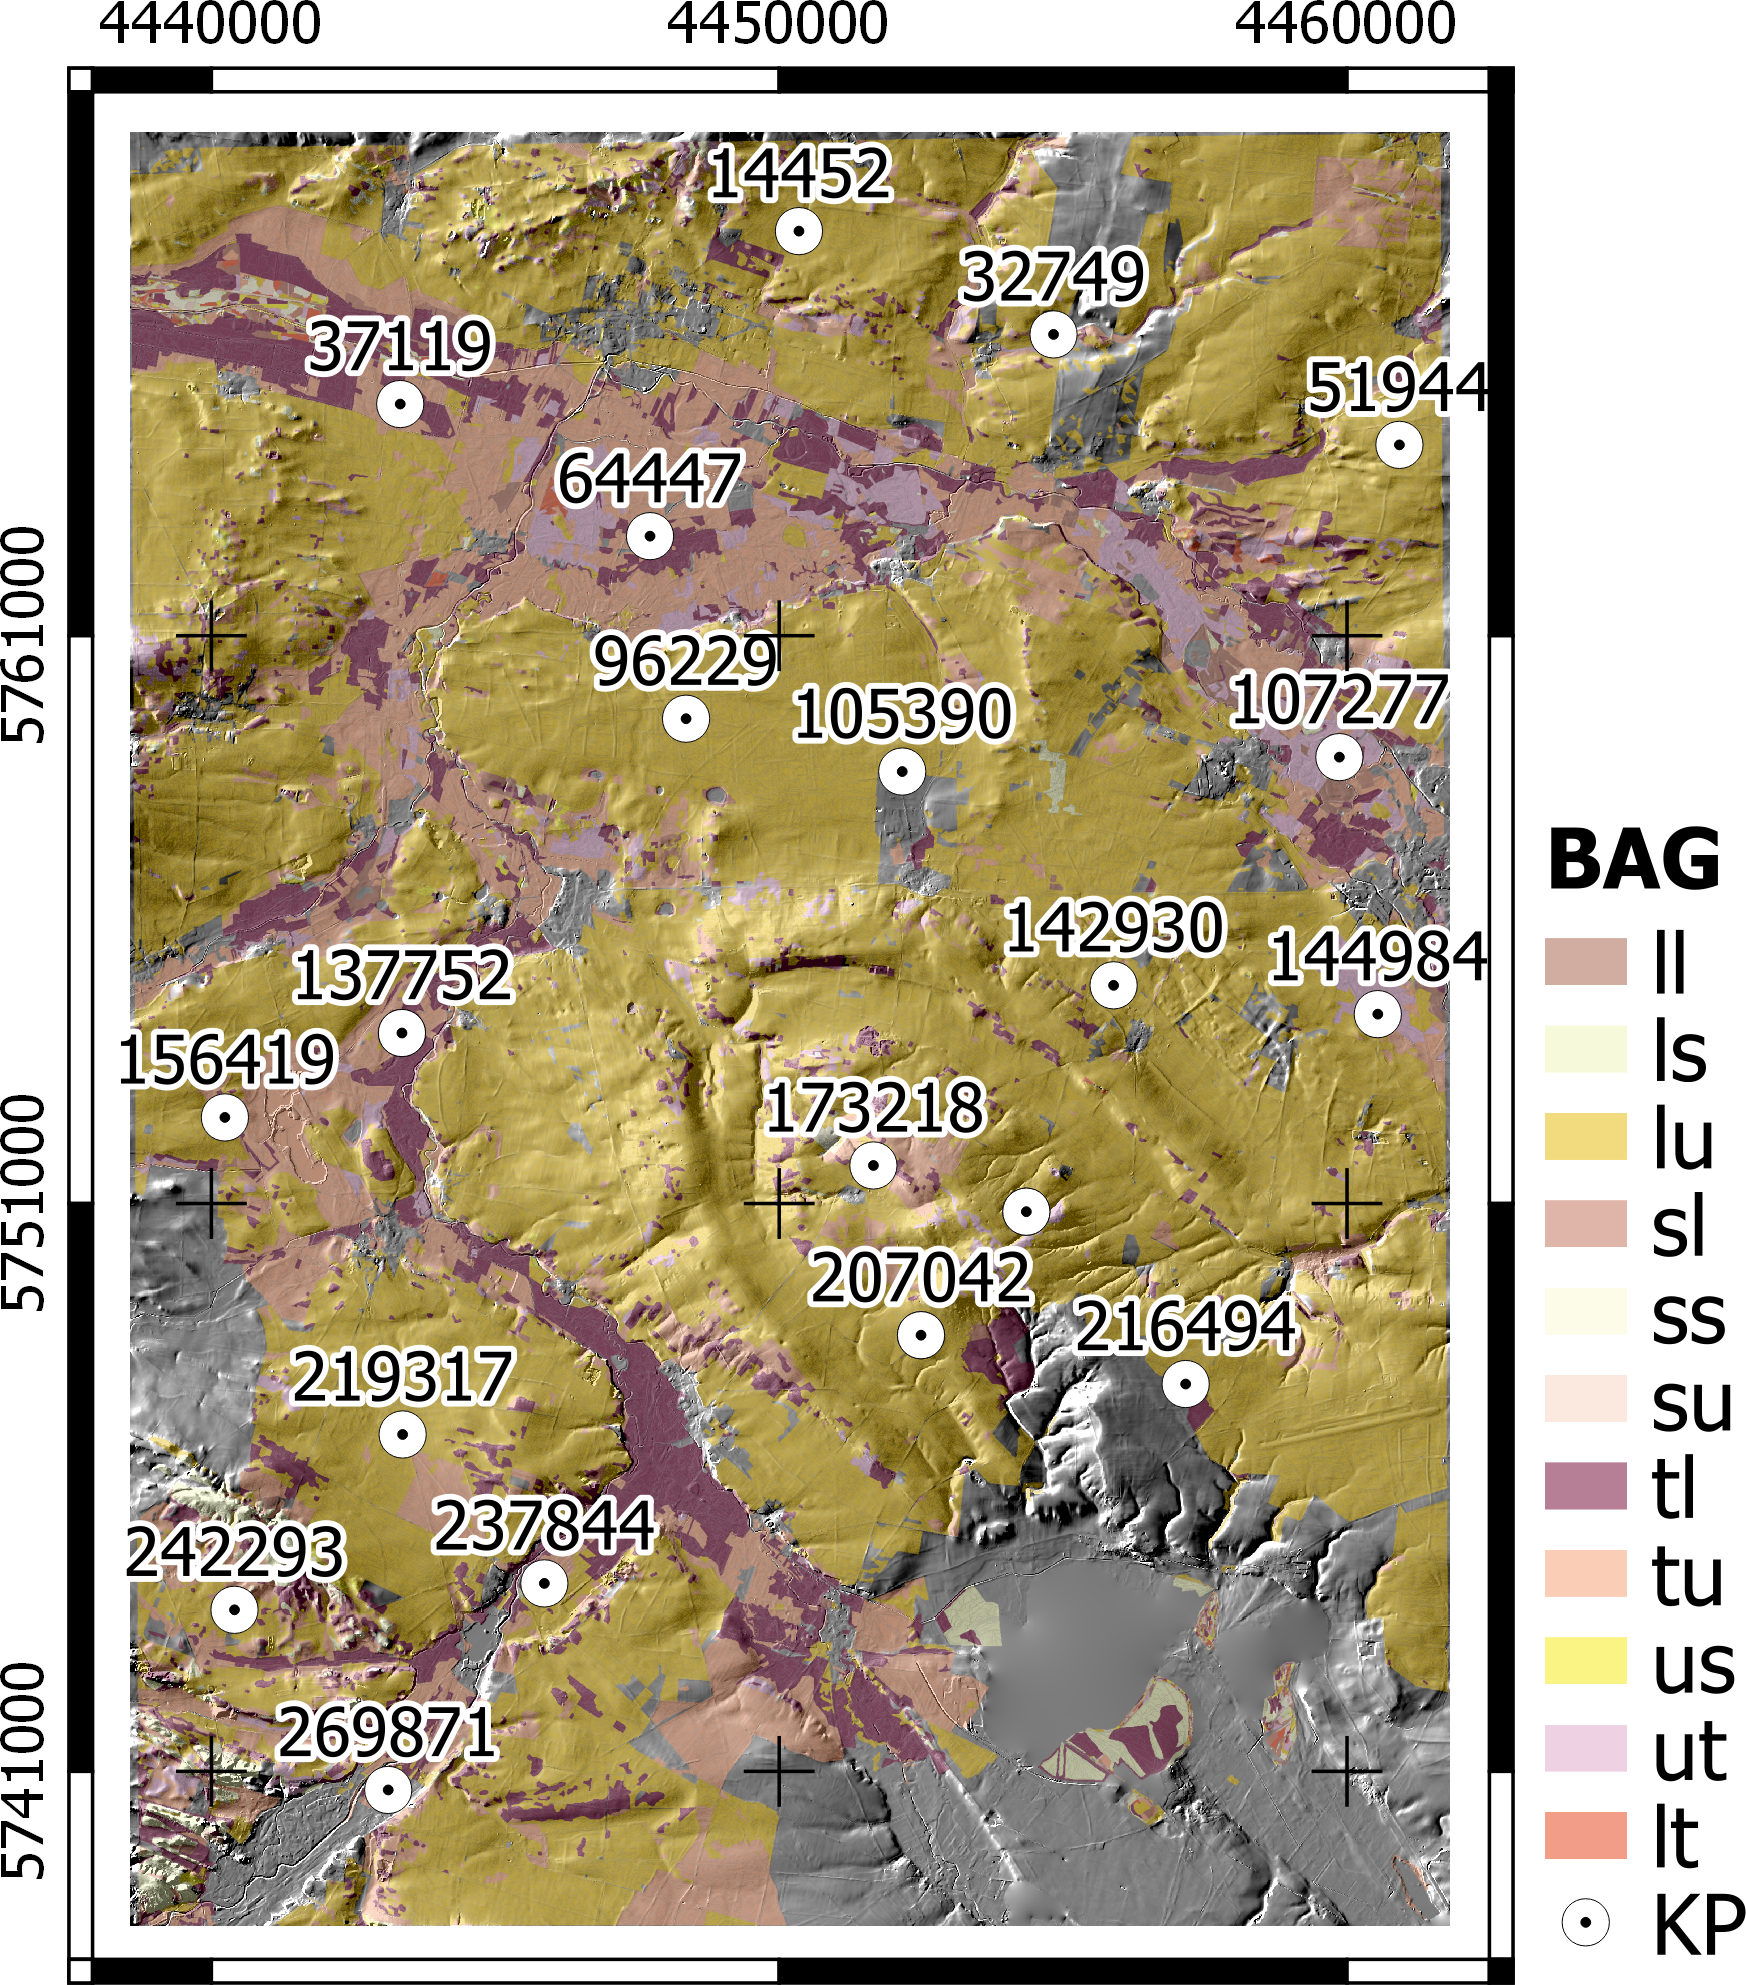
\includegraphics[height=0.48\textwidth]{figures/BAG_Schicht1}}\quad
\subfigure[]{\includegraphics[width=0.48\textwidth]{figures/bezugseinheiten_basic_CLASS_1_BAG_Flaechenanteile.pdf}}

\subfigure[]{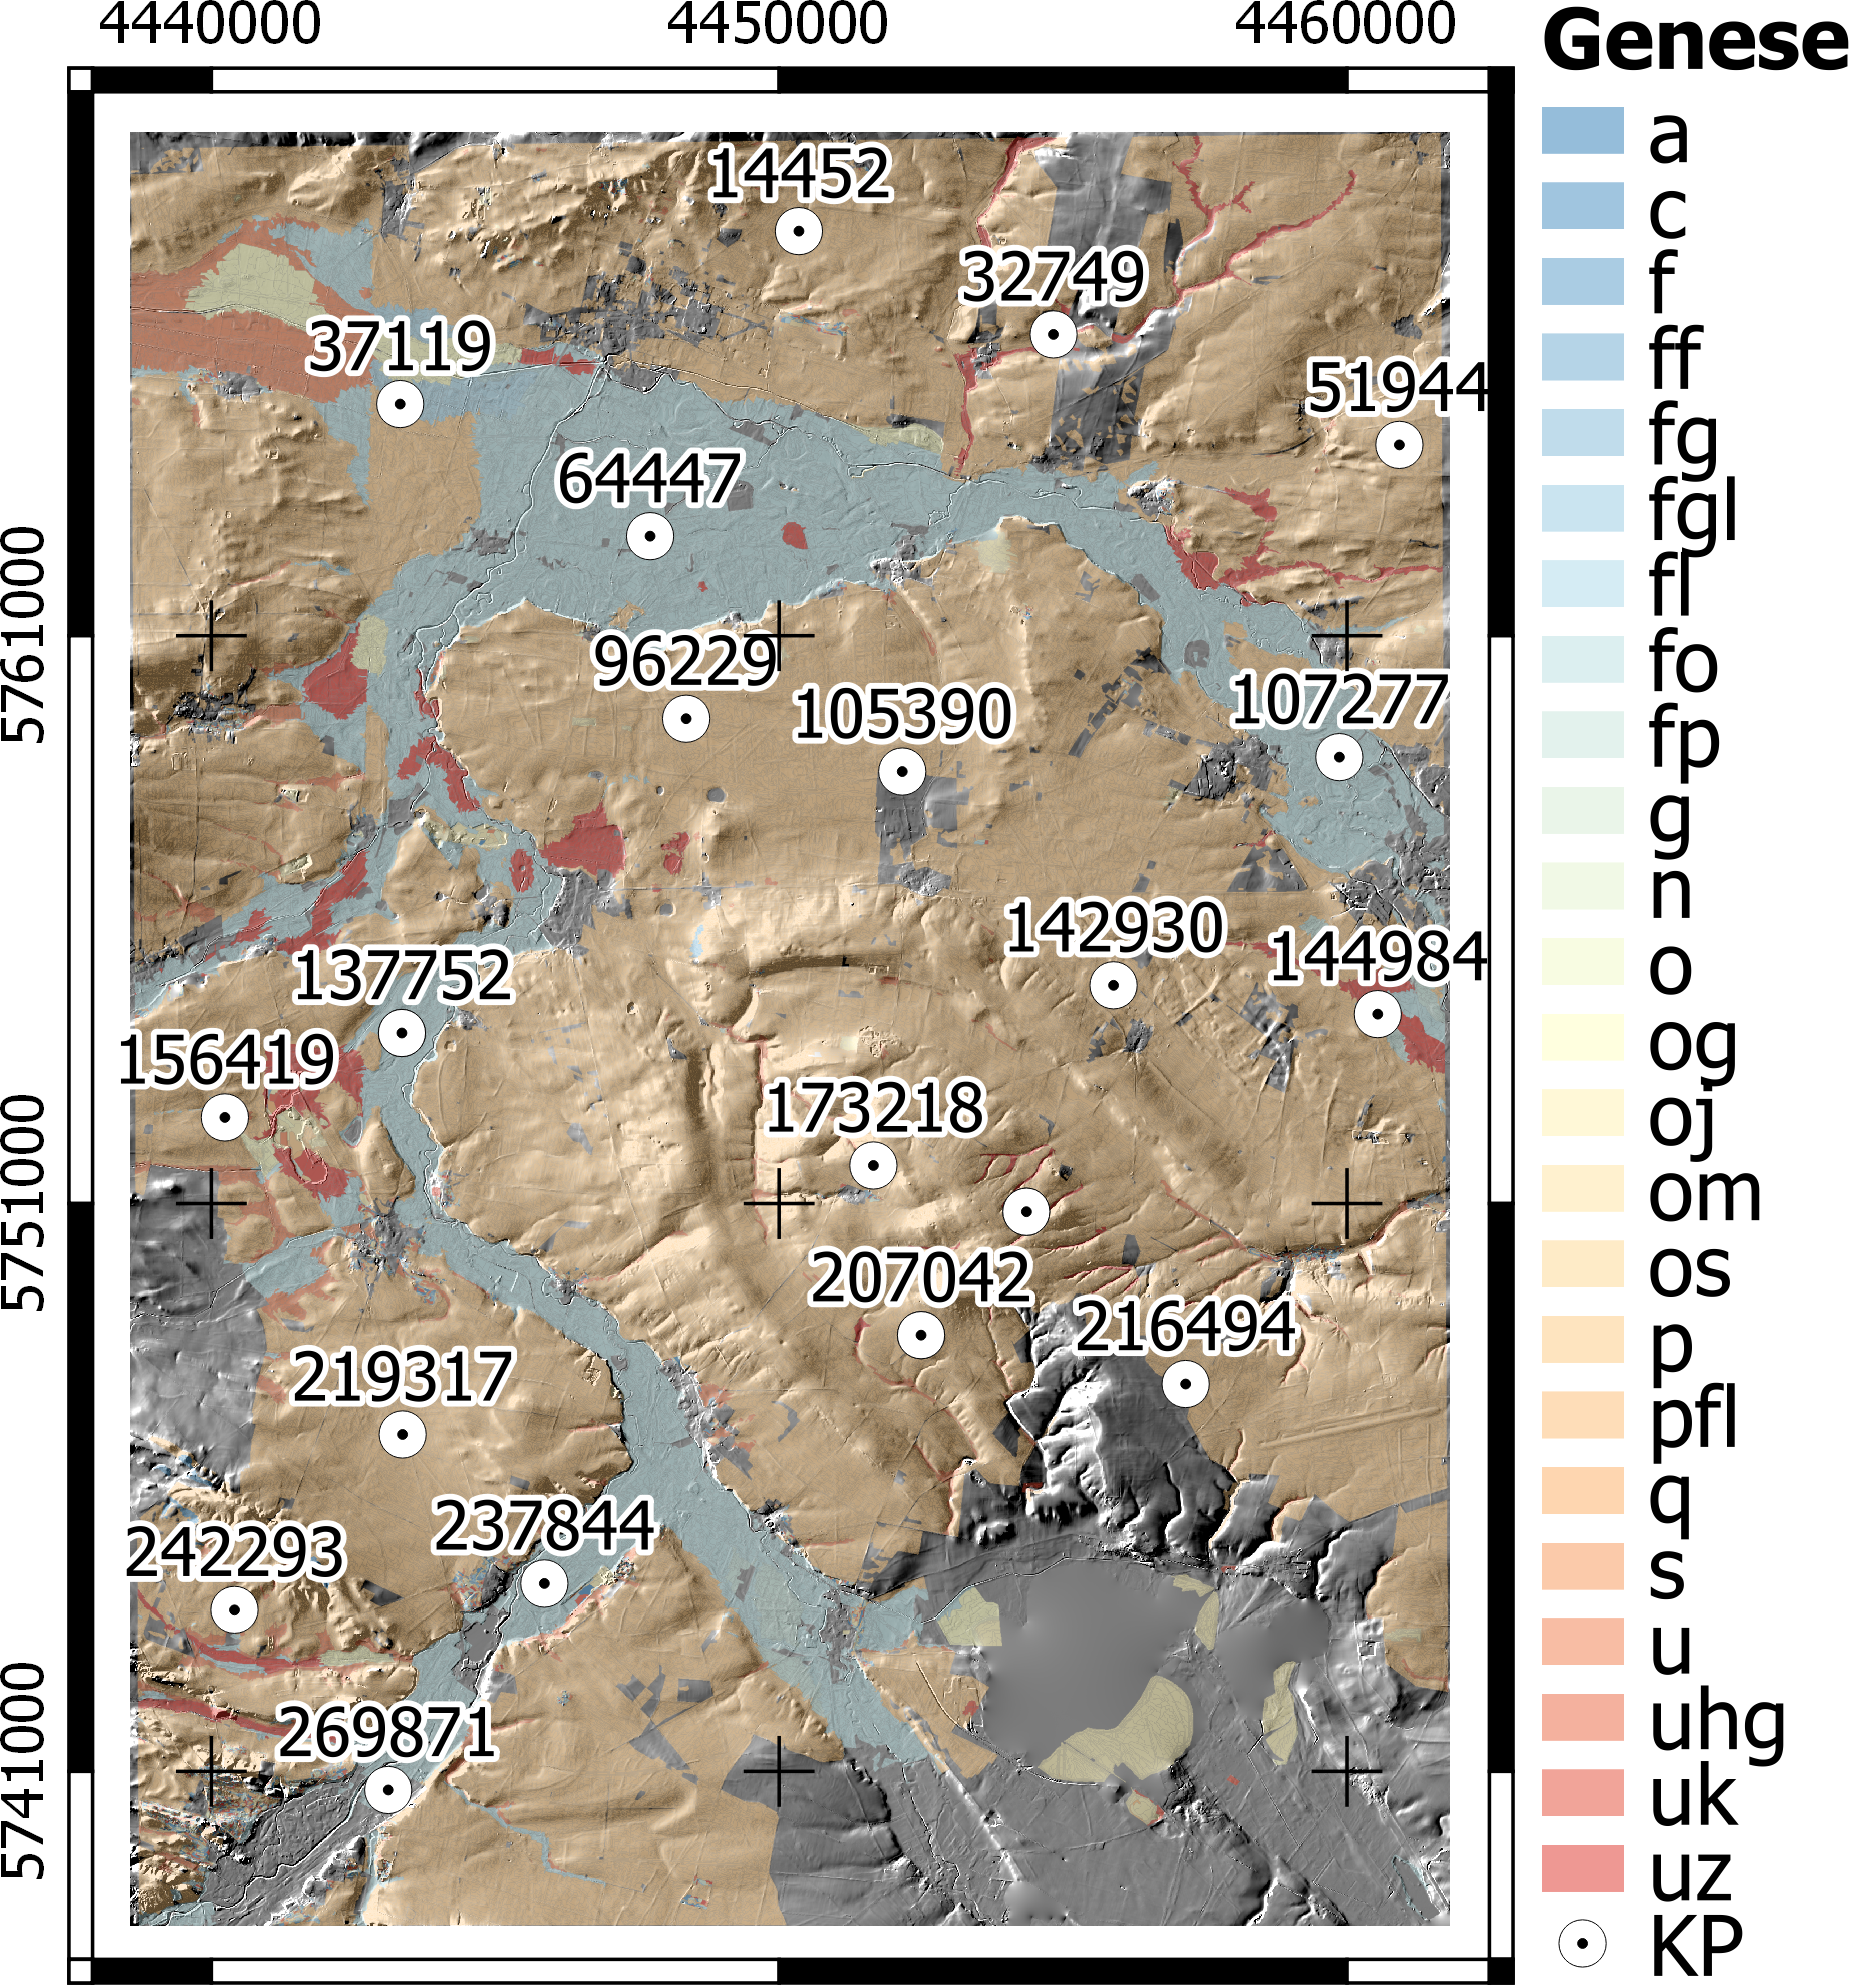
\includegraphics[height=0.48\textwidth]{figures/Genese_Schicht1}}
\subfigure[]{\includegraphics[width=0.48\textwidth]{figures/bezugseinheiten_basic_CLASS_1_GEN_Flaechenanteile.pdf}}
\caption[Klassifikationergebnisse der  Bodenartengruppen und Genese für die Schicht 1 und die korrespondierenden Flächenanteile im Testgebiet \textit{Bode}.]{Klassifikationergebnisse der  Bodenartengruppen (BAG; a) und Genese (c) für die Schicht 1 und die korrespondierenden Flächenanteile (b, d) im Testgebiet \textit{Bode}.}\label{fig:class_final}
\end{figure}


\begin{figure}[p]
\subfigure[MS1]{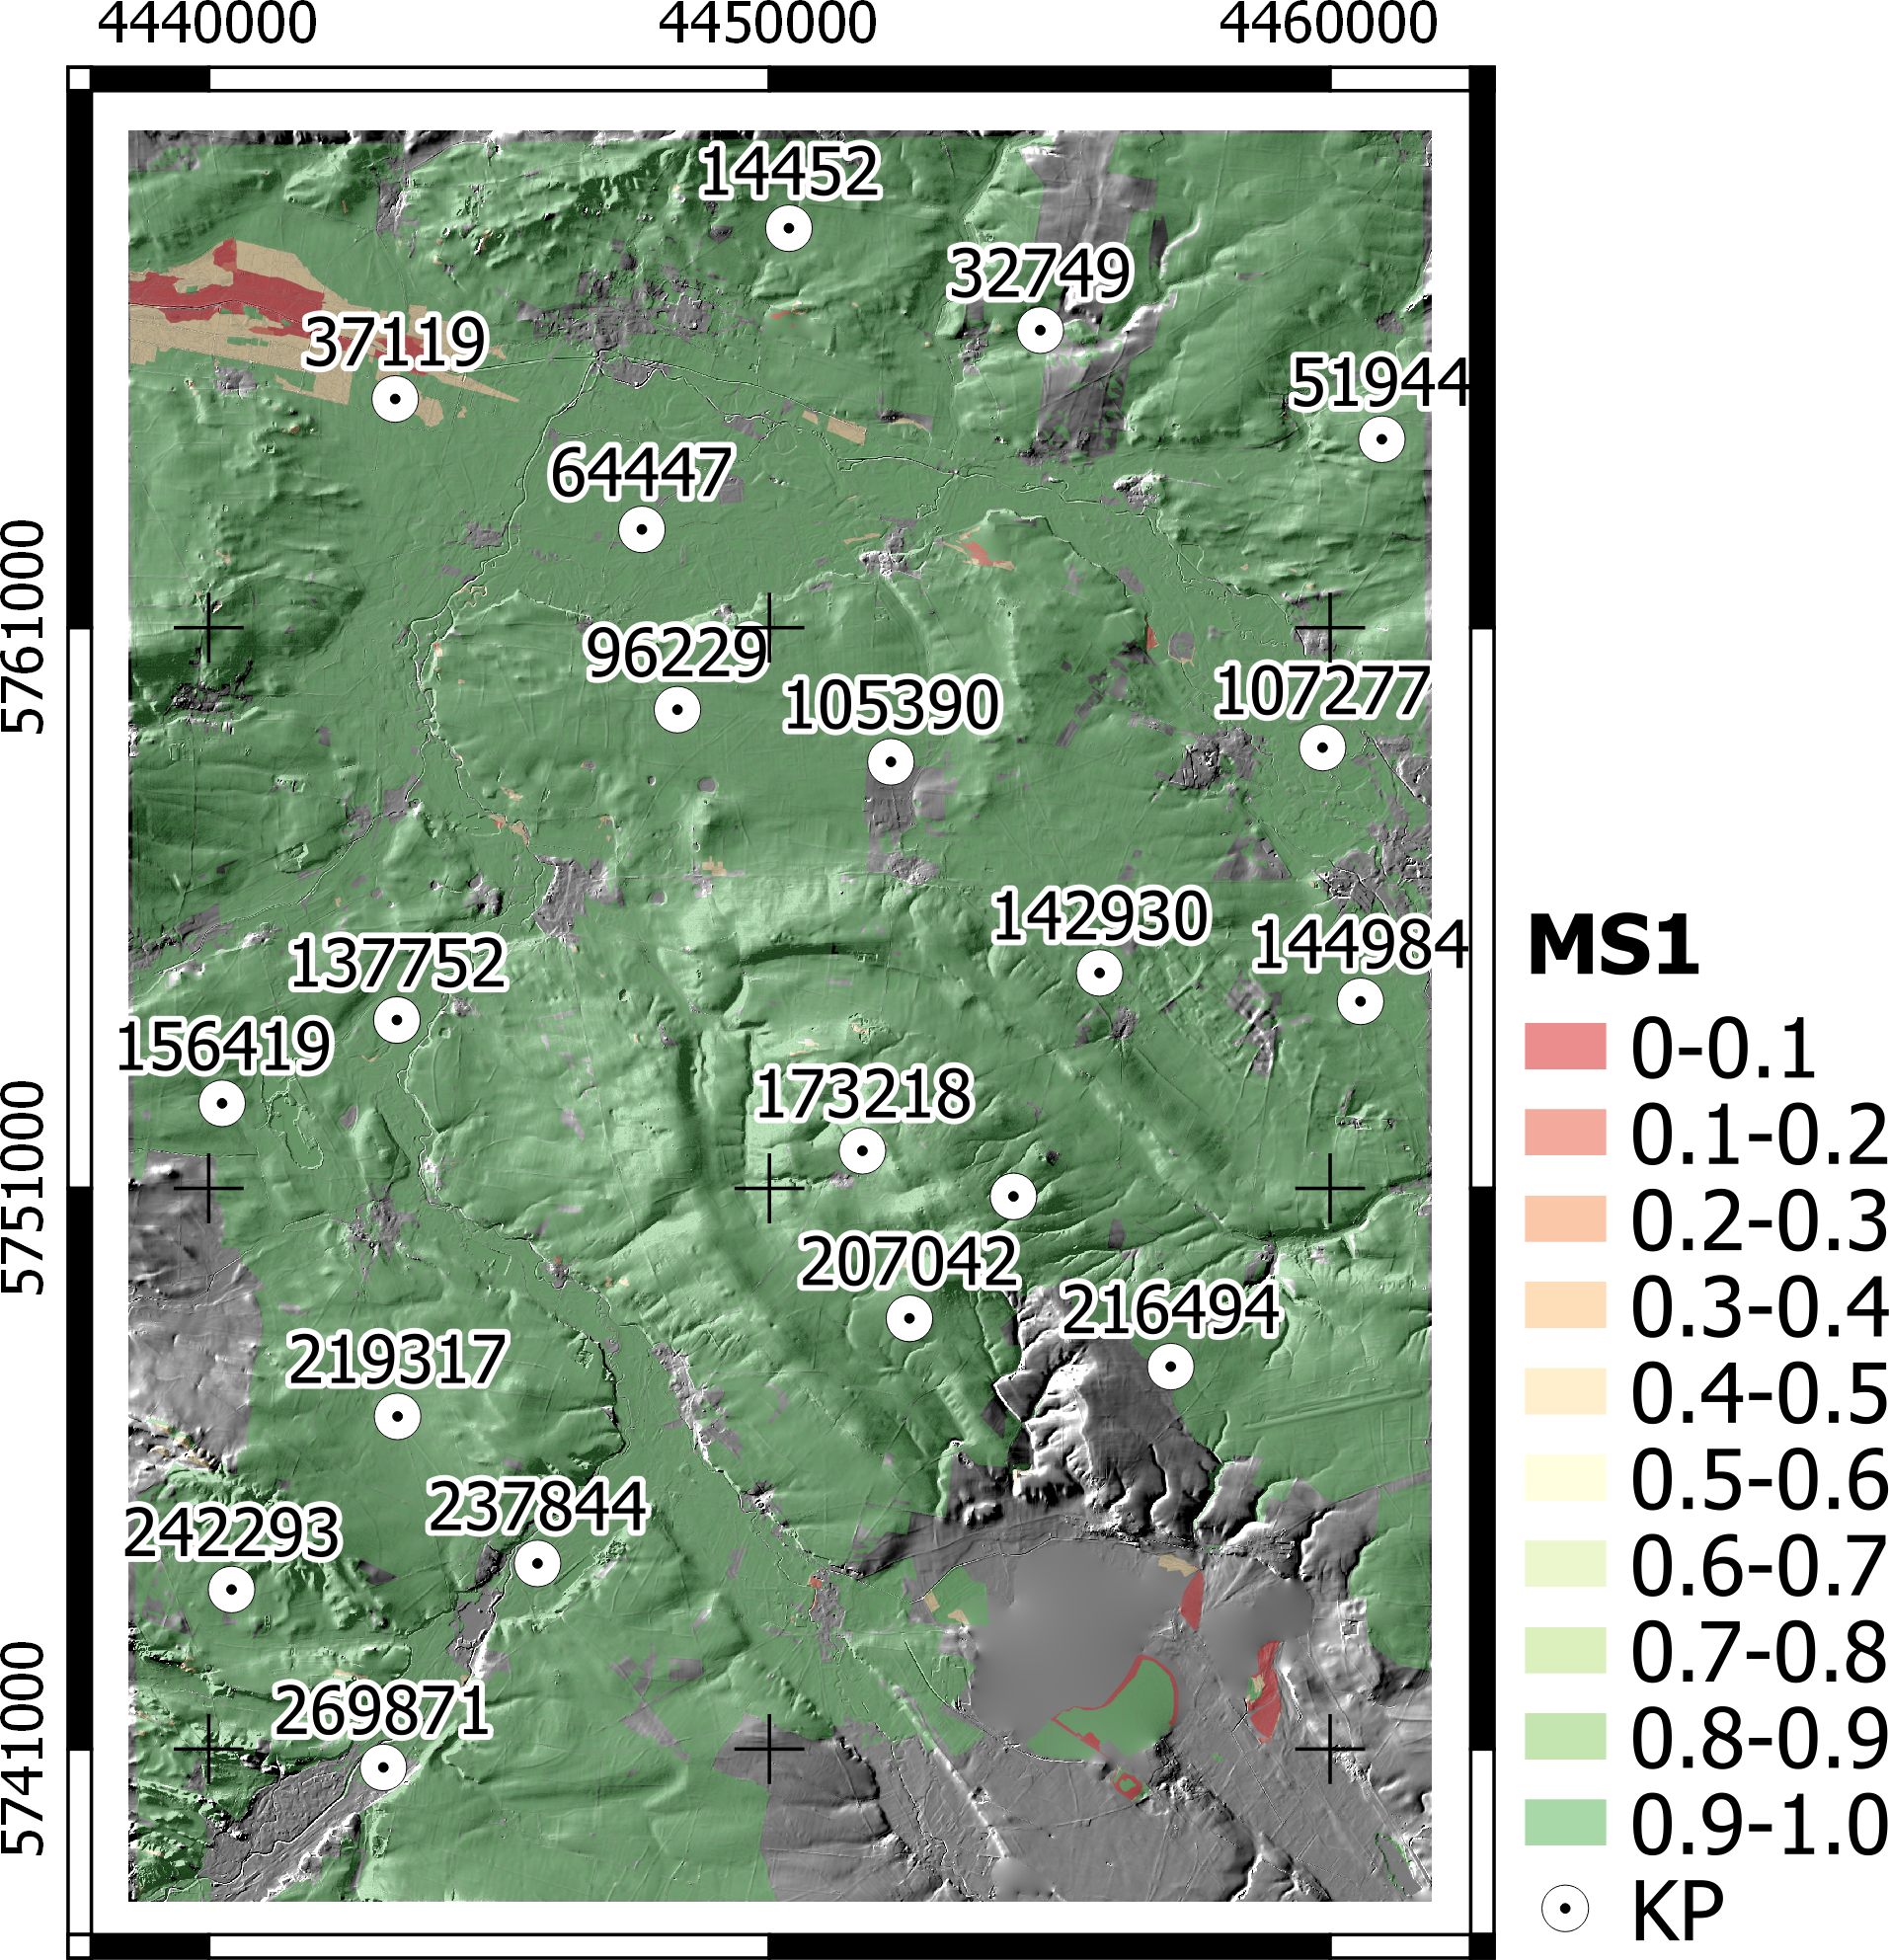
\includegraphics[height=0.48\textwidth]{figures/BAG_Schicht1MS1}}\quad
\subfigure[STB]{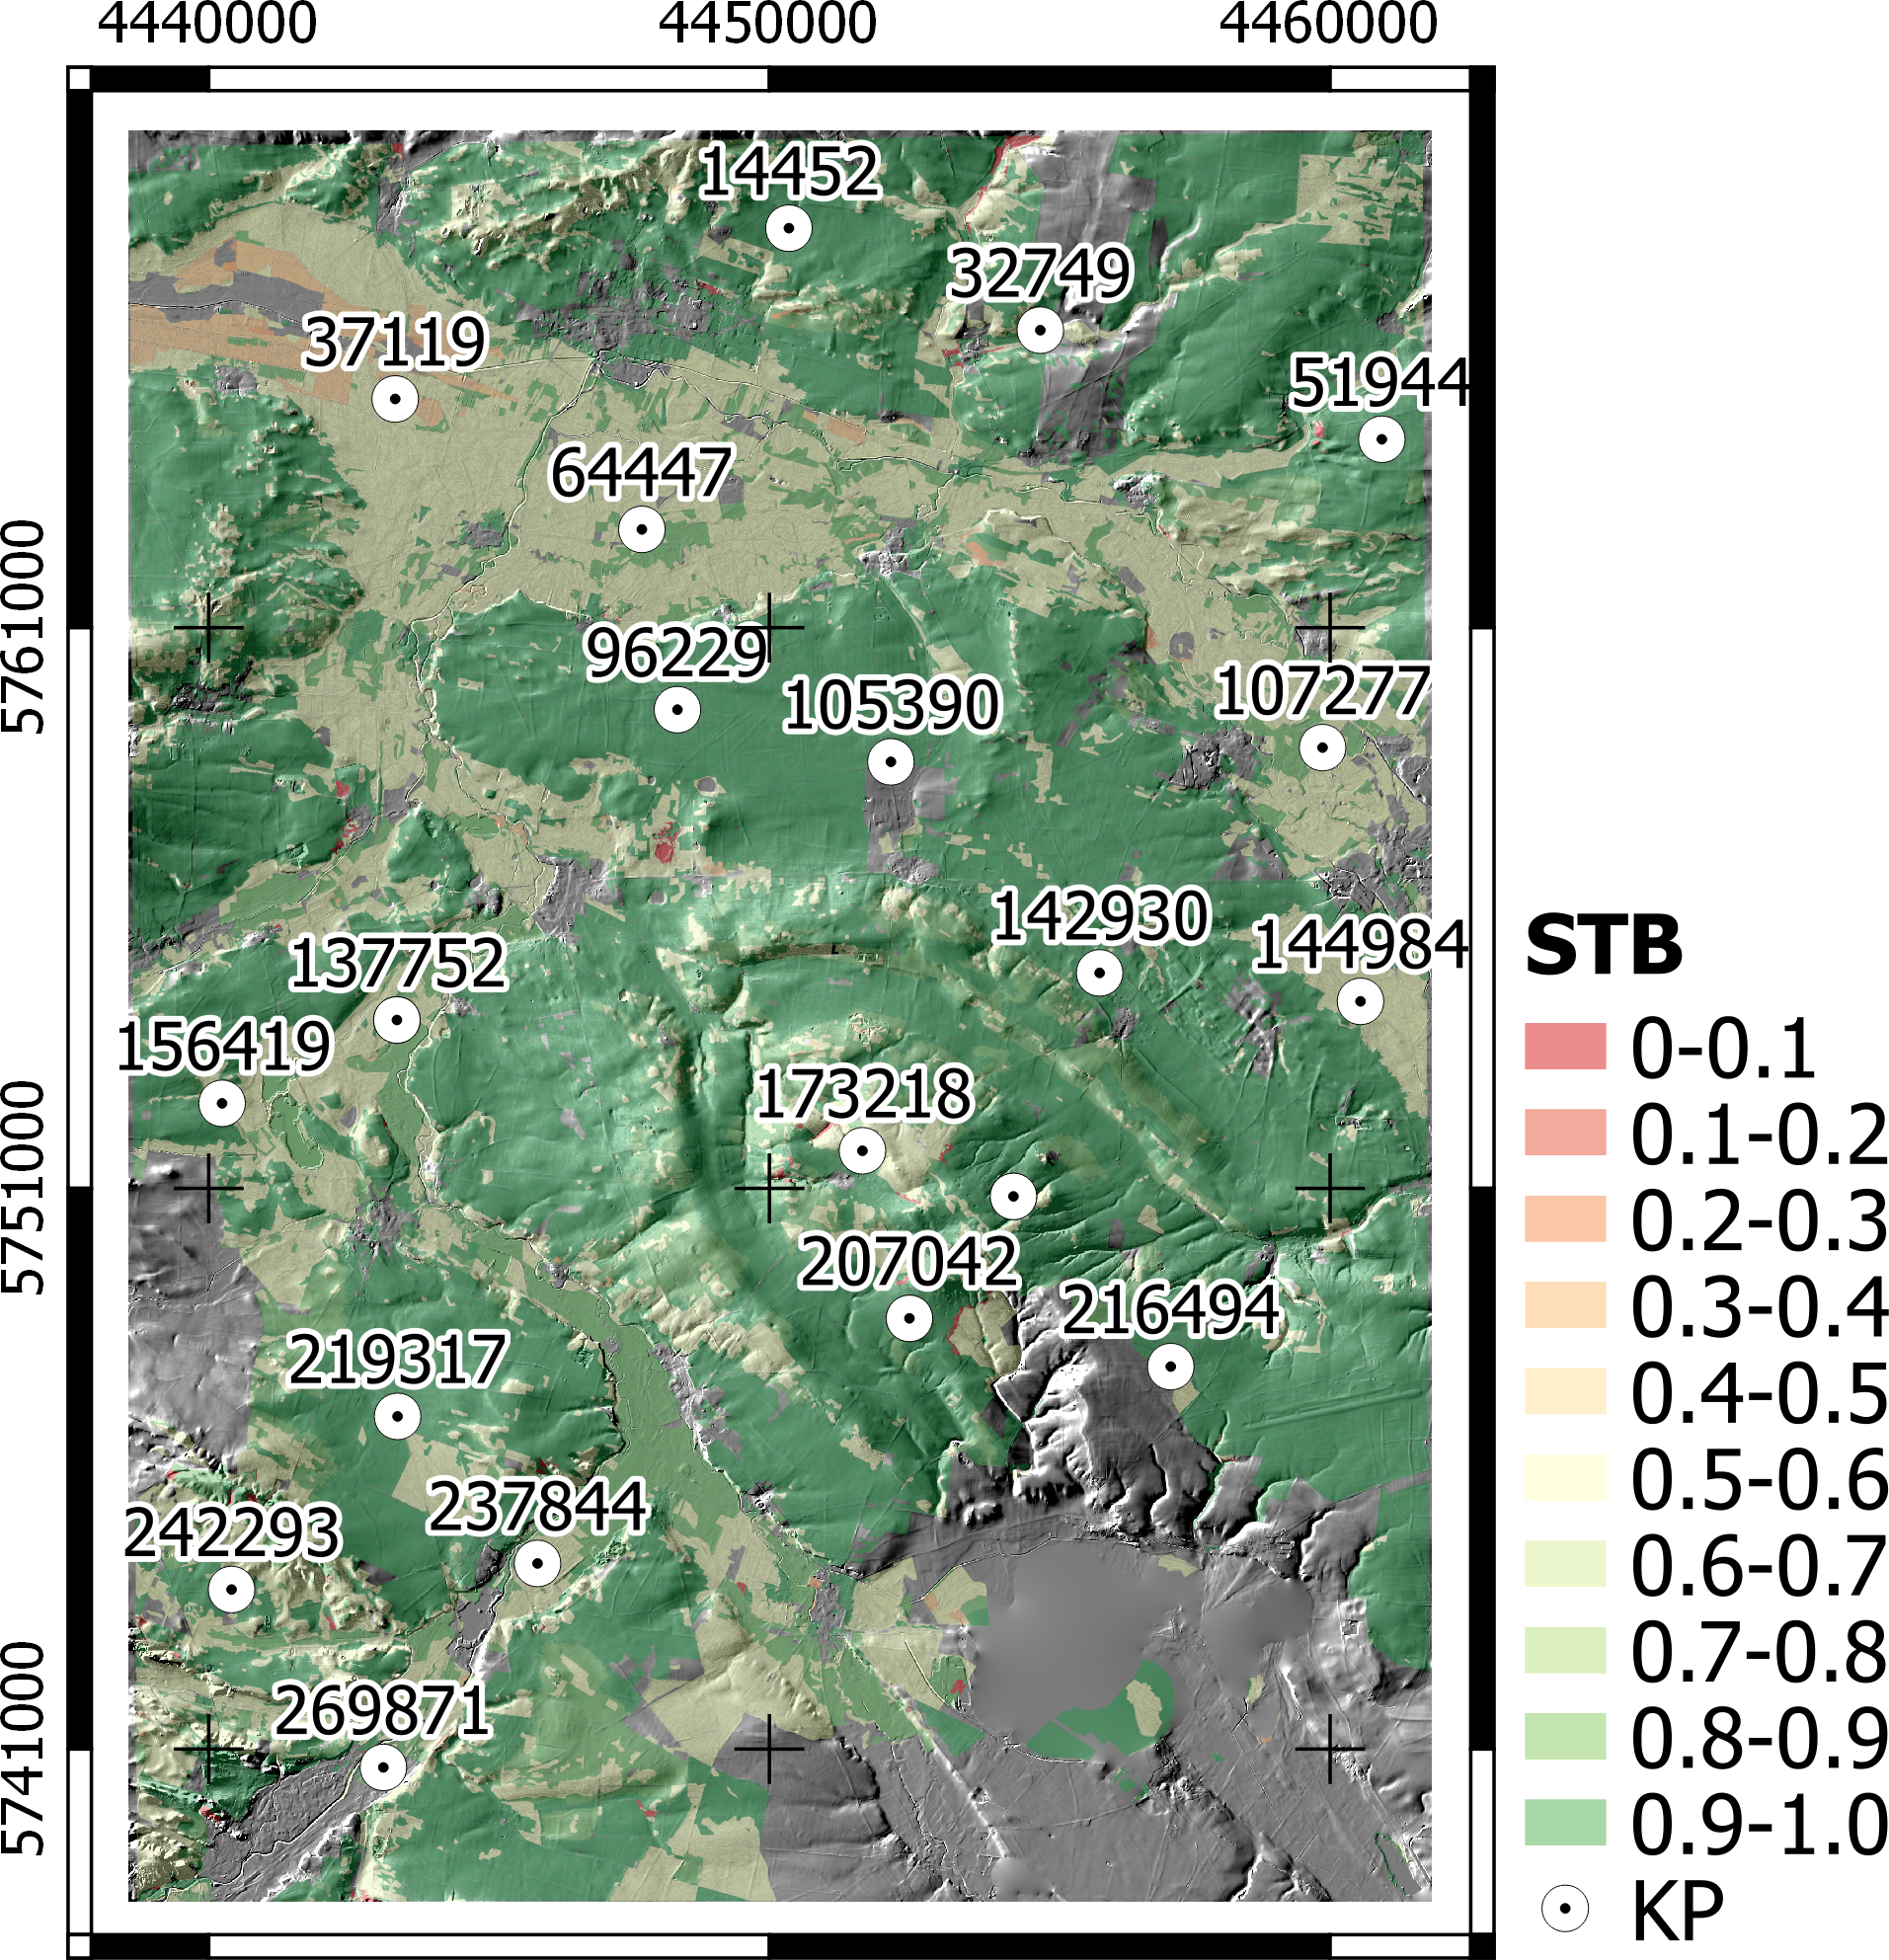
\includegraphics[height=0.48\textwidth]{figures/BAG_Schicht1STB}}\quad
\caption{Qualitätsmaße \textit{MS1} und \textit{STB} für die Bodenartengruppenklassifikation der Schicht 1 im Testgebiet \textit{Bode}.}\label{fig:BAG-schicht1-qm}
\end{figure}

\begin{figure}[p]
\subfigure[MS1]{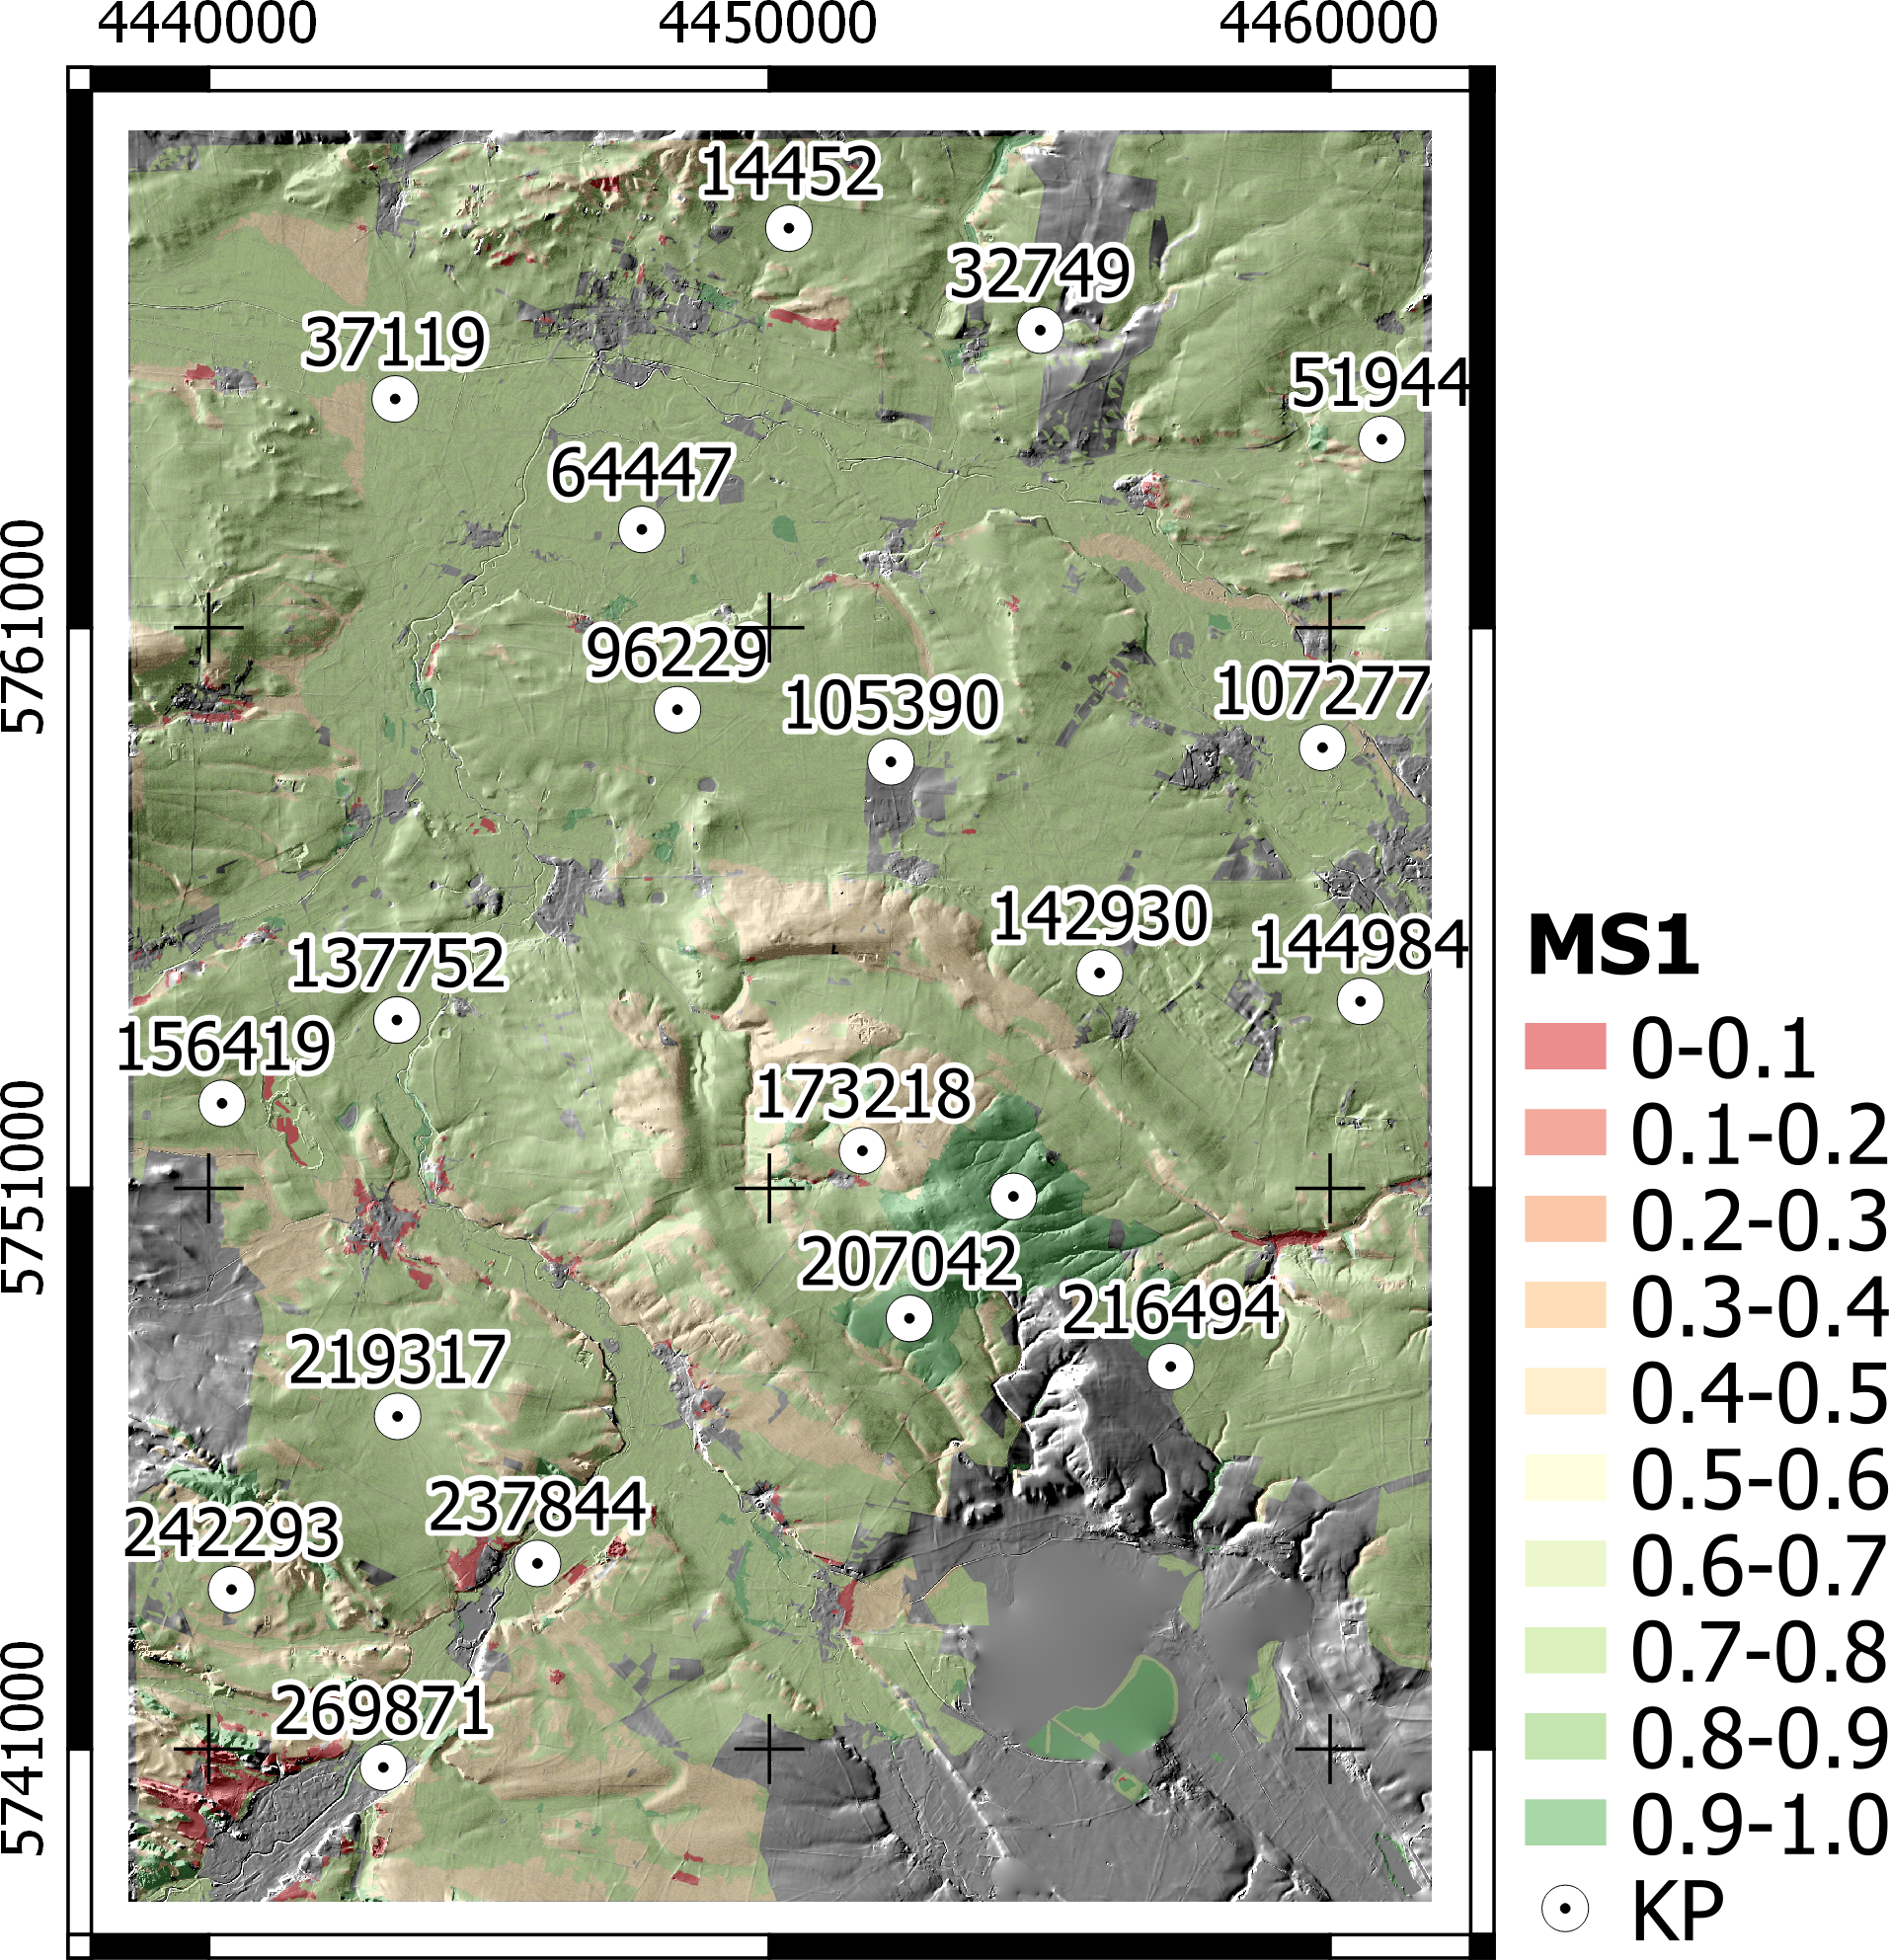
\includegraphics[height=0.48\textwidth]{figures/Genese_Schicht1MS1}}\quad
\subfigure[STB]{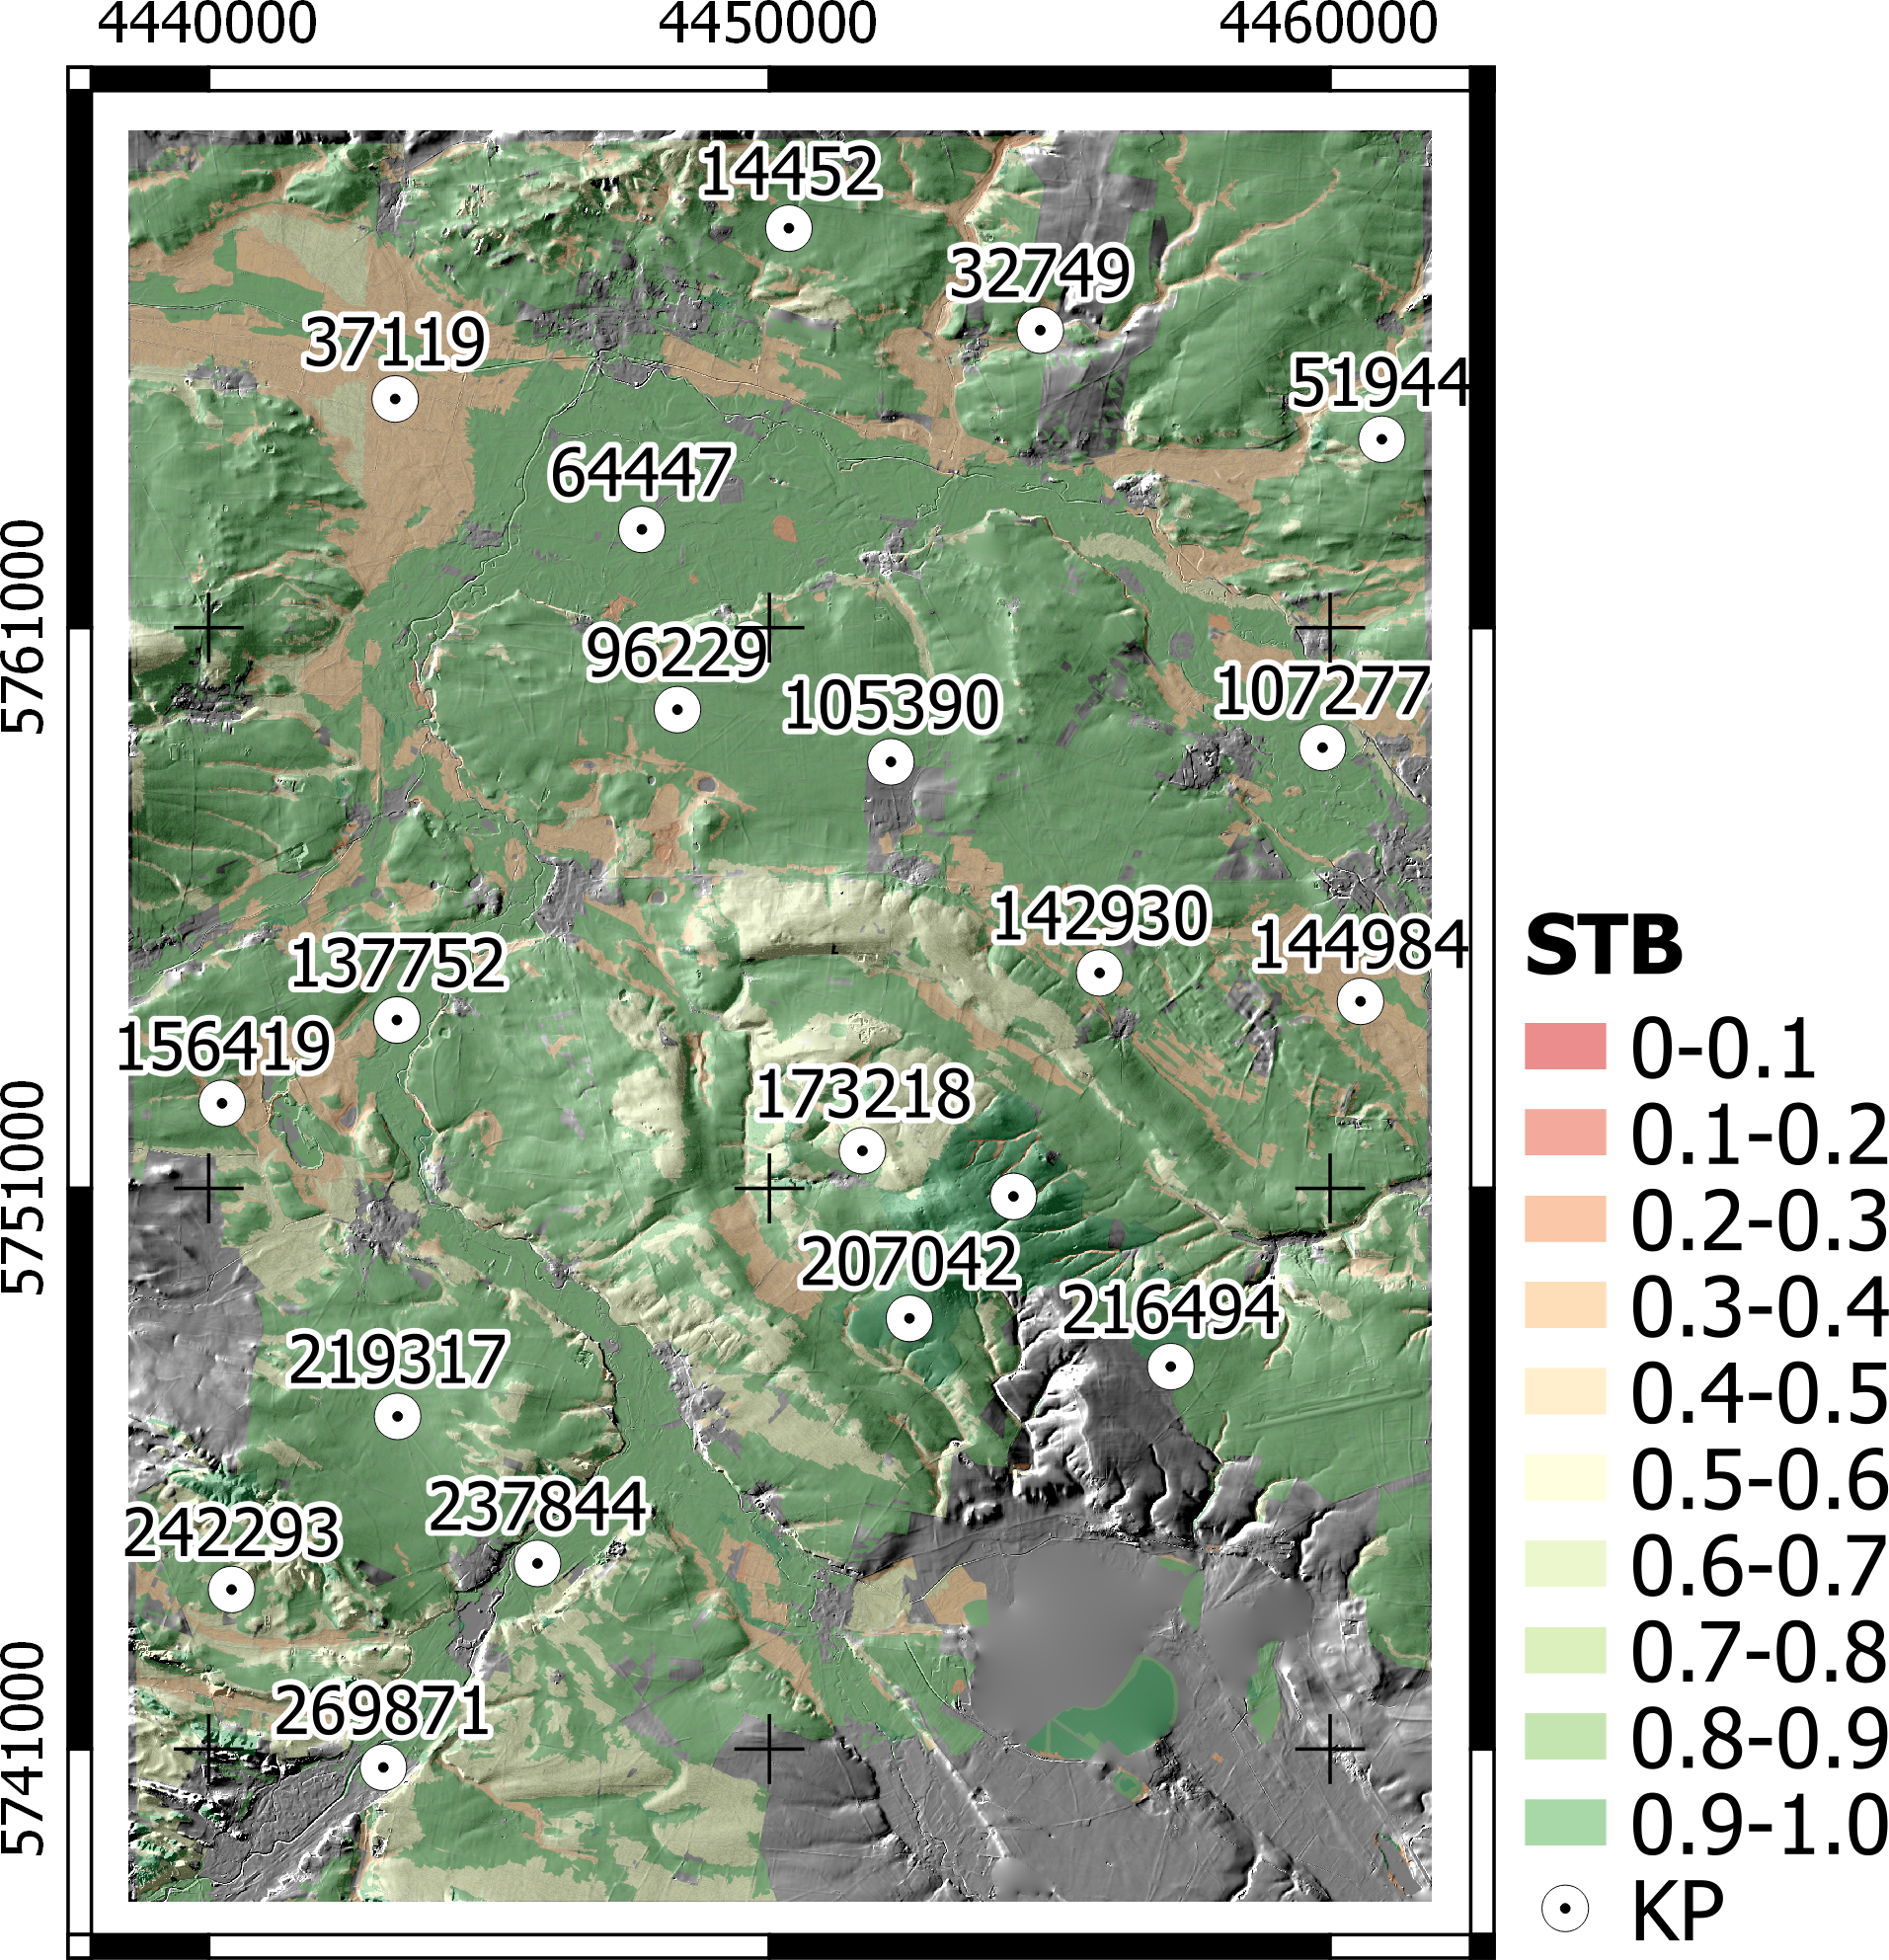
\includegraphics[height=0.48\textwidth]{figures/Genese_Schicht1STB}}
\caption{Qualitätsmaße \textit{MS1} und \textit{STB} für die Geneseklassifikation der Schicht 1 im Testgebiet \textit{Bode}.}\label{fig:GENESE-schicht1-qm}
\end{figure}

% Table generated by Excel2LaTeX from sheet 'Tabelle1'
\begin{sidewaystable}[p]
  \centering
  \caption[Ergebnis der Bodentypen-, Bodenartenhauptgruppen- und Bodenartengruppentypisiering für alle Schichten der Kontrollpunkte.]{Ergebnis der Bodentypen-, Bodenartenhauptgruppen- (BAHG\_) und Bodenartengruppentypisiering (BAG\_) für alle Schichten der Kontrollpunkte (vgl. Abb. \ref{fig:class_final}, \ref{fig:BAG-schicht1-qm} u. \ref{fig:GENESE-schicht1-qm}). MS1, STB -- Qualitätsmaße $|$ SRC -- Quelle $|$ v -- Vorläufige Bodenkarte 1:50\,000 $|$ g -- Geologische Karte 1:25\,000 $|$ f -- Forstliche Standortskartierung $|$  b -- Bodenschätzung, $|$ m -- Mittelmaßstäbige Landwirtschaftliche Standortskartierung.}\label{tab:KP-CLASS1}
        \begin{tabular8}{r|l|l|l|l|l|l}\toprule
    \textbf{ID} & \textbf{Bodentyp} & \textbf{BAHG}  & \textbf{BAG}   & \textbf{BAG\_STB} & \textbf{BAG\_MS1} & \textbf{BAG\_SRC} \\\midrule
    14452 & TT-LL & u(13)l & lu(13)tl & 1(4)0.8(11)0.2(13)0.8 & 1(13)0.8 & bs,f(13)gk \\\midrule
    32749 & TC    & t(4)u(6)t(11)u & ut(4)tu(6)ut(11)lu & 0.5(11)0.8 & 1(11)0.8 & bs,f(11)gk \\\midrule
    37119 & GGh   & l(11)s & ll(4)tl(11)ls & 0.5(4)0.8(7)0.3(11)0.3(13)0.8 & 1(7)0.5(11)0.8 & bs,f(7)v(11)gk \\\midrule
    51944 & DD-TT & u(6)l(8)u(11)l & lu(6)ll(8)lu(11)tl & 1(4)0.8(6)0.5(8)0.8(11)0.3(13)0.8 & 1(11)0.8 & bs,f(11)gk \\\midrule
    64447 & AT    & l(4)u(11)ste & tl(4)tu(11)ste & 0.8(4)0.5(11)0.3(13)0.8 & 1(11)0.8 & bs,f(11)gk \\\midrule
    96229 & DD-TT & u(11)s & lu(11)ls & 1(4)0.8(11)0.3(13)0.8 & 1(11)0.8 & bs,f(11)gk \\\midrule
    105390 & DD-TT & u(11)s & lu(11)ls & 1(4)0.8(11)0.3(13)0.8 & 1(11)0.8 & bs,f(11)gk \\\midrule
    107277 & AB    & l(3)t(13)??(20)s & tl(3)ut(13)??(20)ls & 0.5(3)0.8(11)0.6 & 1(11)0.8(13)0(20)0.8 & bs,f(11)gk \\\midrule
    137752 & gAT   & l(4)t(7)l(11)ste & tl(4)ut(7)tl(11)ste & 0.8(4)0.5(7)0.8(9)0.3(11)0.3(13)0.8 & 1(9)0.5(11)0.8 & bs,f(9)v(11)gk \\\midrule
    142930 & BB-TT & u(11)s & lu(11)ls & 1(4)0.8(11)0.3(13)0.8 & 1(11)0.8 & bs,f(11)gk \\\midrule
    144984 & DD-TC & u(13)??(20)l & tu(6)lu(13)??(20)tl & 0.5   & 1(13)0(20)0.8 & bs,f \\\midrule
    156419 & rGGc-GGh & l(3)u(9)l(11)hne & tl(3)tu(9)tl(11)hne & 0.8(3)0.5(9)0.3(11)0.3(13)0.8 & 1(9)0.5(11)0.8 & bs,f(9)v(11)gk \\\midrule
    173218 & RZ-DD & u(6)l(11)ste & lu(6)tl(11)ste & 0.8(6)0.3(11)0.3(13)0.8 & 1(6)0.5(11)0.8 & bs,f(6)v(11)gk \\\midrule
    184868 & BB-RZ & u(11)ste & lu(11)ste & 1(3)0.5(11)0.3(13)0.8 & 1(3)0.5(11)0.8 & bs,f(3)v(11)gk \\\midrule
    207042 & LF    & u(11)l & lu(11)tl & 0.8(6)0.3(11)0.3(13)0.8 & 1(6)0.5(11)0.8 & bs,f(6)v(11)gk \\\midrule
    216494 & LF    & u     & lu    & 1(6)0.5(13)0.8 & 1(13)0.8 & bs,f(13)gk \\\midrule
    219317 & RZ    & u(11)l & lu(11)tl & 1(4)0.8(11)0.3(13)0.8 & 1(11)0.8 & bs,f(11)gk \\\midrule
    237844 & AB    & l(3)u(5)t(11)ste & tl(3)lu(5)ut(11)ste & 0.8(3)0.5(11)0.3(13)0.8 & 1(11)0.8 & bs,f(11)gk \\\midrule
    242293 & DD    & u(3)l(4)u(6)s & tu(3)tl(4)lu(6)ls & 0.5(4)0.3(7)0.5(11)0.8 & 1(4)0.5(11)0.8 & bs,f(4)v(11)gk \\\midrule
    269871 & AT    & u(6)t(13)??(20)s & tu(6)ut(13)??(20)ls & 0.5(11)0.3 & 1(11)0.8(13)0(20)0.8 & bs,f(11)gk \\\bottomrule
    \end{tabular8}%
\end{sidewaystable}%

\begin{sidewaystable}[p]
  \centering
  \caption[Ergebnis der Bodentypen- und Genesetypisierung für alle Schichten der Kontrollpunkte.]{Ergebnis der Bodentypen- und Genesetypisierung (GEN\_) für alle Schichten der Kontrollpunkte (vgl. Abb. \ref{fig:class_final}, \ref{fig:BAG-schicht1-qm} u. \ref{fig:GENESE-schicht1-qm}). MS1, STB -- Qualitätsmaße $|$ SRC -- Quelle $|$ v -- Vorläufige Bodenkarte 1:50\,000 $|$ g -- Geologische Karte 1:25\,000 $|$ f -- Forstliche Standortskartierung $|$  b -- Bodenschätzung, $|$ m -- Mittelmaßstäbige Landwirtschaftliche Standortskartierung.}\label{tab:KP-CLASS2}
            \begin{tabular8}{r|l|l|l|l|l}\toprule
    \textbf{ID} & \textbf{BOD\_TYP} & \textbf{GEN}   & \textbf{GEN\_STB} & \textbf{GEN\_MS1} & \textbf{GEN\_SRC} \\\midrule
    14452 & TT-LL & p(11)pfl(20)g & 0.8(11)0.3(13)0.8 & 0.8   & gk \\\midrule
    32749 & TC    & uz(13)??(20)uz & 0.3   & 0.8(13)0(20)0.8 & gk \\\midrule
    37119 & GGh   & fl(6)f & 0.3(13)0.8 & 0.8   & gk \\\midrule
    51944 & DD-TT & p(11)pfl(20)g & 0.8(11)0.3(13)0.8 & 0.8   & gk \\\midrule
    64447 & AT    & fo(11)ff(20)fp & 0.8(11)0.3(13)0.8 & 0.8   & gk \\\midrule
    96229 & DD-TT & p(20)fg & 0.8   & 0.8   & gk \\\midrule
    105390 & DD-TT & p(20)fg & 0.8   & 0.8   & gk \\\midrule
    107277 & AB    & fo(13)??(20)ff & 0.8   & 0.8(13)0(20)0.8 & gk \\\midrule
    137752 & gAT   & fo(11)ff(20)fp & 0.8(11)0.3(13)0.8 & 0.8   & gk \\\midrule
    142930 & BB-TT & p(20)fg & 0.3(13)0.8 & 0.8   & gk \\\midrule
    144984 & DD-TC & fp(13)??(20)g & 0.3   & 0.8(13)0(20)0.8 & gk \\\midrule
    156419 & rGGc-GGh & og(13)??(20)og & 0.3   & 0.8(13)0(20)0.8 & gk \\\midrule
    173218 & RZ-DD & p(20)n & 0.5(11)0.8 & 0.5(11)0.8 & v(11)gk \\\midrule
    184868 & BB-RZ & p(20)n & 1(13)0.8 & 1(13)0.8 & bs,f(13)gk \\\midrule
    207042 & LF    & p(13)pfl(20)g & 1(11)0.2(13)0.8 & 1(13)0.8 & bs,f(13)gk \\\midrule
    216494 & LF    & p(13)??(20)p & \multicolumn{1}{r}{1} & 1(13)0(20)0.8 & bs,f \\\midrule
    219317 & RZ    & p(11)pfl(20)g & 0.8(11)0.3(13)0.8 & 0.8   & gk \\\midrule
    237844 & AB    & fo(11)ff & 0.8(11)0.3(13)0.8 & 0.8   & gk \\\midrule
    242293 & DD    & p(20)s & 0.8   & 0.8   & gk \\\midrule
    269871 & AT    & fo(13)??(20)ff & 0.8   & 0.8(13)0(20)0.8 & gk \\\midrule
    \end{tabular8}%
\end{sidewaystable}%

In Abbildung \ref{fig:class_final} sind die Ergebnisse der Bodenartengruppen- und Geneseklassifikation für die erste Schicht und das gesamte Untersuchungsgebiet dargestellt. Danach dominieren die Bodenartengruppen \textit{lu}, \textit{tu} und \textit{tl} sowie die Geneseklassen \textit{p} und \textit{fo}. Die Abbildungen \ref{fig:BAG-schicht1-qm} und \ref{fig:GENESE-schicht1-qm} zeigen die korrespondieren Qualitätsmaße. Für die überwiegenden Fläche des Testgebietes \textit{Bode} stehen demzufolge für die Schicht 1 Bodeneingangsdaten hoher Qualität zur Verfügung, was durch hohe \textit{MS1}-Werte ausgedrückt wird. Mithilfe des Qualitätsmaßes \textit{STB} lassen sich Flächen identifizieren, die durch widersprüchliche Ergebnisse gekennzeichnet sind. Das betrifft im Untersuchungsgebiet beispielsweise weite Teile der Auenbereiche, wo oft die Angaben der Bodenschätzung und VBK\,50 zu unterschiedlichen Bodenartengruppen-Klas"-si"-fi"-zie"-rung  führen (vgl. Tab. \ref{tab:KP-CLASS1}: Kontrollpunkte 32749, 37119, 107277 u. 269871). Geringe Stabilitäten bei der Ge"-nese-Klas"-si"-fi"-zie"-rung sind in der Regel auf Widersprüche zwischen der VBK\,50 und der GK\,25 zurückzuführen (vgl. Tab. \ref{tab:KP-CLASS2}: Kontrollpunkte 32749 u. 37119).

\subsection{Typisierung}\label{sec:typ}
Die Typisierung zielt auf die vertikale Zusammenfassung der schichtspezifischen Klas"-si"-fi"-zie"-rungsergebnisse und Qualitätsmaße der Bodenparameter. In den Tabellen \ref{tab:KP-CLASS1} und \ref{tab:KP-CLASS2} sind die Bodensubtypen sowie die aggregierten Schichtinformationen der klassifizierten Bodenartengruppen und -hauptgruppen sowie der Geneseklassen für die Kontrollpunkte aufgelistet. So repräsentiert der Kontrollpunkt 207042 den Bodentyp \textit{Fahlerde}.  Als Bodenartengruppen bzw. -hauptgruppen wurden \textit{lu} bzw. \textit{u} bis zu einer Tiefe von 10\,dm sowie ab 11\,dm \textit{tl} bzw. \textit{l} ausgewiesen. Die \textit{MS1}-Werte zeigen, dass das Profil auf der Grundlage der Informationsquellen FSK, VBK\,50 und GK\,25 zusammengesetzt worden ist. Die Stabilitätswerte (\textit{STB}) machen deutlich, dass die Klassifikationsergebnisse durch Widersprüche gekennzeichnet sind.  Das betrifft die ersten 12\,dm, wo die Klassifikation von FSK und MMK ($<6$\,dm), VBK\,50 und MMK (6 bis 10\,dm) sowie GK\,25 und MMK (11 bis 12\,dm) zu unterschiedlichen Ergebnissen führten (vgl. Tab. \ref{tab:trans-ba}). Ab 13\,dm fungiert der Datensatz der GK\,25 als alleinige Informationsquelle.\

FSK und GK\,25  bilden die Informationsquelle zur Ableitung bodengenetischer Informationen. Als Ergebnis wurde bis 12\,dm  die Klasse \textit{p} und ab 13\,dm die Klasse \textit{pfl} ausgewiesen. Schicht 20 ist durch die Geneseklasse \textit{g} gekennzeichnet. Bei  11 und 12\,dm widersprechen sich beide Informationsquellen, was sich in einem \textit{STB}-Wert von 0,2 niederschlägt (vgl. Tab. \ref{tab:trans-gen}, S. \pageref{tab:trans-gen}).\

Die Beispiele zeigen, dass die Klassifikations- und Typisierungsergebnisse jeder Bezugseinheit hinsichtlich ihrer Qualität dokumentiert sind. Darüber hinaus können  für jede Bezugseinheit und Schicht die für die Klassifikation bestimmenden Bodeneingangsdaten identifiziert werden. 



\subsection{Reliefbezogene Plausibilitätsanalyse der Klassifikationsergebnisse}\label{sec:ext}
Die in den Kapiteln \ref{sec:transformation} bis \ref{sec:typ} beschriebenen Glieder der ProBoSA-Prozesskette können als Basisfunktionen angesehen werden. Das ProBoSA-System erlaubt es, zusätzliche Analysefunktionen zu integrieren, was am Beispiel eines Reliefklassifikationsmoduls veranschaulicht wird. Die Funktion ist ebenfalls innerhalb der Programmumgebung \textbf{R} umgesetzt worden und gliedert sich in die Schritte

\begin{compactenum}
	\item Parametrisierung der Bezugseinheiten mit Reliefattributen (Kap. \ref{sec:ext-ta})
	\item Auendetektion (Kap. \ref{sec:ext-fp}) und
	\item Reliefgliederung terrestrischer Bezugseinheiten (Kap. \ref{sec:ext-sf}).
\end{compactenum}


In Kapitel \ref{sec:ext-ps} wird schließlich gezeigt, wie die Ergebnisse der Reliefgliederung für einfache Plausibilitätsanalysen genutzt werden können.

\subsubsection{Parametrisierung der Bezugseinheiten mit Reliefattributen}\label{sec:ext-ta}


Die Zuweisung der Reliefattribute zu den Bezugseinheiten (Kap. \ref{sec:be}) ist mit dem \texttt{RSAGA}-Modul realisiert worden \citep{Brenning2008rsaga}, das die Nutzung von Reliefanalyse-Funktionalitäten von SAGA GIS innerhalb von \textbf{R} ermöglicht \citep{Conrad-etal2015gmd}. Der Programmcode \ref{prog:ta} dokumentiert die programmtechnische Umsetzung. Danach werden zunächst alle Reliefattribute, die hier im \texttt{*.asc}-Format vorliegen, in die Liste \texttt{l.r} überführt. Anschließend werden alle Listenelemente innerhalb einer Schleifen-Umgebung in das SAGA-Format \texttt{*.sgrd} mittels der Funktion \texttt{rsaga.esri.to.sgrd()} importiert. Die \texttt{rsaga.geoprocessor()}-Umgebung ermöglicht den formalisierten Zugriff auf SAGA GIS-Module. Hier wird das Modul 2 der \texttt{shapes\_grid}-Bib"-lio"-thek verwendet. Dahinter verbirgt sich eine \textit{zonal statistics}-Funktion, mit der für jedes Polygon des Vektordatensatzes der Mittelwert basierend auf den Werten des Rasterdatensatzes berechnet wird.


\begin{program}[t] 
\begin{verbatim}
l.r <- list.files(pattern="*.*\\.asc$") 
for (i in 1:length(l.r)){
  #Import
  rsaga.esri.to.sgrd(
    in.grids=l.r[i], 
    out.sgrds=paste(substr(l.r[i],0,nchar(l.r[i])-4),c(".sgrd"),sep=""), 
    in.path=getwd(),env=myenv)
  ##zonal statistics
  rsaga.geoprocessor(
    lib="shapes_grid",
    module=2,
    param=list(GRIDS=paste(substr(l.r[i],0,nchar(l.r[i])-4),c(".sgrd"),sep=""),
               POLYGONS=file.path(w.dir,result.dir,result.shp),
               COUNT=0,
               MIN=0,
               MAX=0,
               RANGE=0,
               SUM=0,
               VAR=0,
               STDDEV=0,
               QUANTILE=0,
               NAMING=1),
    env=myenv)
  setTxtProgressBar(pb, i)
}
\end{verbatim}
\caption{\textbf{R}-Programmcode zum Import von Reliefattributen und zur Parametrisierung von Bezugseinheiten.} 
\label{prog:ta} 
\end{program} 

Für die Reliefgliederung sind die kombinierten Reliefattribute \textit{Massenbilanzindex} ($MBI$) sowie zwei Varianten des \textit{Reliefklassifikationsindex} ($RKI1$ und $RKI2$) mit den Bezugseinheiten in Beziehung gesetzt worden:

\begin{itemize}
	\item Das Attribut $MBI$ kombiniert die Basisattribute \textit{Wölbung}, \textit{Neigung} und \textit{Höhe über Tiefenlinie} und erlaubt die Detektion von konkaven und konvexen Reliefformen \citep{Moeller-etal2008jpnss,Moeller-etal2012catena,MoellerVolk2015geoderma}.
	\item Die Kombination der Reliefattribute \textit{Bodenfeuchteindex} und \textit{Höhe über Tiefenlinie} bzw. \textit{Höhe über Fließgewässer}   ergibt die Reliefklassifikationsindizes \textit{RKI2} bzw. \textit{RKI1} \citep{Bock-etal2007}, die für die vertikale Reliefgliederung von Landschaften entwickelt worden sind.
\end{itemize}

\begin{figure}[t]
\centering\subfigure[Räumliche Cluster-Verteilung]{\includegraphics[height=0.62\textwidth]{figures/BT1_MC-FP_RKI2__MEAN__map.png}}\quad
\centering\subfigure[Cluster-Boxplots und $RKI2$-Werteverteilung]{\includegraphics[height=0.62\textwidth]{figures/BT-BA-GEN_epsg31468_RKI2_floodplain.pdf}}
\caption{Ergebnisse der Clusteranalyse des Reliefattributes $RKI2$ zur Auendetektion im Testgebiet \textit{Bode}.}\label{fig:class-floodplain}
\end{figure}

\subsubsection{Auendetektion}\label{sec:ext-fp}
Im Programmcode \ref{prog:tc} zur Auendetektion wird eine vom Nutzer festzulegende Variable \texttt{ta.fp} einer Clusteranalyse mit dem Algorithmus \texttt{mclust} unterzogen \citep{FraleyRaftery2002jasa}. Auen können als Prozessbereiche angesehen werden, die die Kriterien \textit{minimale Höhe über Fließgewässer}, \textit{minimale Neigung} und  \textit{maximale Fließakkumulation}  erfüllen und durch das  Reliefattribut $RKI2$ repräsentiert werden. Mit der Cluster-Analyse werden statistisch signifikante Grenzen in der $RKI2$-Werteverteilung bestimmt (Abb. \ref{fig:class-floodplain}b), die in Abbildung  \ref{fig:class-floodplain}a räumlich abgebildet werden. Im Testgebiet werden die Cluster 1 und 2 als Auenbereiche betrachtet.

\begin{program}[t]
\begin{verbatim}
#Floodplain detection 
MC <- Mclust(model.matrix(~-1 + s@data[[c(ta.fp)]],s@data))
s@data$MC.FP <- MC$classification
#Selection of floodplain cluster
s@data$FP <- ifelse(s@data$MC.FP<3,1,0)
#Clustering of terrestrial process domains
s@data$MC1 <- ifelse(s@data$FP==0,
              Mclust(model.matrix(~-1 + s@data[[c(ta1.sf)]],
							s@data),G=CN)$classification,
                    0)
s@data$MC2 <- ifelse(s@data$FP==0,
              Mclust(model.matrix(~-1 + s@data[[c(ta2.sf)]],
							s@data),G=CN)$classification,
                     0)
#combining MC1 and MC2
s@data$TC <- interaction(as.factor(s@data$MC1), as.factor(s@data$MC2), sep="")
\end{verbatim}
\caption{\textbf{R}-Programmcode zur Clusteranalyse, Auendetektion und Reliefgliederung terrestrischer Bezugseinheiten.} 
\label{prog:tc} 
\end{program} 

\begin{figure}[p]
\centering\subfigure[Räumliche Cluster-Verteilung des Reliefattributes $MBI$]{\includegraphics[height=0.62\textwidth]{figures/BT1_MC1_MBI__MEAN__map.png}}\quad
\centering\subfigure[Räumliche Cluster-Verteilung des Reliefattributes $RKI1$]{\includegraphics[height=0.62\textwidth]{figures/BT1_MC2_RKI1__MEAN__map.png}}\quad

\centering\subfigure[Cluster-Boxplots und $MBI$- bzw. $RKI1$-Werteverteilung]{\includegraphics[height=0.6\textwidth]{figures/bezugseinheiten_1_MBI-RKI1_TC-boxplots.pdf}}
\caption{Ergebnisse der Clusteranalyse des Reliefattribute $MBI$ und $RKI1$ zur Gliederung der terrestrischen Prozessbereiche im Testgebiet \textit{Bode}.}\label{fig:class-terr}
\end{figure}

\subsubsection{Reliefgliederung terrestrischer Bezugseinheiten}\label{sec:ext-sf}
Bei der Reliefgliederung der terrestrischen Bezugseinheiten werden die Reliefattribute $MBI$ (\texttt{ta1.sf}) und $RKI1$ (\texttt{ta2.sf}) getrennt geclustert, wobei die Clusteranzahl \texttt{CN} vom Nutzer zu bestimmen ist (Programmcode \ref{prog:tc}). Die Ergebnis-Cluster werden mit Hilfe der Funktion \texttt{interaction} zusammengeführt.\ 

Abbildung \ref{fig:class-terr} zeigt die Ergebnisse der Clusteranalyse. Danach repräsentiert die Cluster-Nummer 0 die detektierten Auenbereiche. Über die kombinierte Auswertung der $MBI$- und $RKI1$-Cluster können Reliefformen beschrieben werden. So lassen sich die Kombination der Cluster $C_{MBI}=5$ und $C_{RKI1}=5$ als stark konvexe Scheitelbereiche oder die Kombination der Cluster $C_{MBI}=1$ und $C_{RKI1}=1$ als Senkenbereiche am Rande von Auenbereichen interpretieren.

\begin{figure}[p]
\centering
\subfigure[]{\includegraphics[width=0.75\textwidth]{figures/BT1_MBI-RKI1_TC.pdf}}

\centering\subfigure[]{\includegraphics[width=0.48\textwidth]{figures/bezugseinheiten_1_BAG_TC.pdf}}
\centering\subfigure[]{\includegraphics[width=0.48\textwidth]{figures/bezugseinheiten_1_GEN_TC.pdf}}

\caption[Anteile von Bodenklassen, Bodenartengruppen und Geneseklassen an der Reliefklasse \textit{Aue}.]{Anteile von Bodenklassen (a), Bodenartengruppen (b) und Geneseklassen (c) an der Reliefklasse \textit{Aue}.}\label{fig:soptep-fp}
\end{figure}

\subsubsection{Plausibilitätsanalyse}\label{sec:ext-ps}
Ähnlich der Herangehensweise in \citet{Moeller-etal2012catena} ermöglichen Reliefklassen, Klassifikationsergebnisse einer reliefspezifischen Plausibilitätsanalyse zu unterziehen. Das heißt, dass durch den Nutzer die Kombination von spezifischen Relief- und Bodenklassen abgefragt werden kann. Abbildung \ref{fig:soptep-fp} zeigt ein Abfragebeispiel für die Anteile von Bodenklassen (a), Bodenartengruppen (b) und Geneseklassen (c) in der Reliefklasse \textit{Aue}. Als plausibel können beispielweise die Kombinationen mit der Bodenklasse \textit{Auenboden}, den Geneseklassen \textit{fo} und \textit{fp} oder den Bodenartengruppen \textit{tl} und \textit{tu} angesehen werden. Nicht plausibel ist dagegen die Kombination mir der Bodenklasse \textit{Schwarzerden}, der Geneseklasse \textit{p} oder der Bodenartengruppe \textit{lu}.




\section{Zusammenfassung}\label{sec:fazit}
Ziel des Projektes ProBoSA war die (semi)automatischen Homogenisierung von bodenkundlichen Datengrundlagen entsprechend den Vorgaben der aktuellen bodenkundlichen Kartieranleitung \citep{KA5}. Dabei wurden Informationen zusammengeführt, die sich hinsichtlich ihrer Nomenklaturen, thematischen Komplexität und  Aufnahmemethoden unterscheiden. Eine besondere Herausforderung bestand dabei in der Erarbeitung von reproduzierbaren Datenintegrationsregeln sowie in der Formalisierung von Expertenwissen. Die Datenintegrationsprozedur ist für die Substratmerkmale Feinboden, Genese sowie Carbonat- und Skelettgehalt angewendet worden. Die Transformation der bodentypologischen Informationen erfolgte durch eine direkte Interpretation der Bodenschätzung, der  Forstlichen Standortskartierung und der Geologischen Karte 1:25\,000.\ 

Der wichtigste Schritt der Datenintegration bestand in der Entwicklung von Transformationstabellen, in denen die Regeln zur inhaltlichen Übersetzung  der Ausgangsdatensätze in die KA\,5-Nomenklatur formalisiert worden sind. Voraussetzung war die schichtweise Zerlegung der Ausgangsdatensätze. Dazu wurden an die Nomenklatur der Ausgangsdatensätze angepasste automatische Prozeduren zur Trennung von Zeichenketten entwickelt.\ 

Bei der Klassikation wurden die Transformationsergebnisse schichtweise zusammengefasst, wobei in Abhängigkeit vom Ausgangsdatensatz Wichtungen berücksichtigt worden sind. Die anschließende Typisierung aggregierte die schichtspezifischen Klassifikationsergebnisse zu Zeichenketten. Als Ergebnis konnten für jedes Zielmerkmal, jede Schicht und jede Bezugseinheit Qualitätsmaße abgeleitet werden.\

Die Datenintegrationsschritte wurden in ein ProBoSA-System als ausführbare Programme zusammengefasst. Innerhalb des ProBoSA-Systems existieren Schnittstellen, um Expertenwissen reproduzierbar vorzuhalten. Das betrifft vor allem die Erstellung von Transformationstabellen und die Datenwichtung bei der Klassififikation der Zielmerkmale. Weiterhin kann die ProBoSA-Prozedur auf beliebige Bezugseinheiten angewendet werden. Schließlich erlaubt die offene Struktur des ProBoSA-Systems die Integration weiterer Komponenten. So ist innerhalb des Projektes das Datenintegrationsergebnis um Reliefparameter und -klassen erweitert worden.
\newpage




\section{Ausblick}
Die im Pilotprojekt entwickelte Vorgehensweise kann als Blaupause für eine landesweite Integration von bodenkundlich relevanten Datengrundlagen angesehen werden. Dazu gehört auch die Kopplung räumlicher Bezugseinheiten (z.B. Rasterzellen, Konturen) mit beliebigen Flächendatensätzen (z.B. Reliefeigenschaften oder Satellitenbildindizes).\

Das mit dem ProBoSA-System generierte Datenintegrationsergebnis ermöglicht für spezifische Bodenklassen und -parameter 

\begin{compactitem}
	\item eine vertikale Kombination verschiedener Datenquellen und 
	\item die Identifikation von Widersprüchen verschiedener Datenquellen.
\end{compactitem}

Damit ist die Voraussetzung geschaffen worden, um typisierte Substratabfolgen nach bodenkundlichen und/oder geologischen Standards abzuleiten. Weitere Arbeiten sollten    die Entwicklung von Regeln zur  Prüfung logischer Schichtabfolgen beinhalten. Das betrifft vor allem die Kombinationsergebnisse aus Bodenschätzung und GK\,25.\ 

Ebenfalls notwendig erscheinen Arbeiten an einer weiteren Verbesserung der Transformation der Grablochbeschriebe. Dazu gehören beispielsweise Informationen zur Steinigkeit und anstehender Festgesteinsschichten und deren Verwitterungsdecken. Der bisher erreichte Stand ist noch nicht ausreichend, um die mit Hilfe des NIBIS-Schlüssels \citep{NBIS2003} erarbeiteten thematischen Auswertungskarten  überarbeiten zu können \citep{Hartmann2006}.\

Der für das Testgebiet erarbeitete bodentypologische Transformationsschlüssel ist außerhalb des ProBoSA-System entwickelt und getestet worden. Eine Integration in das ProBoSA-System wäre noch anzustreben. In diesem Zusammenhang sollten weitere bodenkundlich relevante Datenquellen wie Informationen zum Grundwasserflurabstand oder Klima einbezogen werden.\

Die Anwendung von geostatistischen Methoden oder Verfahren des maschinellen Lernens zur Prognose von Bodenklassen oder -parametern erfordert Trainingsdatensätze. In diesem Zusammenhang kann das mit dem ProBoSA-System generierte Datenintegrationsergebnis als Basisdatensatz betrachtet werden, um Trainingsdatensätze hoher Primärdatenqualität abzuleiten oder weitere inhaltliche Filteroperationen anzuwenden. Zu Letzteren gehören beispielsweise Verfahren der reliefbedingten Plausibilität, wie sie bereits im LAGB angewendet worden sind \citep[vgl. Kap. \ref{sec:dsm}; ][]{Moeller-etal2012catena,Hartmann2014}.


